\documentclass[14pt,a4paper]{extarticle}

\usepackage{subcaption}

% ---------- Кодировка и язык ----------
\usepackage[T2A]{fontenc}
\usepackage[utf8]{inputenc}
\usepackage[russian]{babel}

% ---------- Геометрия ----------
\usepackage[
    left=30mm,
    right=15mm,
    top=20mm,
    bottom=20mm
]{geometry}

% ---------- Математика ----------
\usepackage{amsmath,amssymb}

% ---------- Графики, таблицы и изображения ----------
\usepackage{graphicx}
\usepackage{float}
\usepackage{booktabs}
\usepackage{array}
\usepackage{siunitx}
\usepackage{pgfplots}
\pgfplotsset{compat=1.18}

% ---------- Дополнительно ----------
\usepackage{indentfirst}
\usepackage{caption}
\usepackage{hyperref}

\setlength{\parindent}{1.25cm}
\setlength{\parskip}{0pt}

\begin{document}


% =========================================================
% ТИТУЛЬНЫЙ ЛИСТ
% =========================================================

\begin{titlepage}
    \centering

    {\large Московский Физико-Технический Институт\par}

    \vspace{4cm}

    {\large Лабораторная работа №3.6.1\par}

    \vspace{0.5cm}

    \rule{\textwidth}{0.4pt}

    \vspace{0.3cm}

    {\LARGE \textbf{Спектральный анализ электрических сигналов}\par}

    \vspace{0.3cm}

    \rule{\textwidth}{0.4pt}

    \vfill

    \begin{flushright}
        \begin{minipage}{0.42\textwidth}
            Выполнил:\\
            Студент 2 курса ФАКТ\\
            Группа Б03-502\\
            Подмосковнов Лев
        \end{minipage}
    \end{flushright}

    \vfill

    Долгопрудный\\
    2026

\end{titlepage}

% =========================================================
% ЦЕЛЬ И ОБОРУДОВАНИЕ
% =========================================================

\section*{Цель работы}

Изучить спектры сигналов различной формы и влияние параметров сигнала
на вид соответствующих спектров; проверить справедливость соотношений
неопределённостей; познакомиться с работой спектральных фильтров
на примере RC-цепочки.

\section*{Используемые приборы и материалы}

В работе использовались:
\begin{itemize}
    \item генератор сигналов специальной формы АКИП-3409/4;
    \item цифровой осциллограф SIGLENT АКИП 4131/1;
    \item RC-цепочка;
    \item соединительные кабели.
\end{itemize}

% =========================================================
% ТЕОРЕТИЧЕСКОЕ ВВЕДЕНИЕ
% =========================================================

\section{Теоретическое введение}

\subsection{Ряд Фурье и спектральный анализ}

Периодическая функция может быть представлена в виде ряда Фурье:
\begin{equation}
f(t)=\frac{A_0}{2}
+\sum_{n=1}^{\infty}
\left[
A_n\cos(2\pi\nu_n t)
+
B_n\sin(2\pi\nu_n t)
\right].
\end{equation}

Здесь
\[
\nu_n=n\nu_0,\qquad
\nu_0=\frac{1}{T}.
\]

Коэффициенты разложения:
\begin{equation}
A_n=\frac{2}{T}\int_0^T
f(t)\cos(2\pi\nu_n t)\,dt,
\end{equation}

\begin{equation}
B_n=\frac{2}{T}\int_0^T
f(t)\sin(2\pi\nu_n t)\,dt.
\end{equation}

В представлении амплитуд и фаз:
\begin{equation}
f(t)=\frac{a_0}{2}
+\sum_{n=1}^{\infty}
a_n\cos(2\pi\nu_n t+\varphi_n),
\end{equation}

где
\begin{equation}
a_n=\sqrt{A_n^2+B_n^2}.
\end{equation}

Спектром функции называют совокупность частот гармоник и соответствующих
им амплитуд.

\subsection{Соотношения неопределённостей}

Между характерным временем изменения сигнала $\Delta t$ и характерным
масштабом его спектра $\Delta\nu$ выполняется соотношение
\begin{equation}
\Delta\nu\,\Delta t\sim1.
\end{equation}

Для периодического сигнала с периодом $T$ расстояние между соседними
гармониками равно
\begin{equation}
\delta\nu=\frac{1}{T}.
\end{equation}

Для импульса характерной длительности $\tau$ характерная ширина спектра
имеет порядок
\begin{equation}
\Delta\nu\sim\frac{1}{\tau}.
\end{equation}

\subsection{Быстрое преобразование Фурье}

В эксперименте спектр сигнала определяется с помощью быстрого
преобразования Фурье (БПФ). При цифровом спектральном анализе существенны
частота дискретизации и конечная длительность регистрируемого временного
интервала.

\newpage

% =========================================================
% А
% =========================================================

\section{Исследование спектра периодической последовательности
прямоугольных импульсов}

\subsection{Цель опыта}

Исследовать спектр периодической последовательности прямоугольных
импульсов и проверить соотношения неопределённостей.

\subsection{Параметры сигнала}

На данном этапе использовалась периодическая последовательность
прямоугольных импульсов.

% TODO: вписать фактические параметры эксперимента

\begin{table}[H]
\centering
\caption{Параметры прямоугольного сигнала}
\begin{tabular}{|c|c|}
\hline
Параметр & Значение \\
\hline
$\nu_{\text{повт}}$ & 1 кГц\\
\hline
$T$ & 1 мс\\
\hline
$\tau$ & 50 мкс\\
\hline
\end{tabular}
\end{table}

\subsection{Наблюдение спектра}

Было исследовано изменение спектра периодической последовательности
прямоугольных импульсов при изменении частоты повторения импульсов
$\nu_{\text{повт}}$ и длительности импульса $\tau$.

При первом исследовании длительность импульса оставалась постоянной:
\[
\tau = 50~\text{мкс},
\]
а частота повторения изменялась от $1$ до $4$ кГц.

\begin{figure}[H]
    \centering

    \begin{subfigure}{0.48\textwidth}
        \centering
        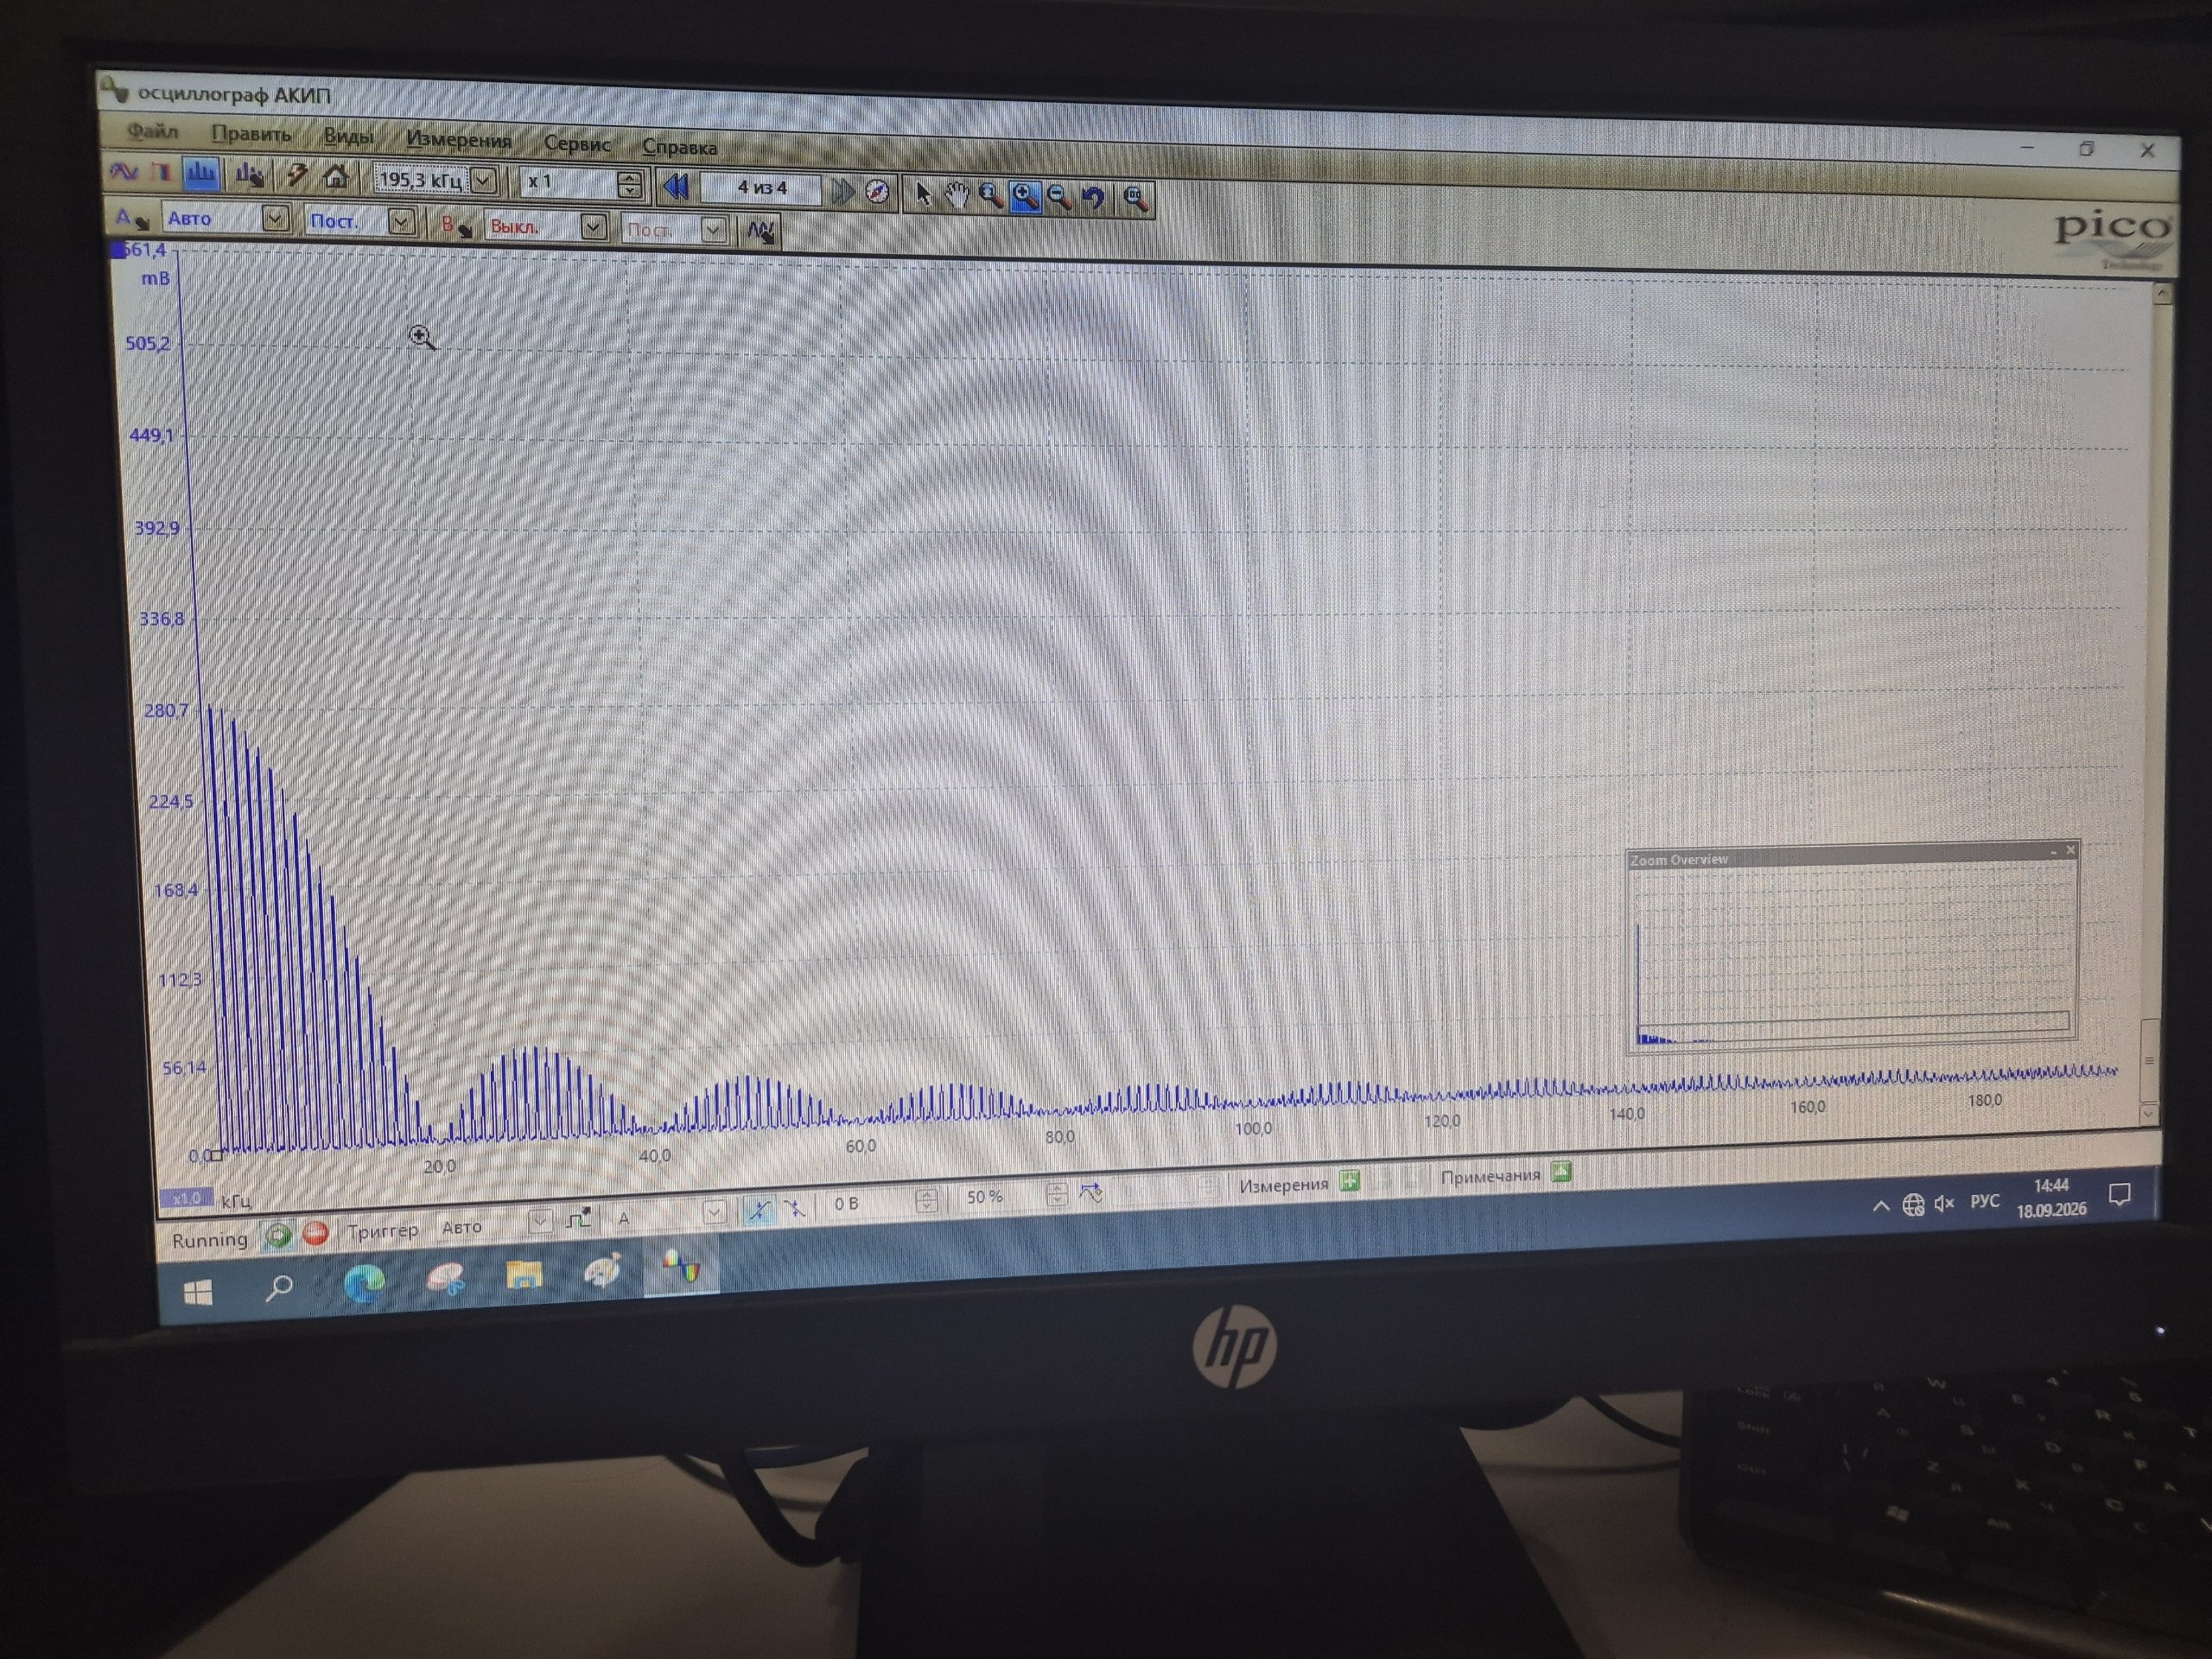
\includegraphics[width=\textwidth]{images/A_1kHz.jpg}
        \caption{$\nu_{\text{повт}}=1$ кГц}
    \end{subfigure}
    \hfill
    \begin{subfigure}{0.48\textwidth}
        \centering
        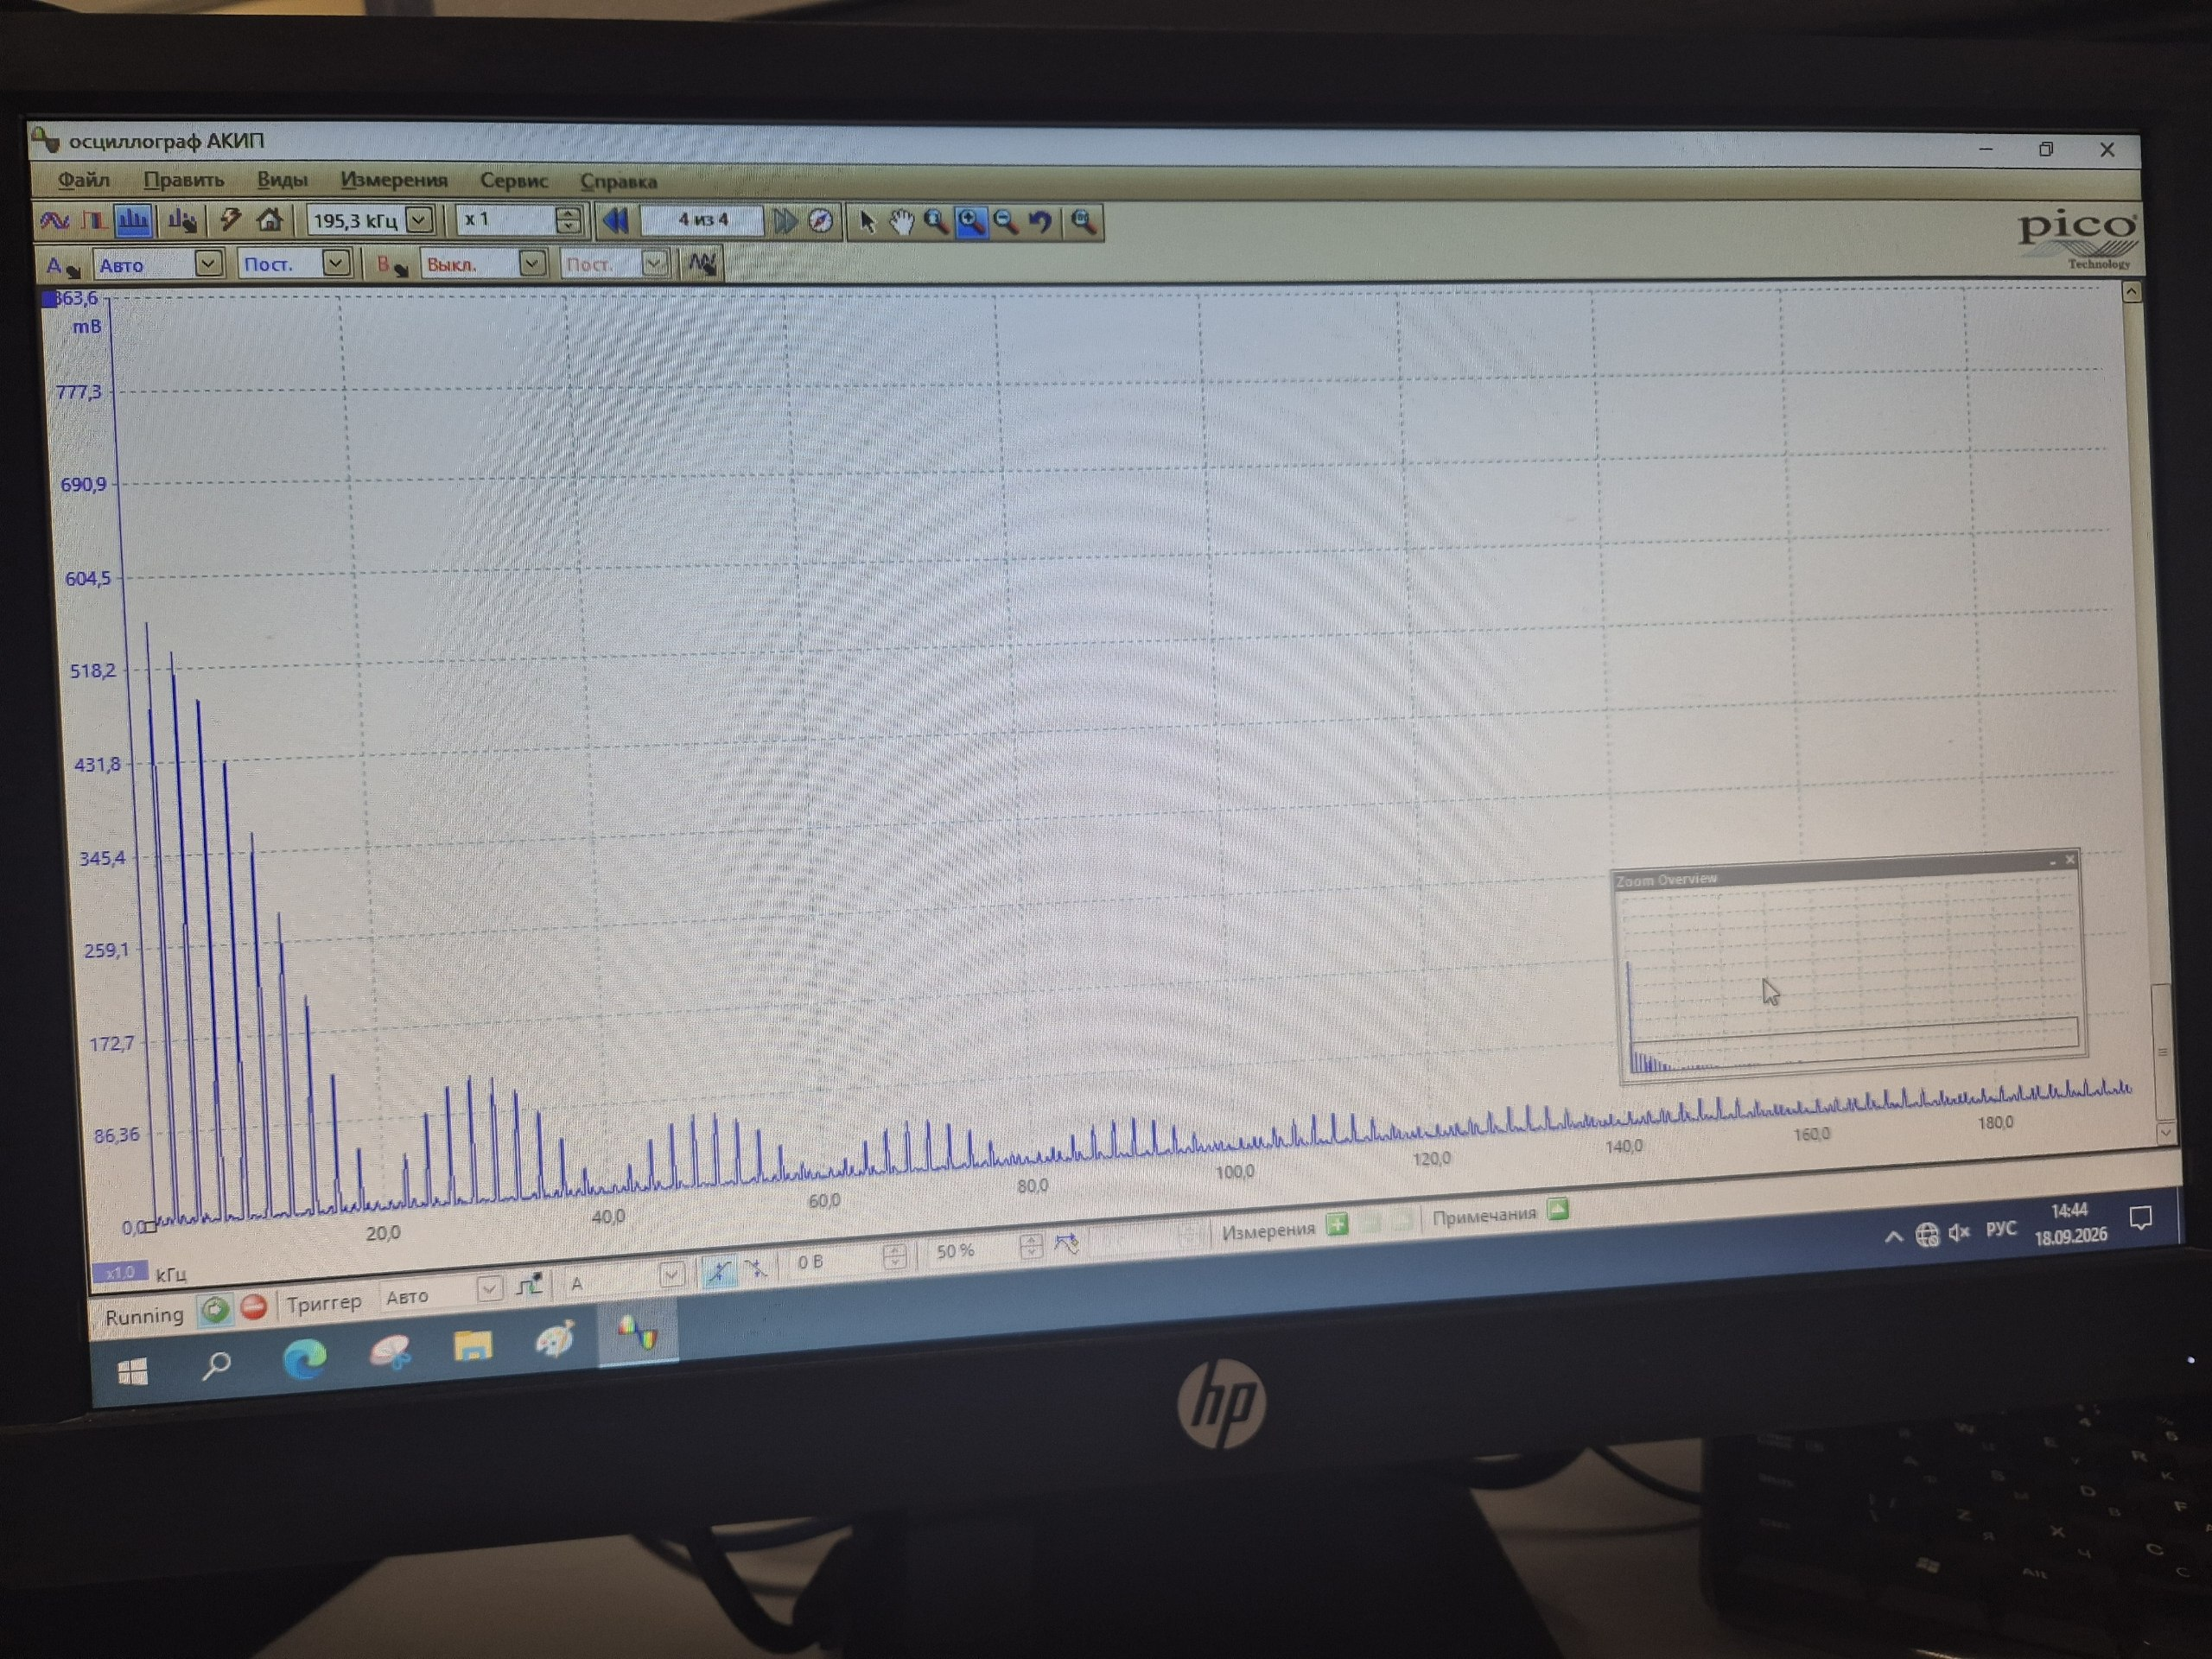
\includegraphics[width=\textwidth]{images/A_2kHz.jpg}
        \caption{$\nu_{\text{повт}}=2$ кГц}
    \end{subfigure}

    \vspace{0.5cm}

    \begin{subfigure}{0.48\textwidth}
        \centering
        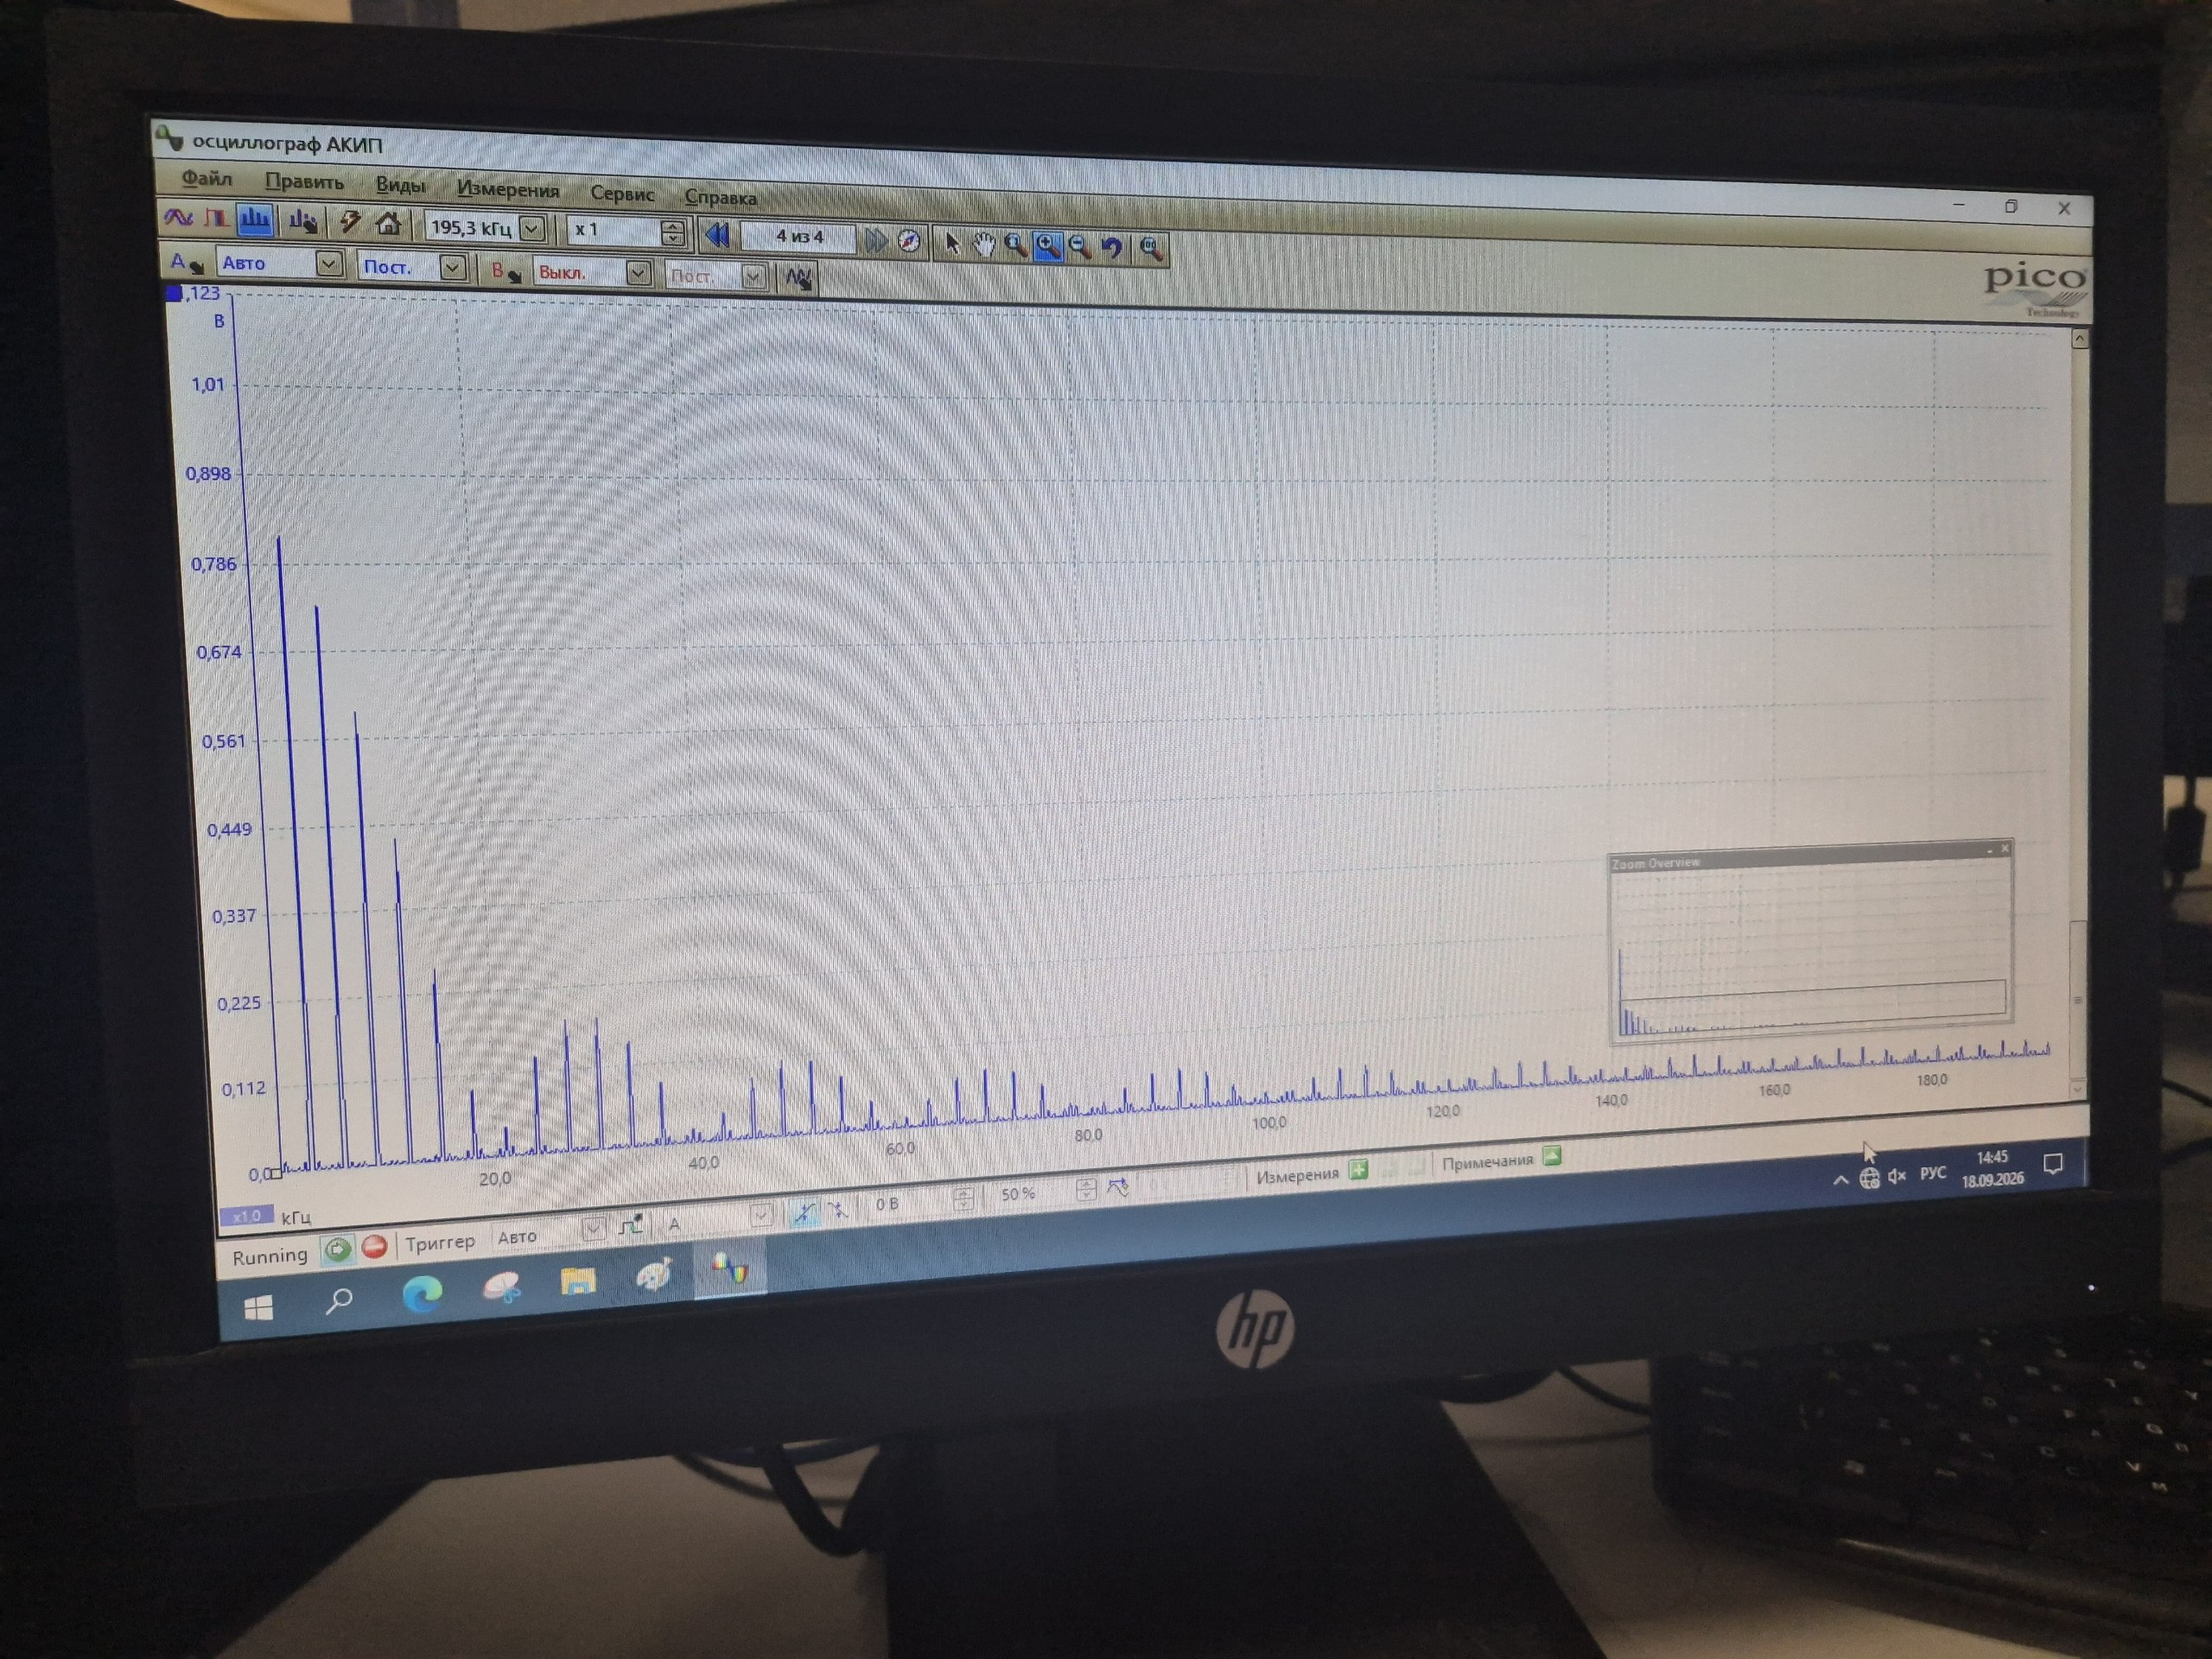
\includegraphics[width=\textwidth]{images/A_3kHz.jpg}
        \caption{$\nu_{\text{повт}}=3$ кГц}
    \end{subfigure}
    \hfill
    \begin{subfigure}{0.48\textwidth}
        \centering
        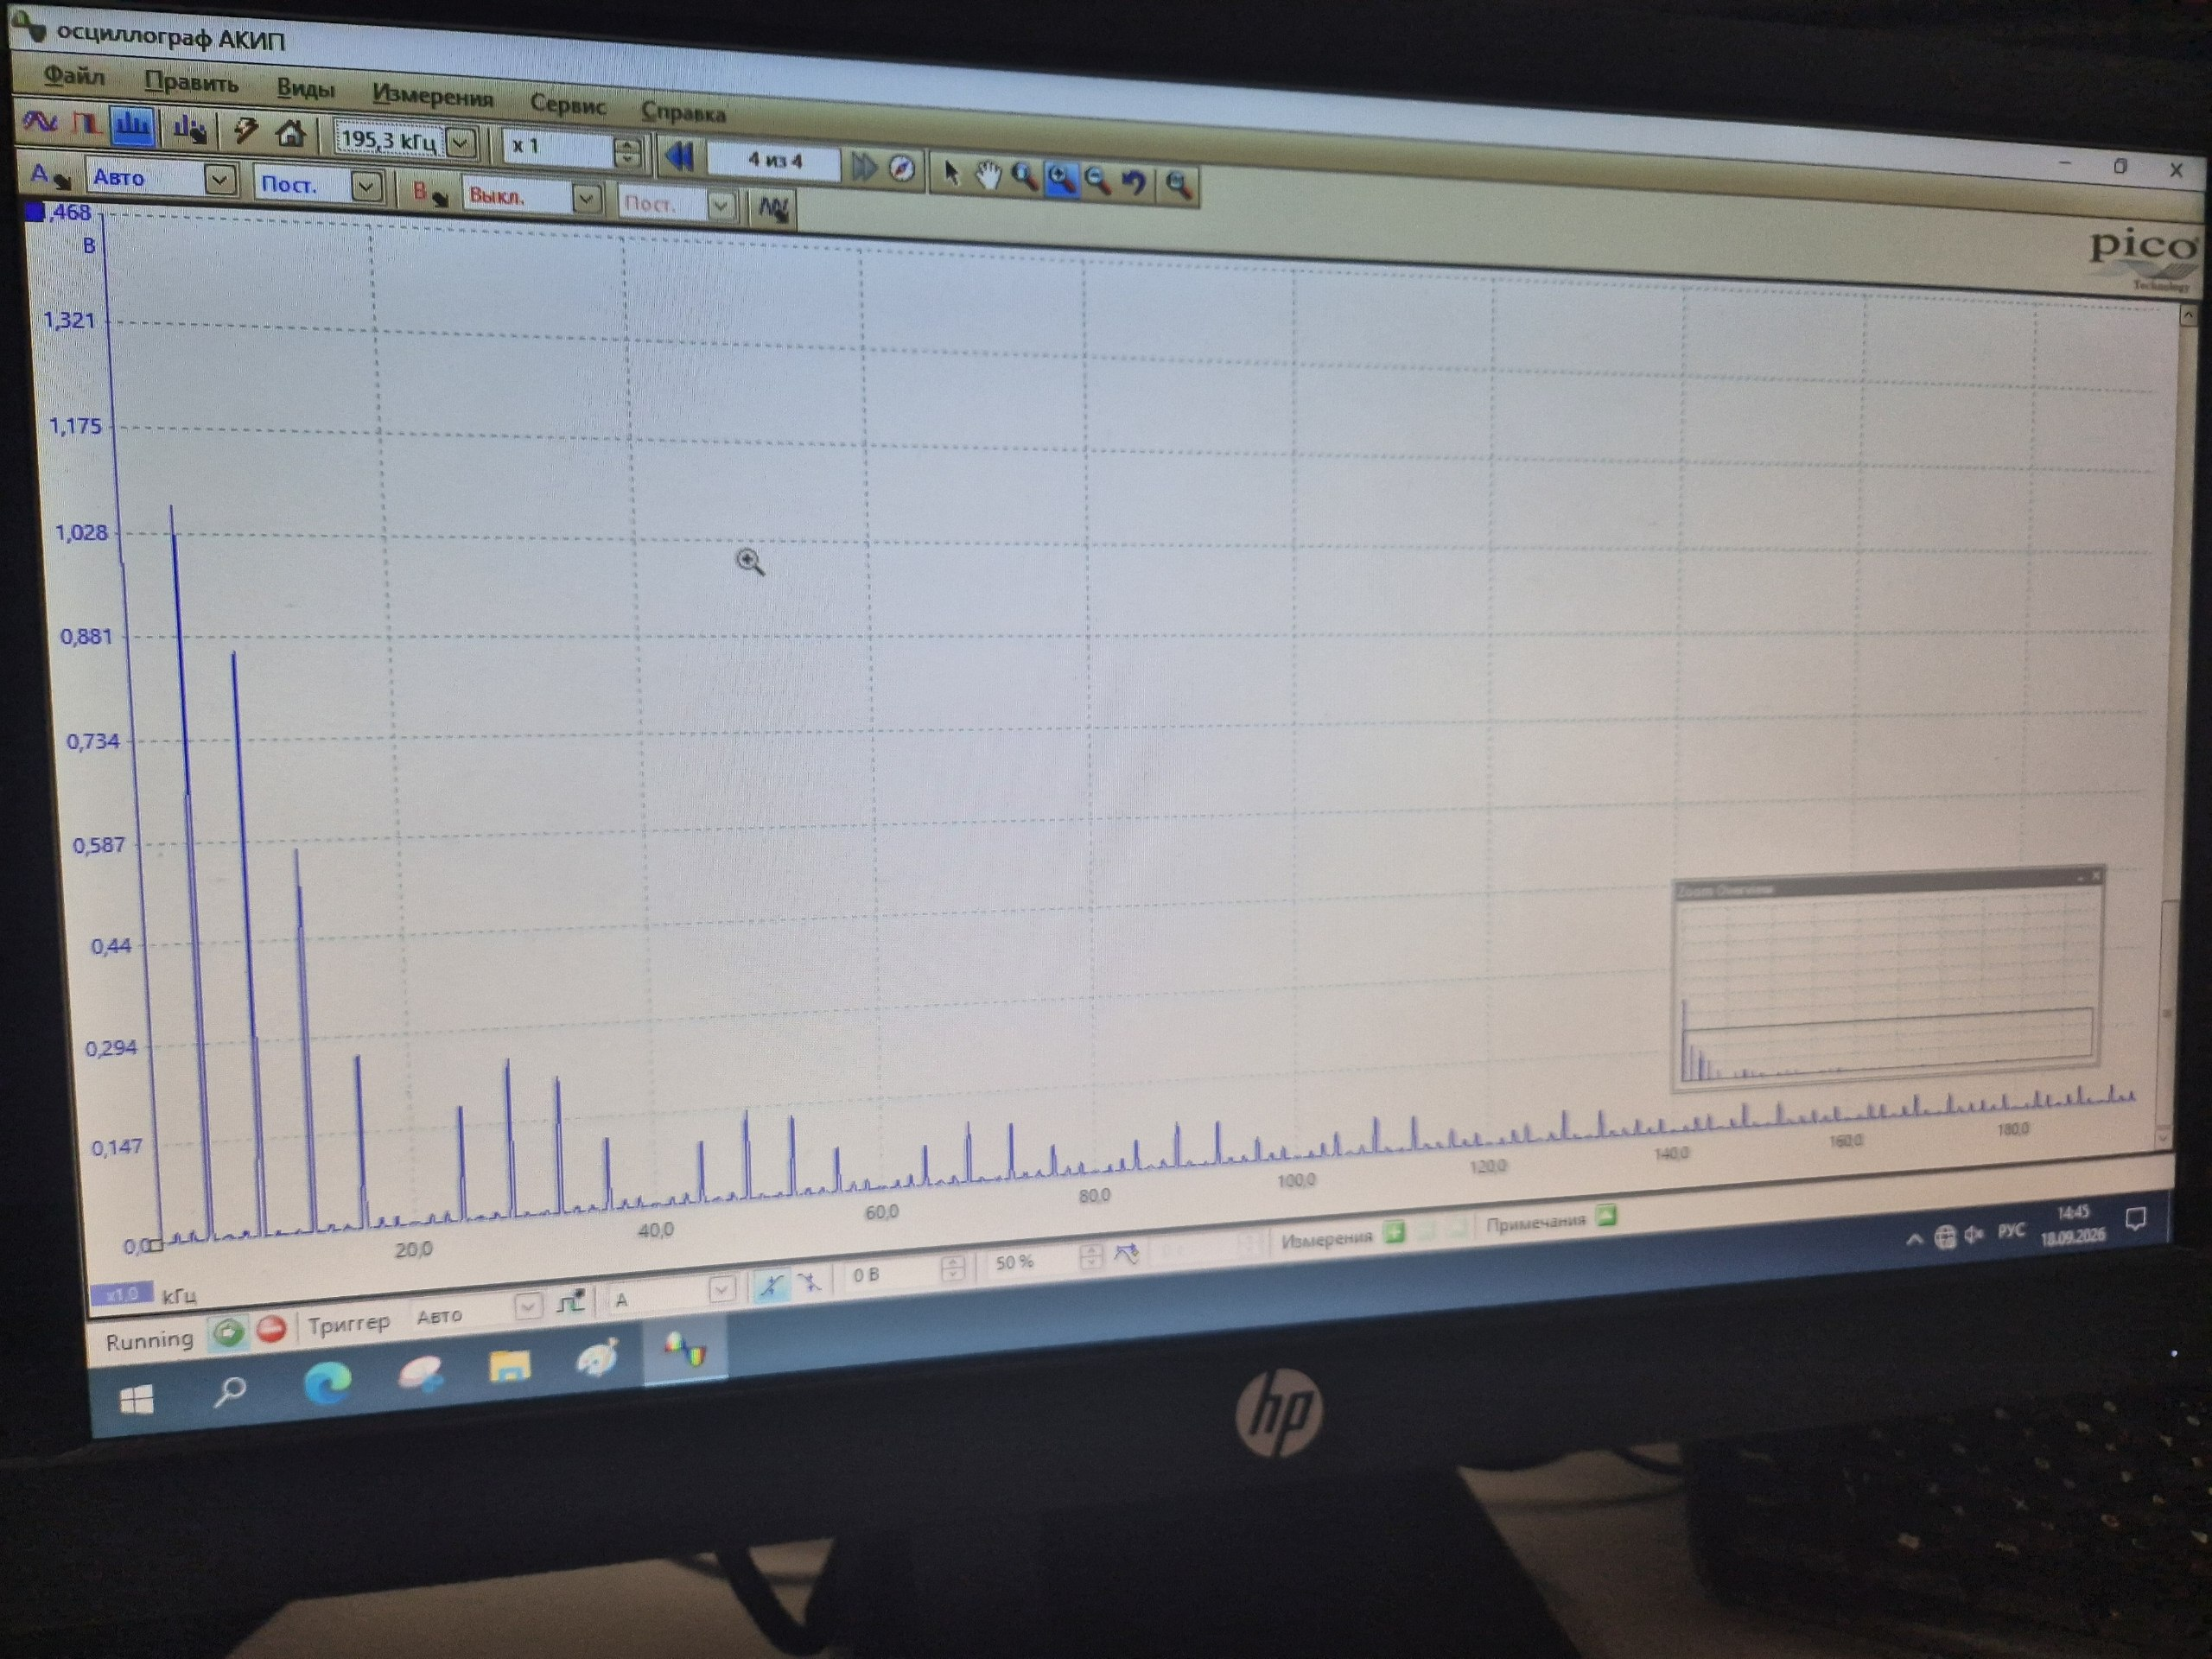
\includegraphics[width=\textwidth]{images/A_4kHz.jpg}
        \caption{$\nu_{\text{повт}}=4$ кГц}
    \end{subfigure}

    \caption{Изменение спектра при изменении частоты повторения
    импульсов при $\tau=50$ мкс}
    \label{fig:A_freq}
\end{figure}

Как видно из графиков, при увеличении частоты повторения сигнала увеличивается расстояние между компонентами спектра.

Во втором исследовании частота повторения оставалась постоянной:
\[
\nu_{\text{повт}}=1~\text{кГц},
\]
а длительность импульса изменялась от $50$ до $200$ мкс.

\begin{figure}[H]
    \centering

    \begin{subfigure}{0.48\textwidth}
        \centering
        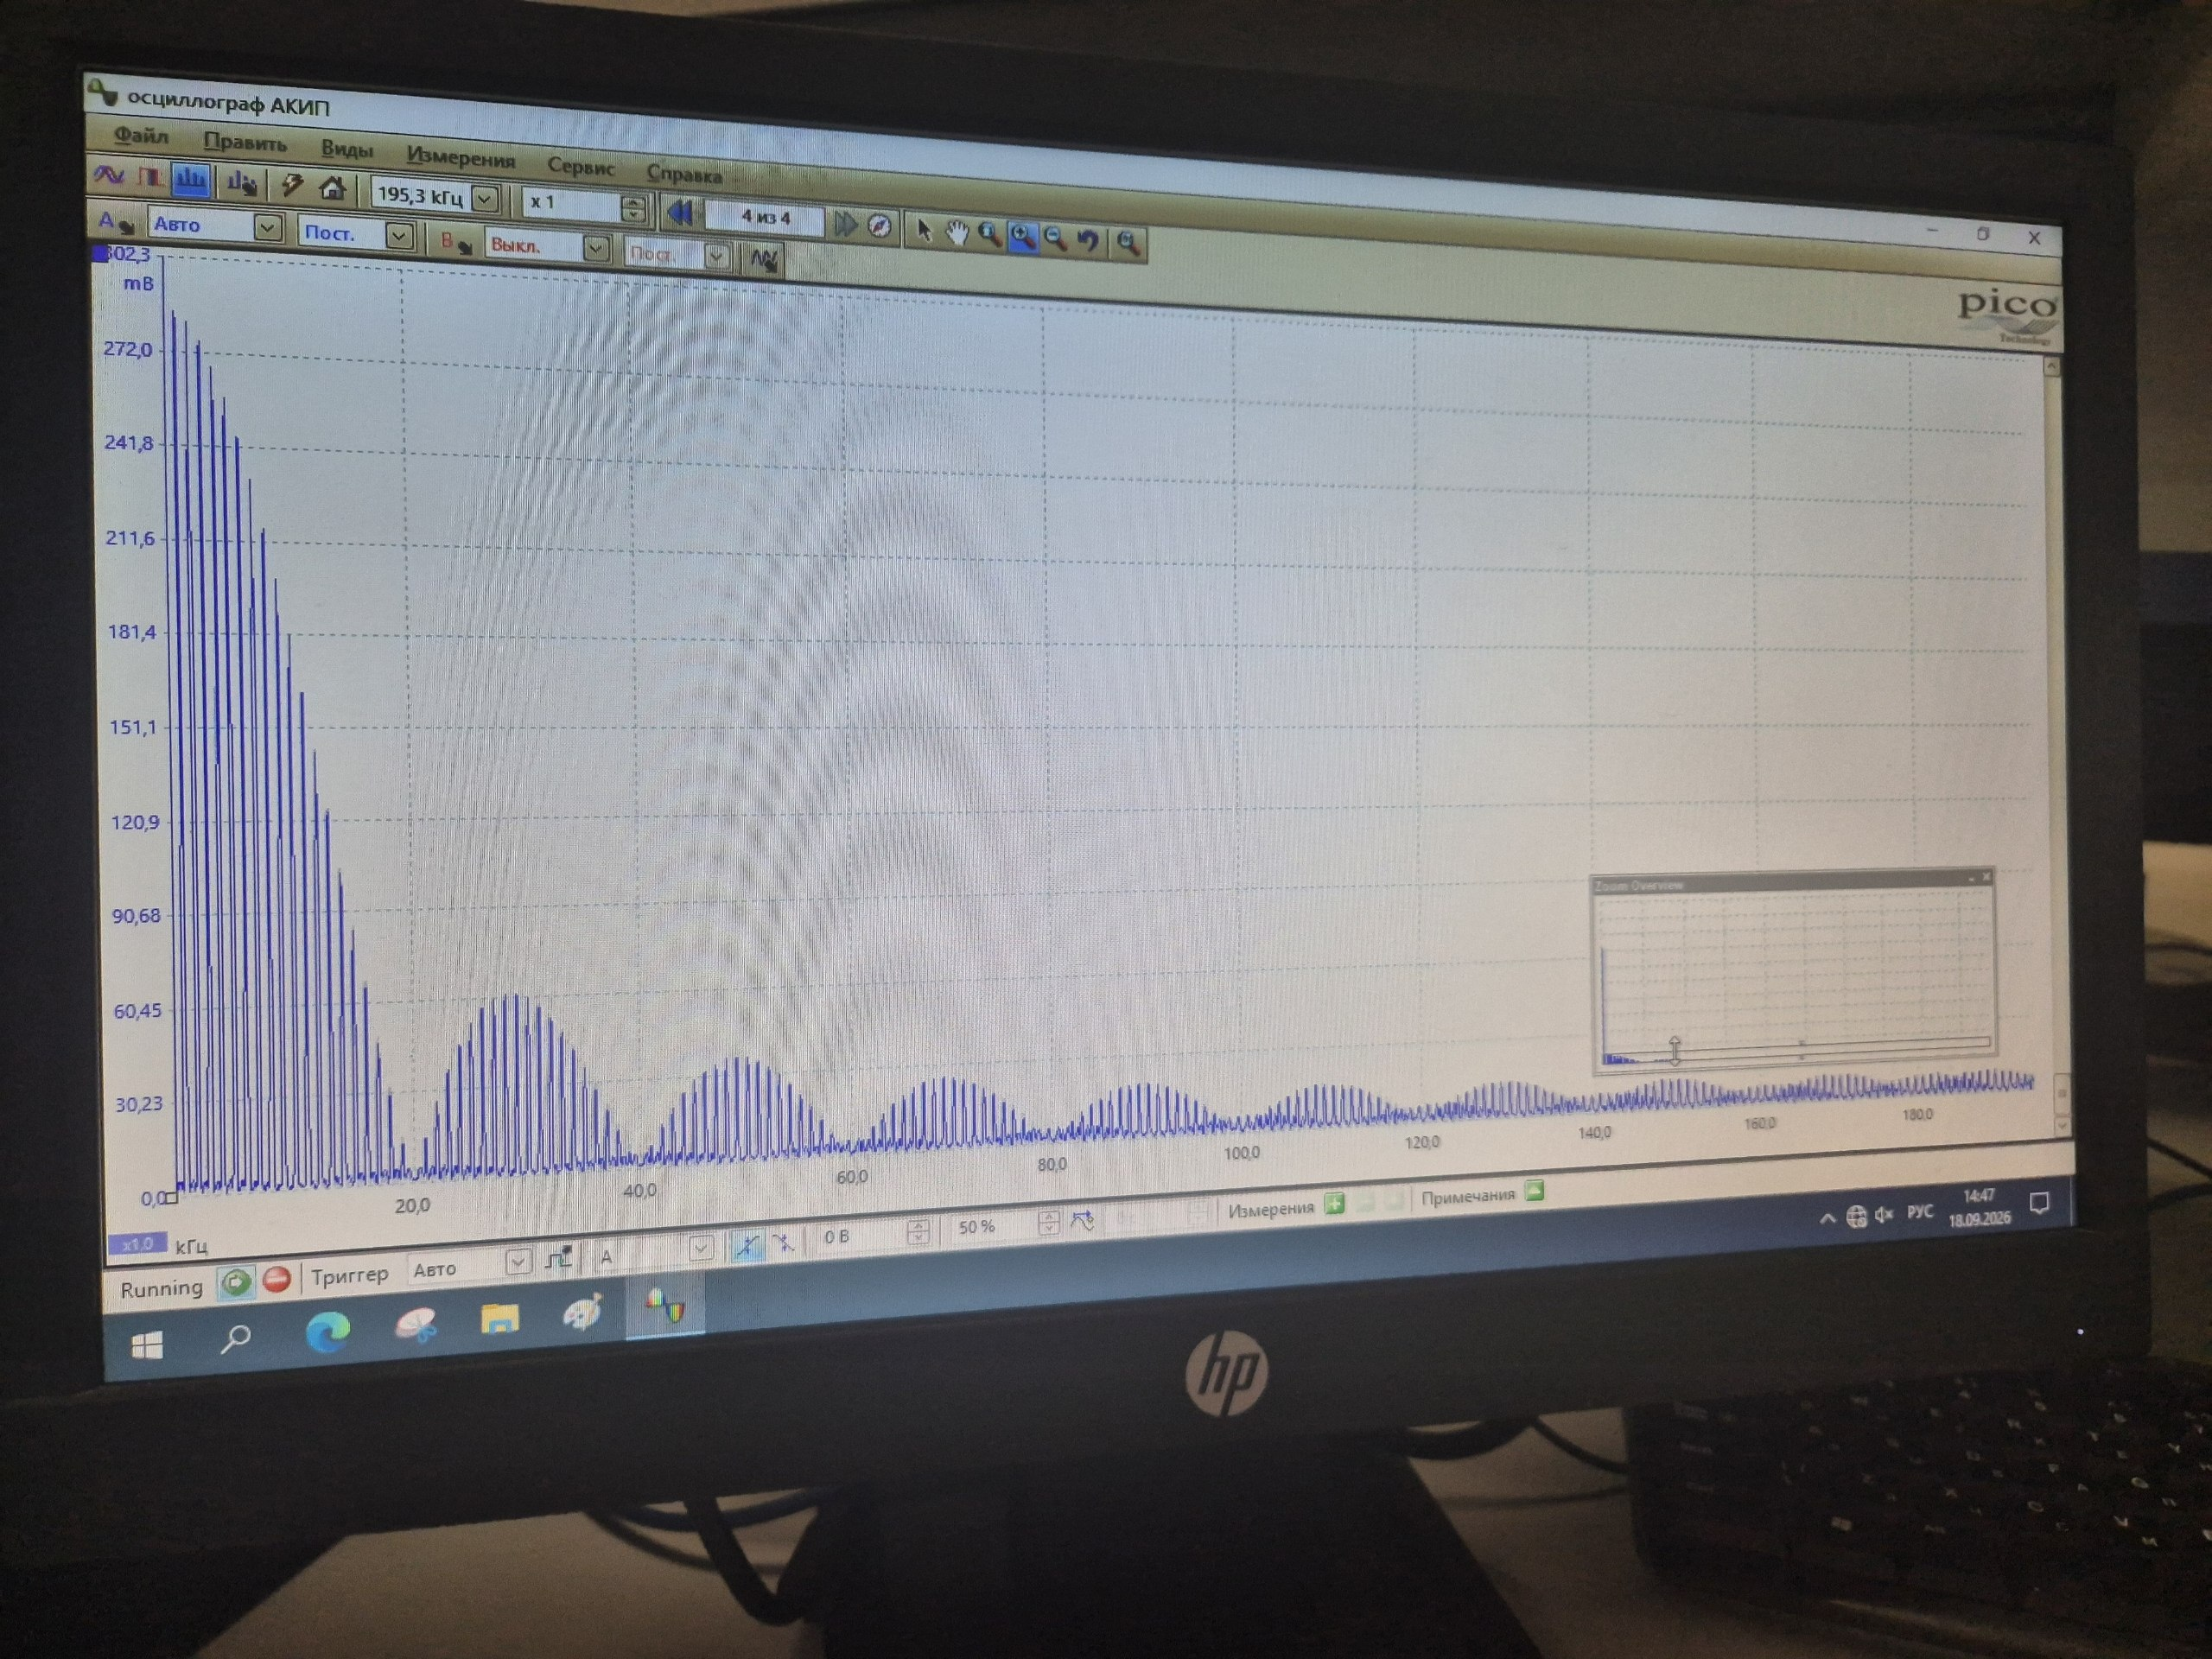
\includegraphics[width=\textwidth]{images/A_50us.jpg}
        \caption{$\tau=50$ мкс}
    \end{subfigure}
    \hfill
    \begin{subfigure}{0.48\textwidth}
        \centering
        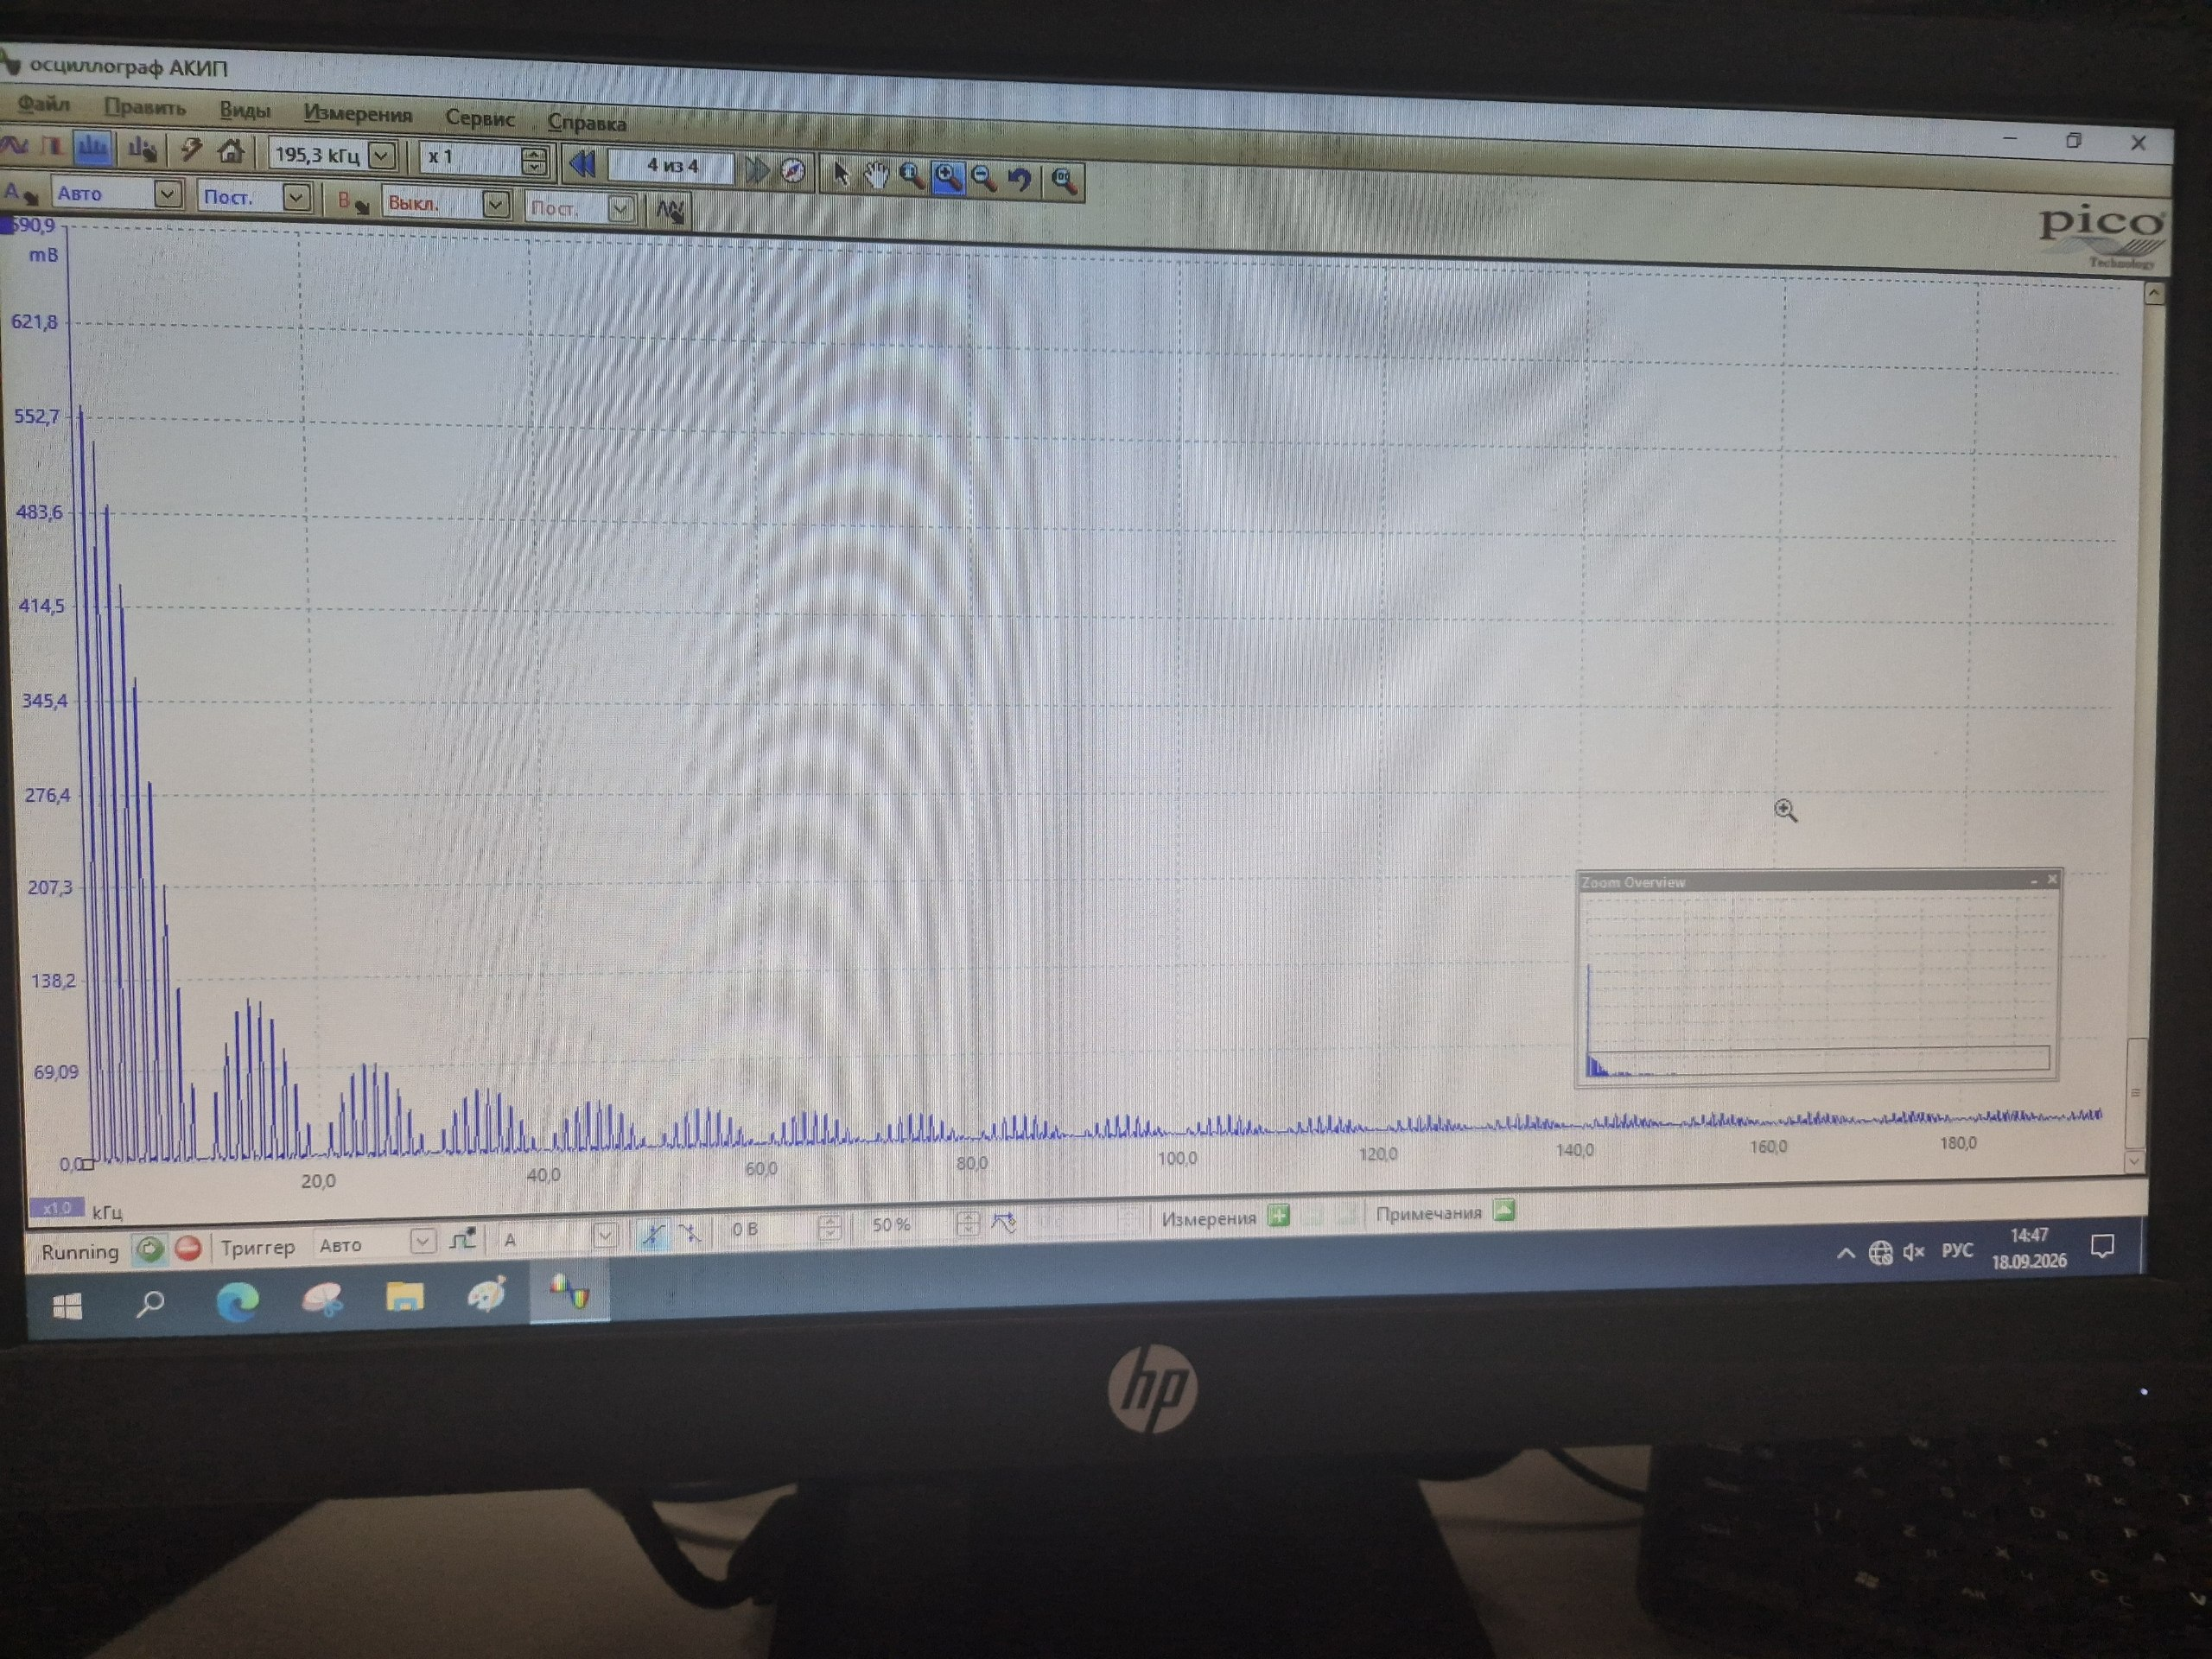
\includegraphics[width=\textwidth]{images/A_100us.jpg}
        \caption{$\tau=100$ мкс}
    \end{subfigure}

    \vspace{0.5cm}

    \begin{subfigure}{0.48\textwidth}
        \centering
        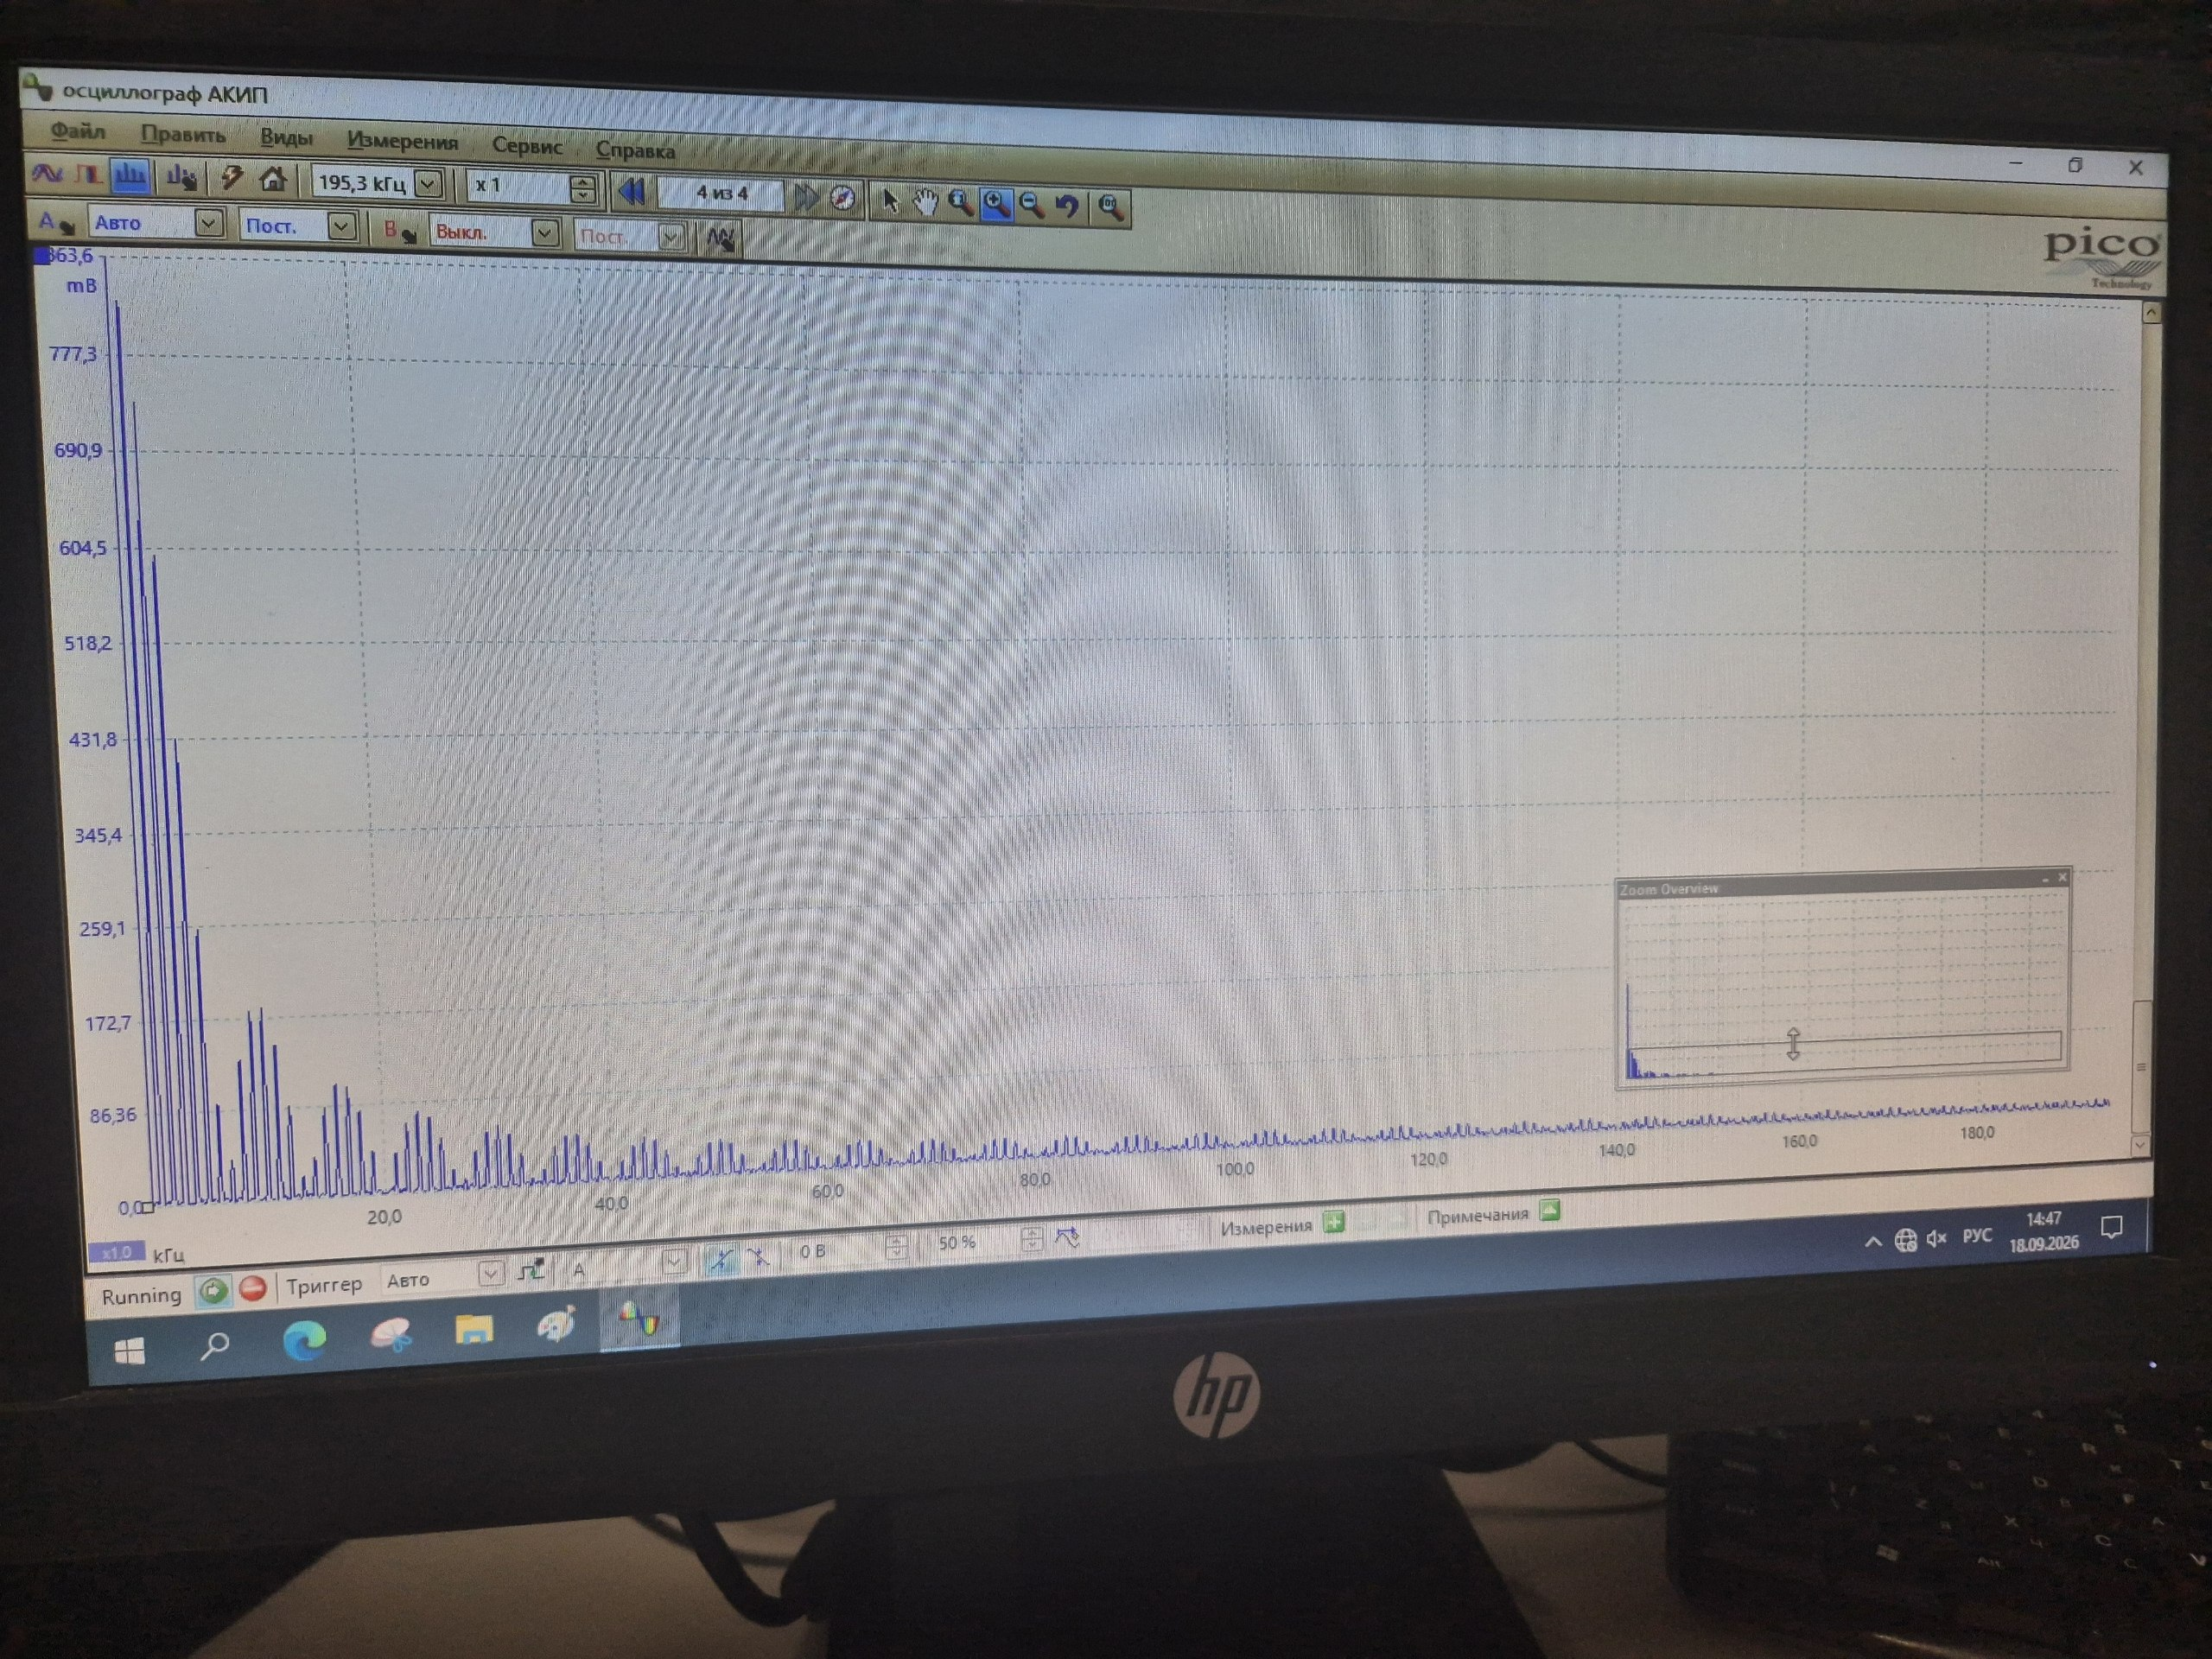
\includegraphics[width=\textwidth]{images/A_150us.jpg}
        \caption{$\tau=150$ мкс}
    \end{subfigure}
    \hfill
    \begin{subfigure}{0.48\textwidth}
        \centering
        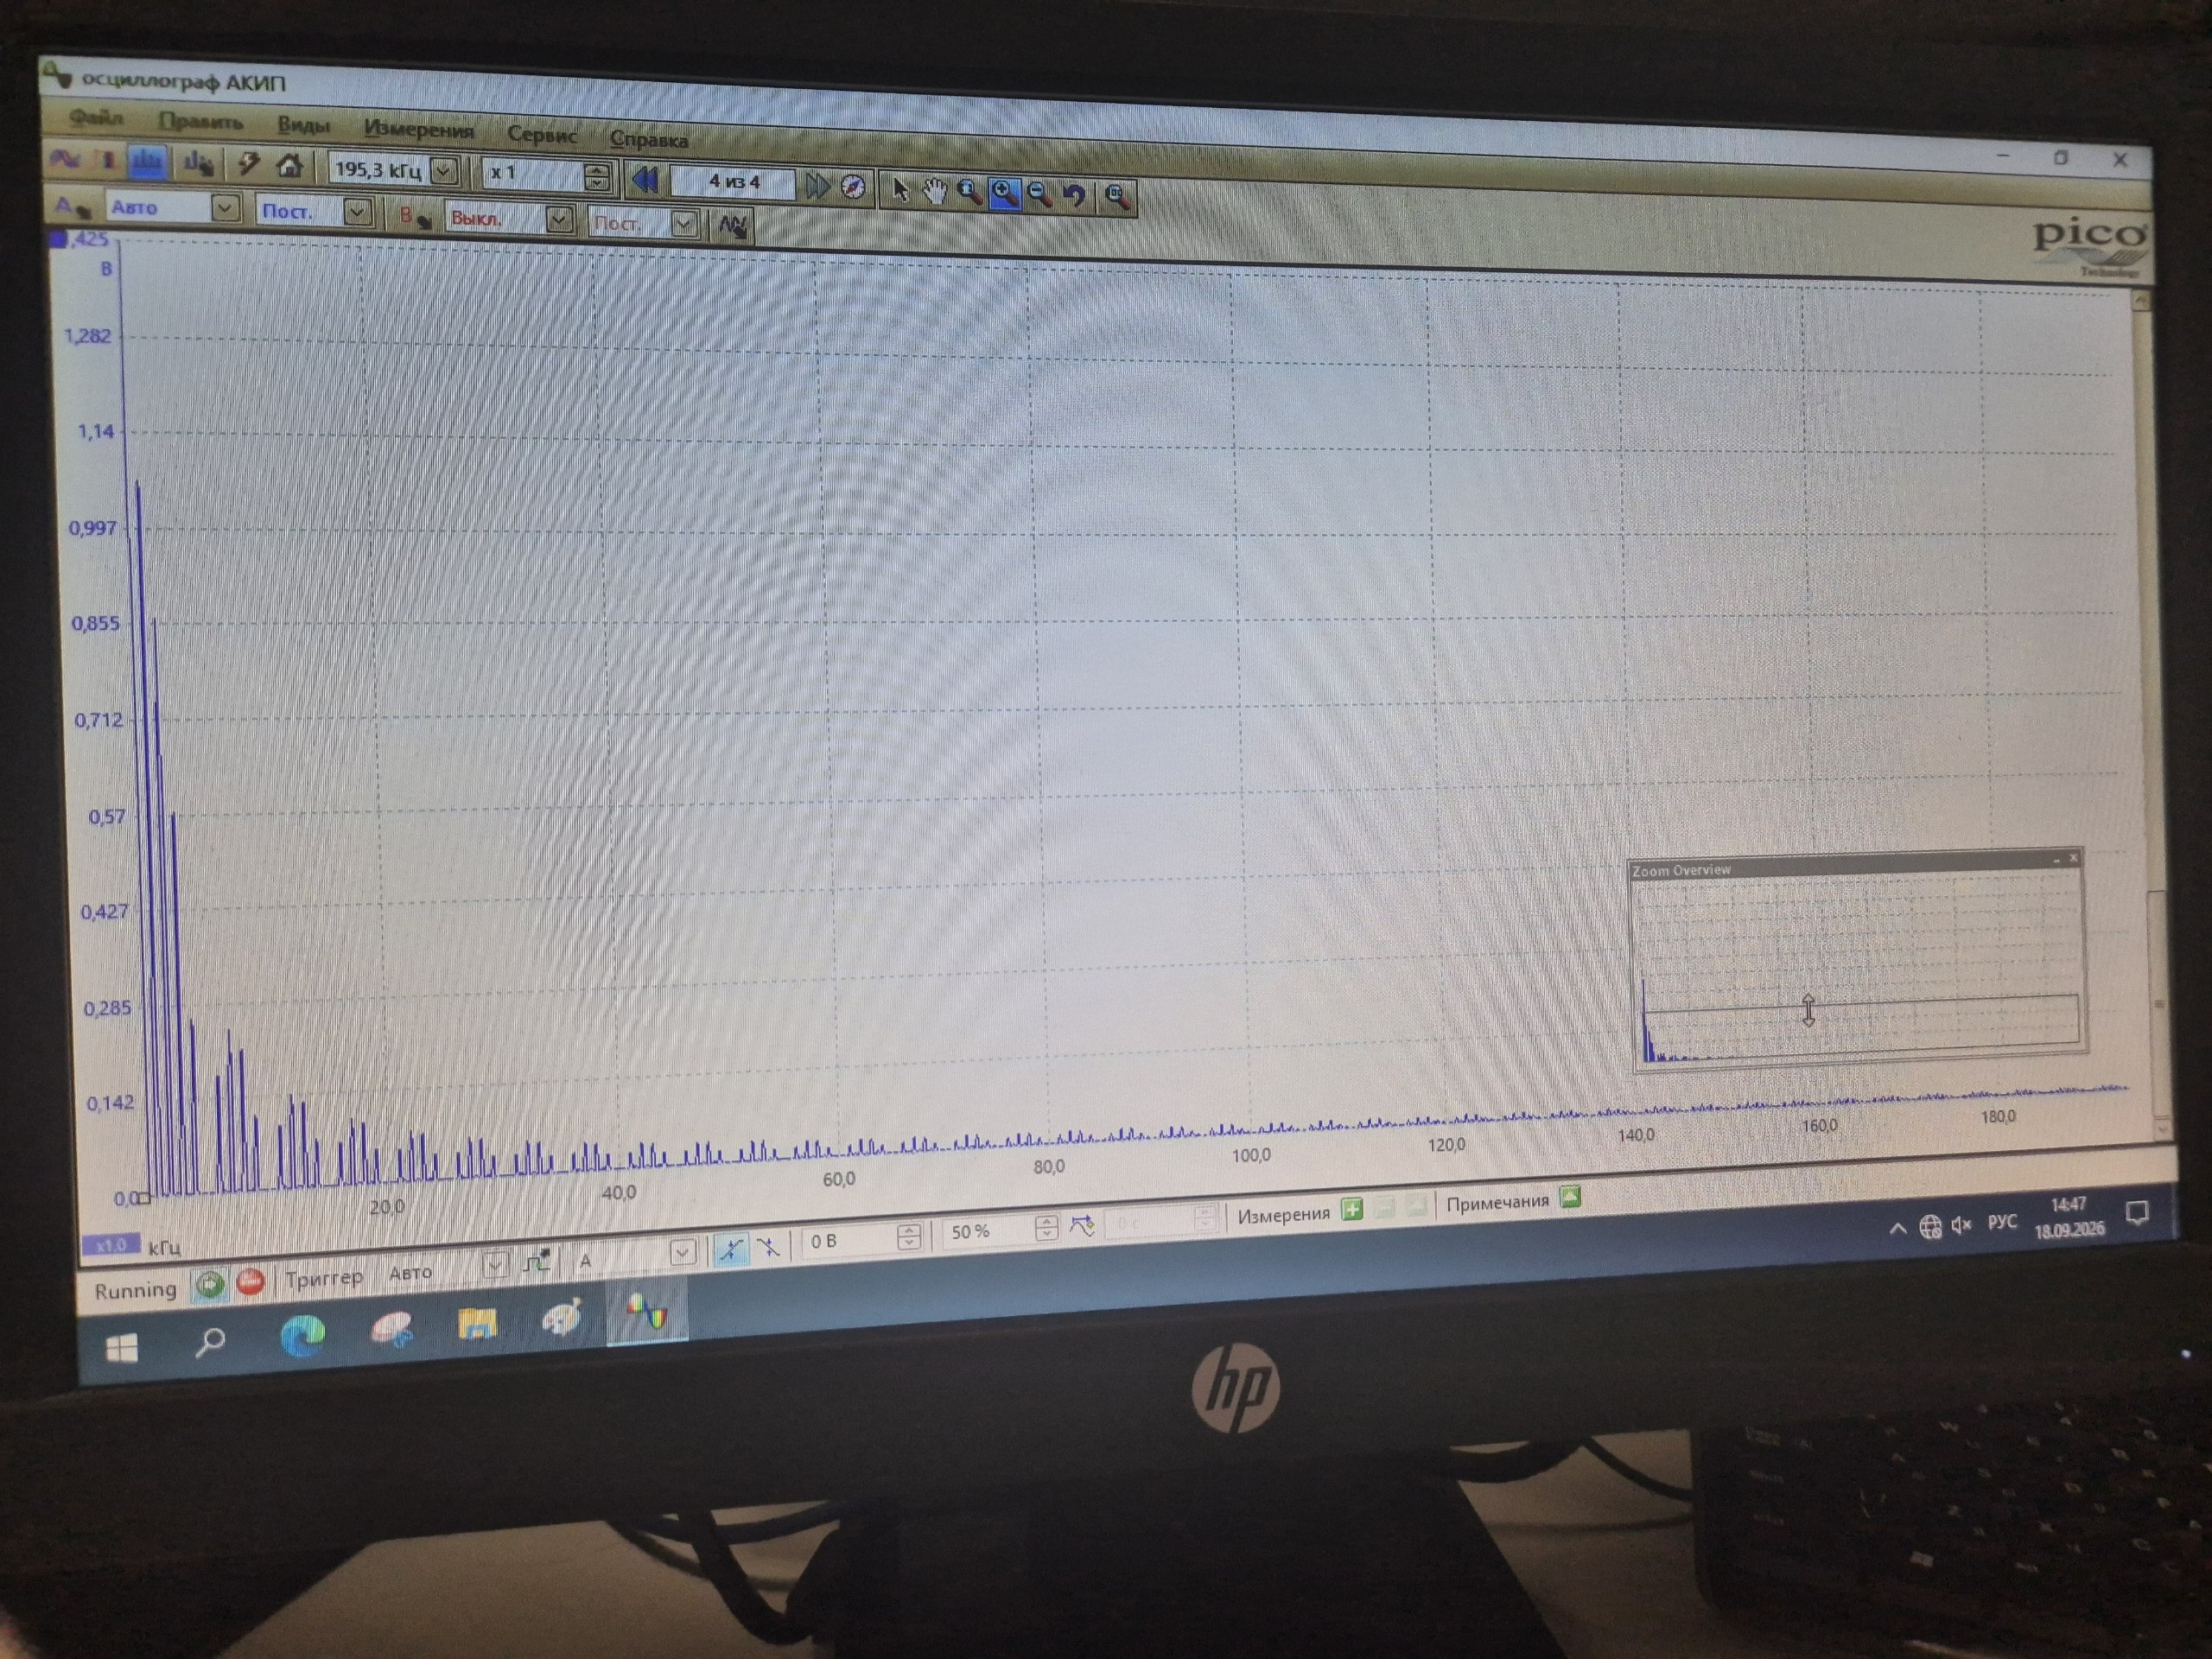
\includegraphics[width=\textwidth]{images/A_200us.jpg}
        \caption{$\tau=200$ мкс}
    \end{subfigure}

    \caption{Изменение спектра при изменении длительности импульса
    при $\nu_{\text{повт}}=1$ кГц}
    \label{fig:A_tau}
\end{figure}

Как видно из графиков, при увеличении длительности сигнала уменьшается ширина спектра.

\subsection{Измерение спектральных компонент}

Измерялись частоты и амплитуды нескольких спектральных гармоник.

Теоретически:
\begin{equation}
\nu_n=\frac{n}{T},
\end{equation}

\begin{equation}
|a_n|=
\frac{\tau}{T}
\frac{|\sin(\pi\nu_n\tau)|}
{\pi\nu_n\tau}.
\end{equation}

% TODO: заполнить после обработки измерений

\begin{table}[H]
\centering
\caption{Экспериментальные и теоретические значения спектральных компонент}
\begin{tabular}{c|cccccccc}
$n$ & 1 & 2 & 3 & 4 & 5 & 6 & 7 & 8 \\
\hline
$\nu_n^{\text{эксп}}$, Гц
& 0.96 & 2.02 & 2.96 & 3.98 & 5.00 & 5.99 & 7.05 & 7.99 \\
$\nu_n^{\text{теор}}$, Гц
& 1 & 2 & 3 & 4 & 5 & 6 & 7 & 8 \\
$|a_n|^{\text{эксп}}$
& 283.9 & 280.2 & 282.8 & 265.9 & 256.0 & 242.9 & 229.3 & 215.0 \\
$|a_n/a_1|^{\text{эксп}}$
& 1.000 & 0.987 & 0.996 & 0.937 & 0.902 & 0.856 & 0.808 & 0.757 \\
$|a_n/a_1|^{\text{теор}}$
& 1.000 & 0.988 & 0.967 & 0.939 & 0.904 & 0.862 & 0.814 & 0.760
\end{tabular}
\end{table}

\subsection{Проверка соотношений неопределённостей}

При фиксированном периоде $T$ исследовалась зависимость ширины спектра
$\Delta\nu$ от длительности импульса $\tau$.

\begin{table}[H]
\centering
\caption{Зависимость ширины спектра от длительности импульса}
\begin{tabular}{c|c|c}
$\tau$, мкс & $1/\tau$, кГц & $\Delta\nu$, кГц \\
\hline
20 & 50.00 & 48.62\\
40 & 25.00 & 24.93\\
60 & 16.67 & 16.44\\
80 & 12.50 & 12.52\\
100 & 10.00 & 9.95\\
120 & 8.33 & 7.61\\
140 & 7.14 & 6.71\\
160 & 6.25 & 5.50\\
180 & 5.56 & 5.19\\
200 & 5.00 & 4.93 
\end{tabular}
\end{table}

% TODO: график Delta nu(1/tau)

\begin{figure}[H]
    \centering
    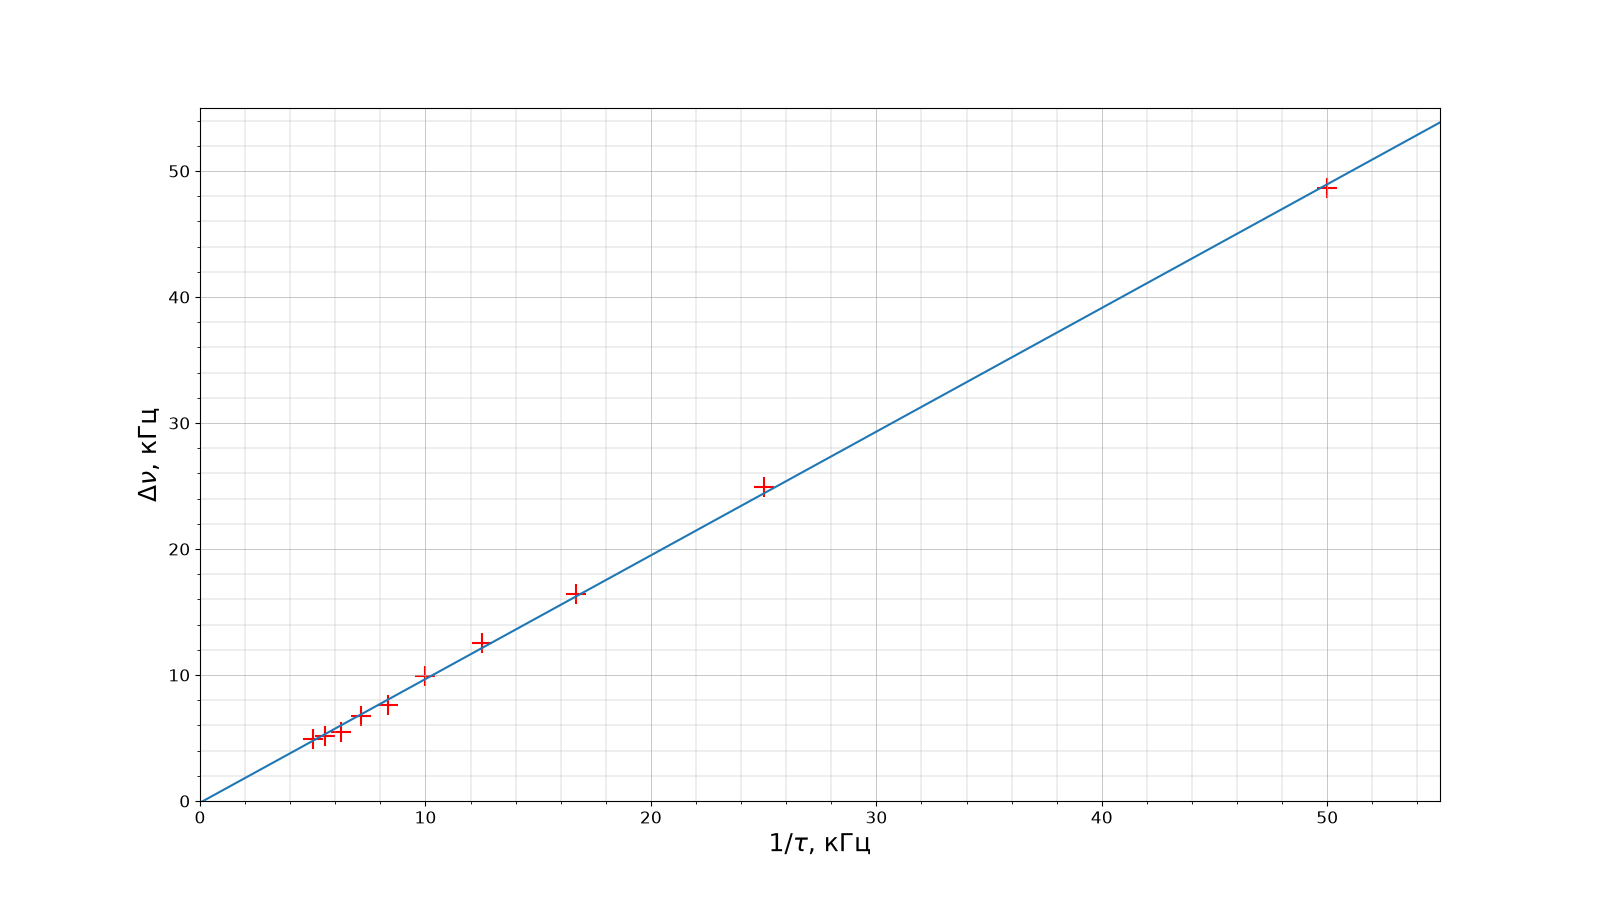
\includegraphics[width=1\textwidth]{images/delta_nu_1_tau.png}
    \caption{Зависимость ширины спектра $\Delta\nu$ от обратной длительности импульса $1/\tau$.}
    \label{fig:delta_nu_1_tau}
\end{figure}

Из графика получено:
\[
\Delta\nu = (0{,}982 \pm 0{,}009)\frac{1}{\tau}
-(0{,}137 \pm 0{,}180).
\]

Следовательно,
\[
\Delta\nu\,\tau \approx 0{,}982.
\]

Таким образом, эксперимент подтверждает соотношение неопределённостей
\[
\Delta\nu\,\tau \sim 1.
\]

\vspace{4cm}

При фиксированной длительности импульса $\tau$ исследовалась зависимость
расстояния между соседними гармониками $\delta\nu$ от $1/T$.

\begin{table}[H]
\centering
\caption{Зависимость расстояния между гармониками от периода}
\begin{tabular}{c|c|c}
$T$, мкс & $1/T$, кГц & $\delta\nu$, кГц \\
\hline
200 & 5.00 & 4.98 \\
800 & 1.25 & 1.32\\
1400 & 0.714 & 0.72\\
2000 & 0.500 & 0.47 \\
2600 & 0.385 & 0.40 \\
3200 & 0.313 & 0.31 \\
3800 & 0.263 & 0.27 \\
4400 & 0.227 & 0.22 \\
5000 & 0.200 & 0.20 
\end{tabular}
\end{table}

% TODO: график delta nu(1/T)

\begin{figure}[H]
    \centering
    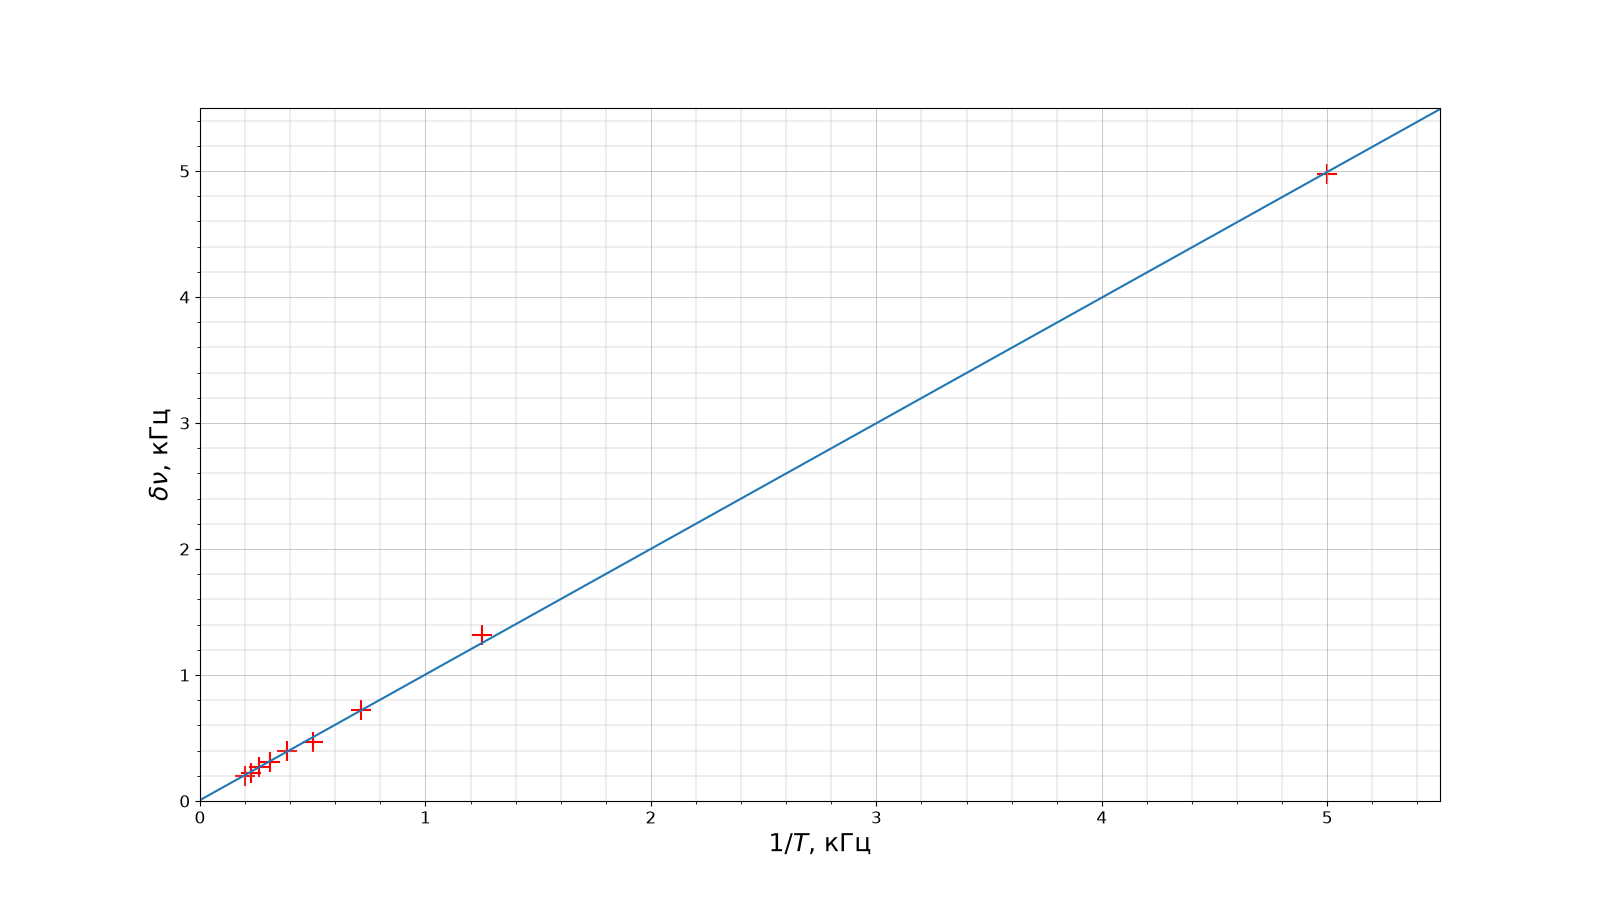
\includegraphics[width=0.9\textwidth]{images/delta_nu_1_T.png}
    \caption{Зависимость расстояния между соседними гармониками $\delta\nu$ от обратного периода $1/T$.}
\end{figure}

Из графика получено:
\[
\delta\nu=(0{.}997\pm0{.}007)\frac{1}{T}
+(0{.}007\pm0{.}012).
\]

Коэффициент наклона экспериментальной зависимости
\[
a=0{,}997\pm0{,}007
\]
согласуется с теоретическим значением $a=1$.

Таким образом, эксперимент подтверждает соотношение
\[
\boxed{\delta\nu=\frac{1}{T}},
\]
то есть справедливость соответствующего соотношения неопределённости.

% =========================================================
% Б
% =========================================================

\section{Наблюдение спектра периодической последовательности цугов}

\subsection{Параметры сигнала}

Исследовалась периодическая последовательность импульсов синусоидальной
формы (цугов).

% TODO: вписать фактические параметры

\begin{table}[H]
\centering
\caption{Параметры последовательности цугов}
\begin{tabular}{|c|c|}
\hline
Параметр & Значение \\
\hline
$\nu_0$ & 50 кГц\\
\hline
$T$ & 1 мс\\
\hline
$N$ & 5\\
\hline
$\tau$ & 100 мкс\\
\hline
\end{tabular}
\end{table}

\subsection{Наблюдение спектра}

При исследовании спектра периодической последовательности цугов
изменялись число периодов в цуге $N$, период повторения $T$ и частота
заполнения $\nu_0$.

\newpage

\subsubsection*{Изменение числа периодов в цуге}

Были получены спектры при изменении числа периодов в цуге
от $N=5$ до $N=20$.

\begin{figure}[H]
    \centering

    \begin{subfigure}{0.48\textwidth}
        \centering
        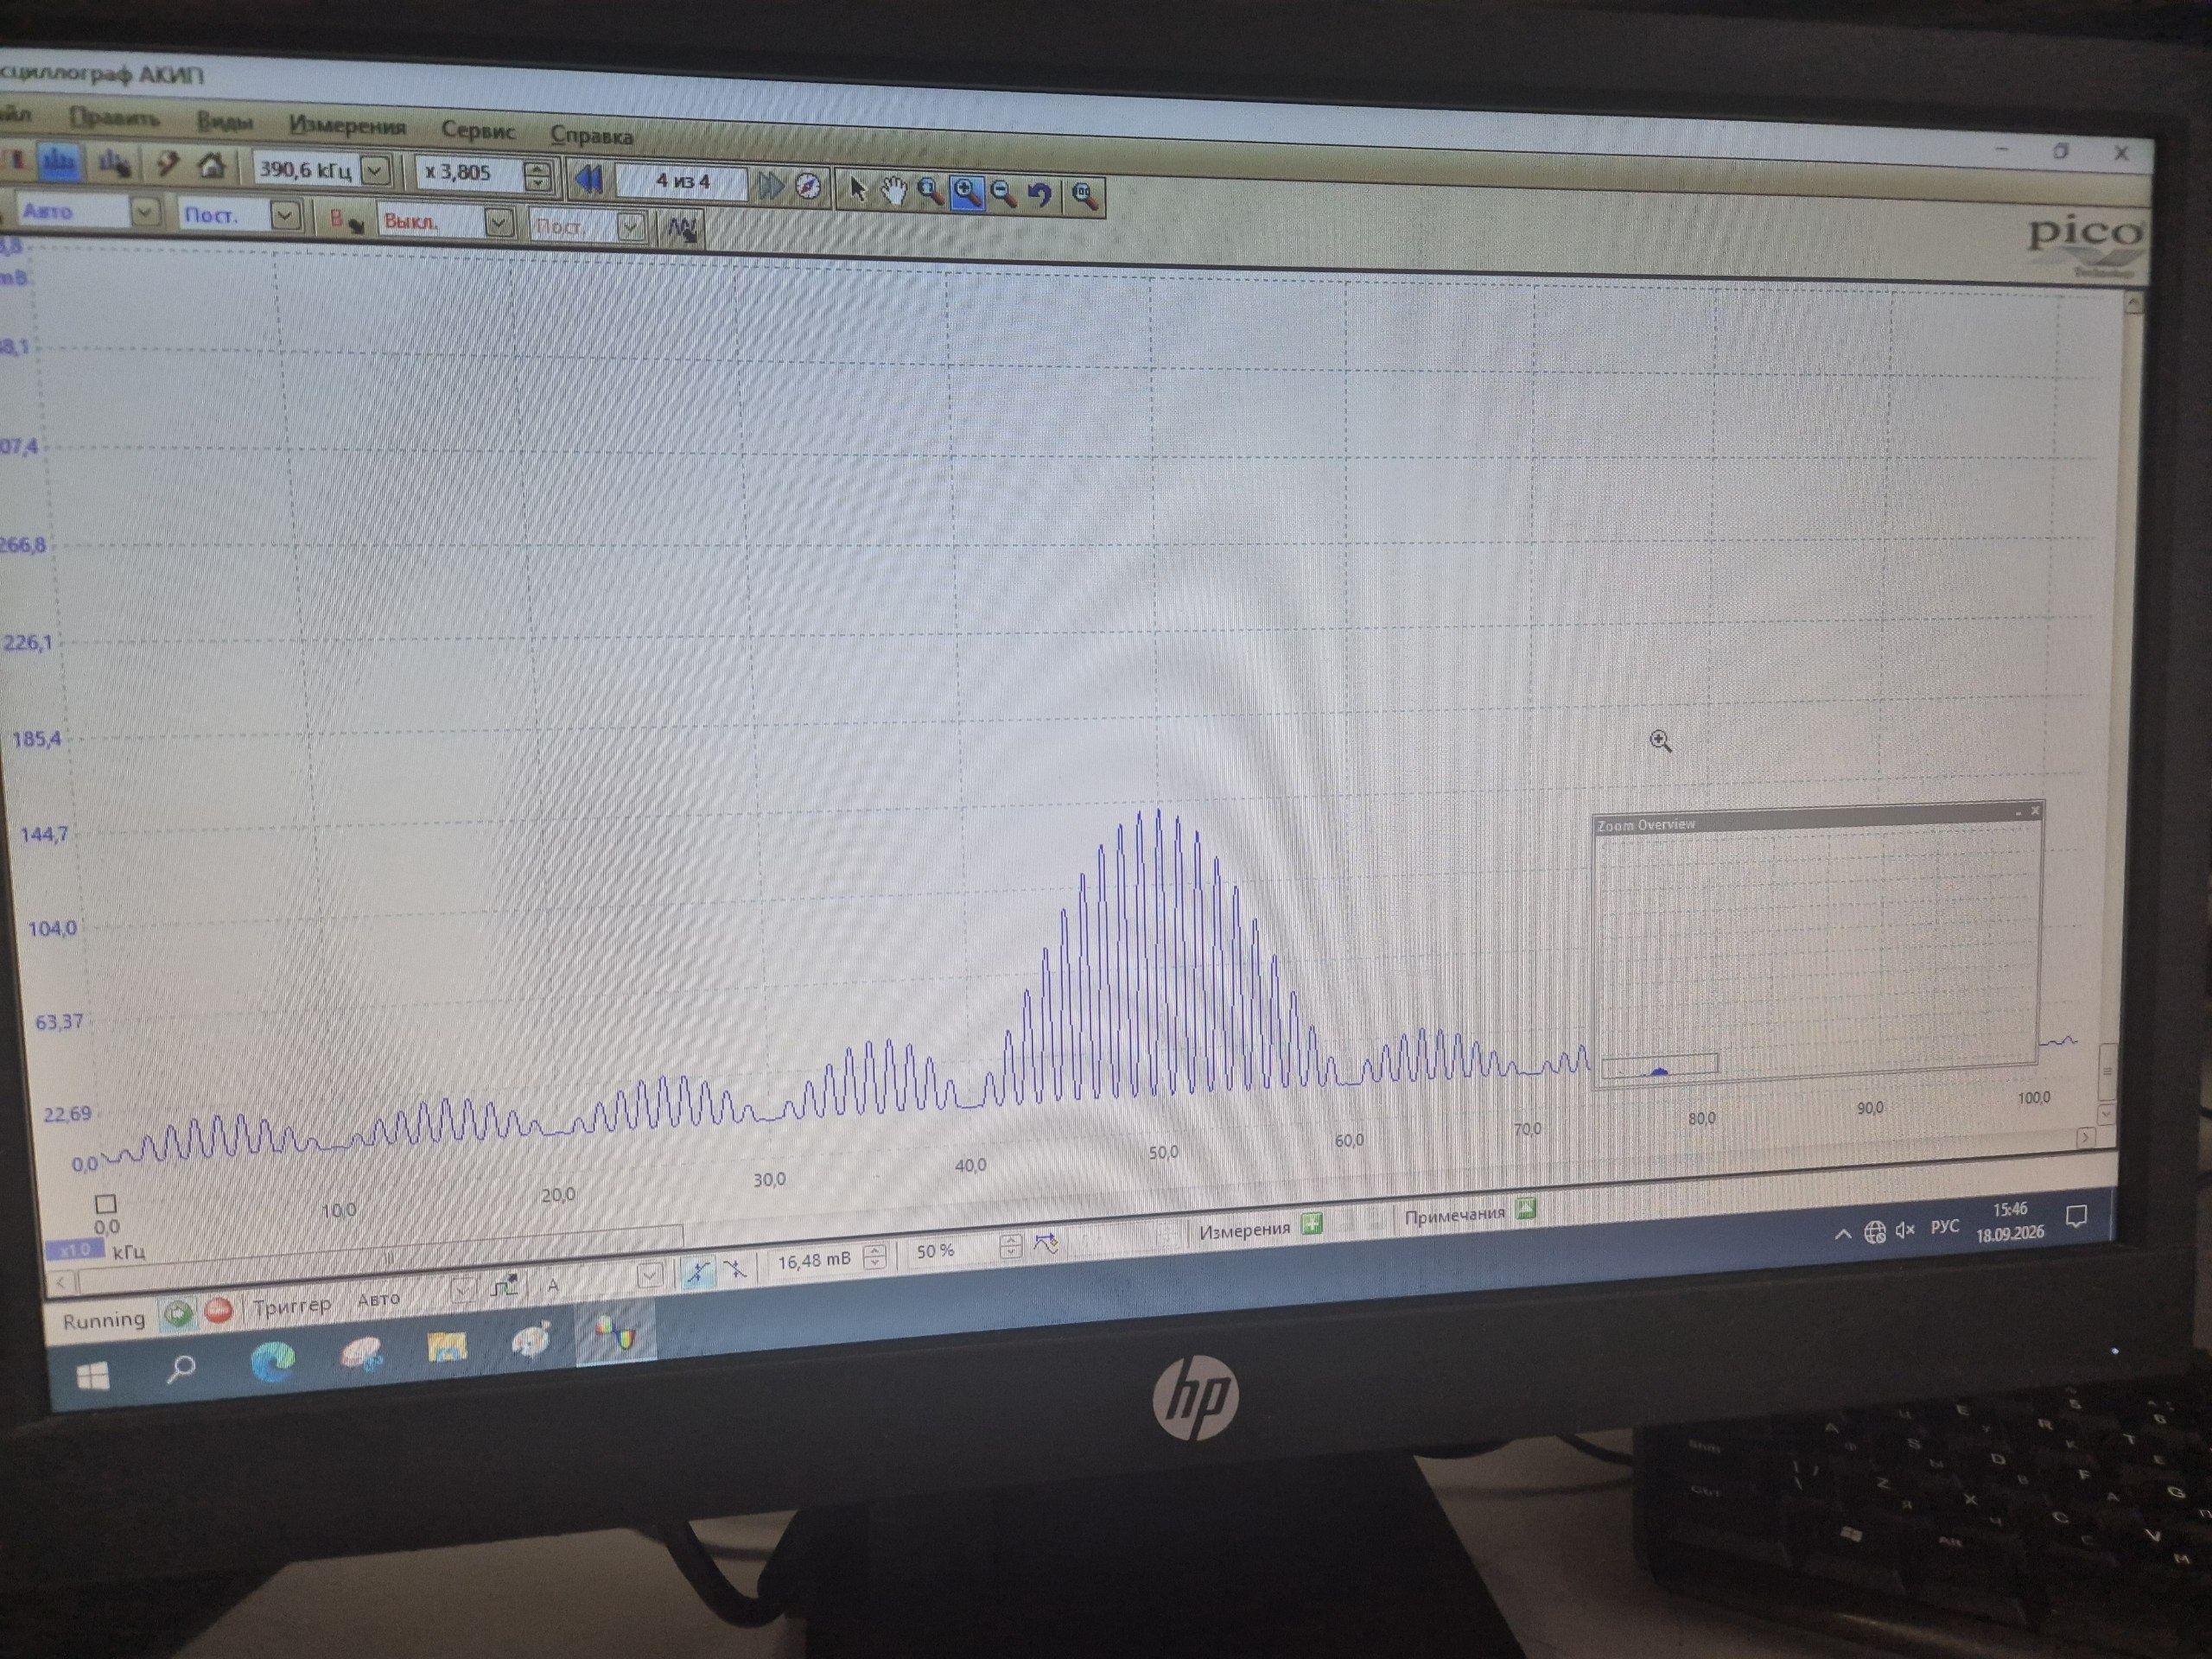
\includegraphics[width=\textwidth]{images/B_N5.jpg}
        \caption{$N=5$}
    \end{subfigure}
    \hfill
    \begin{subfigure}{0.48\textwidth}
        \centering
        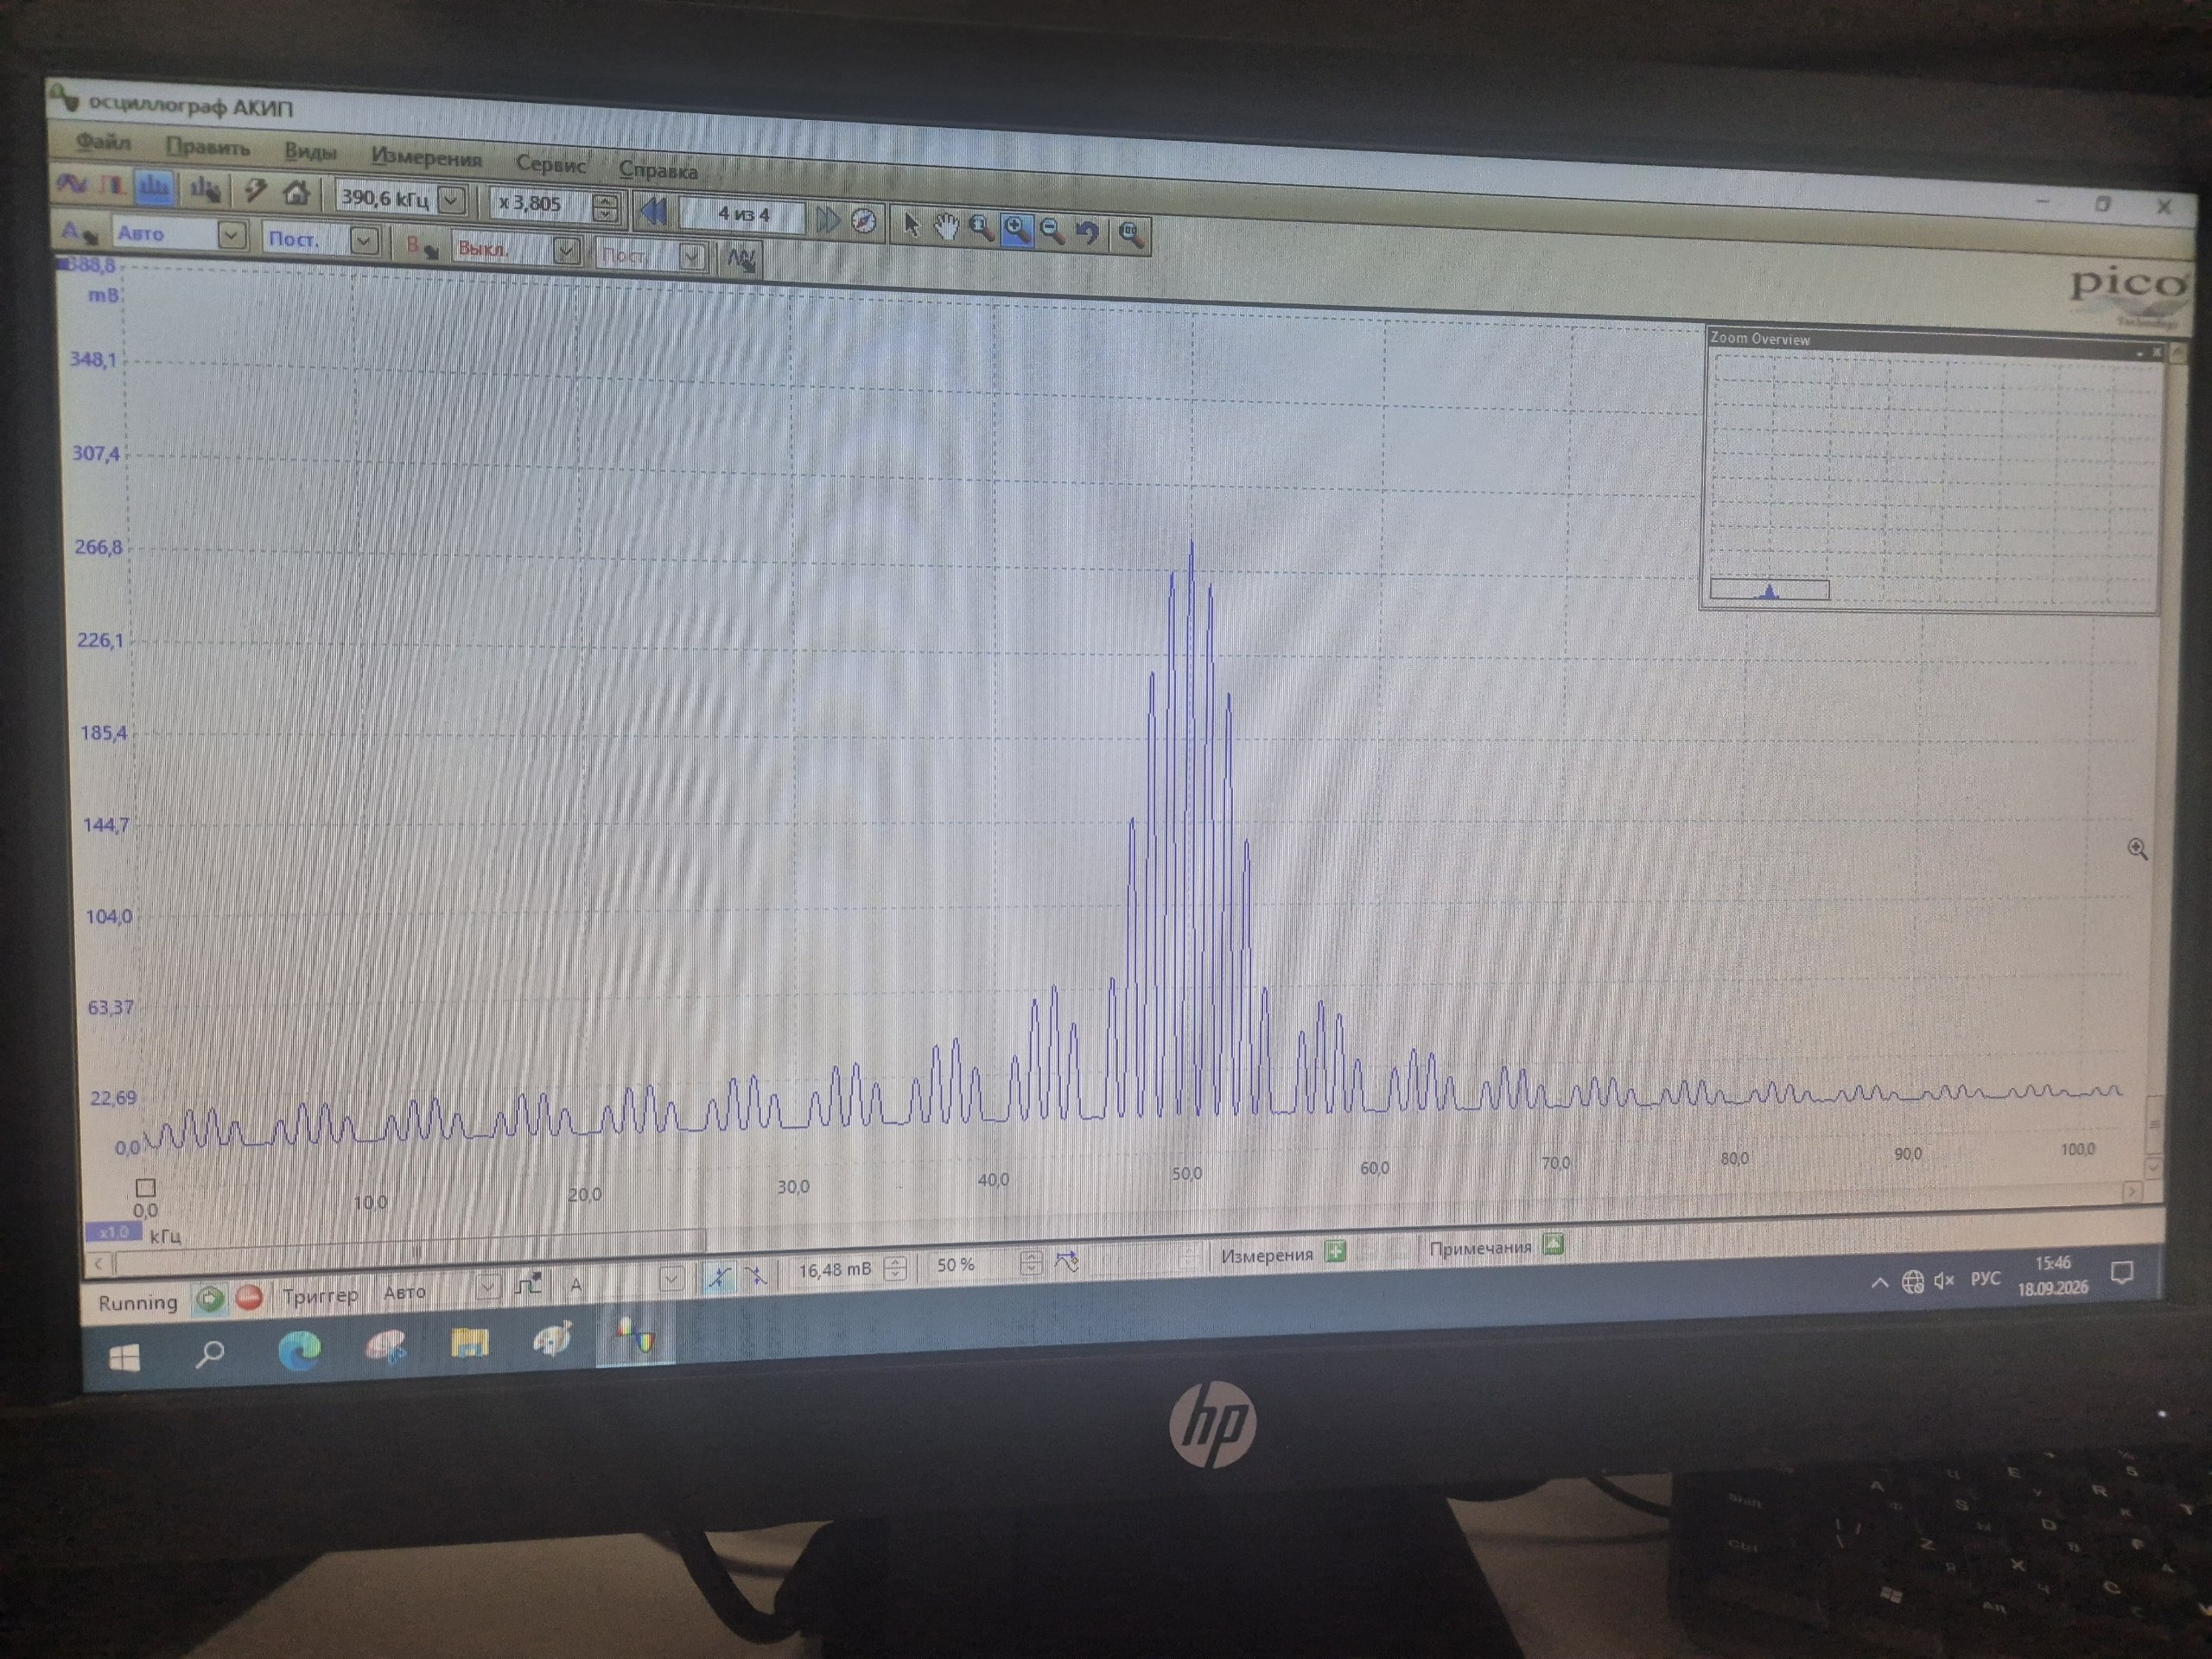
\includegraphics[width=\textwidth]{images/B_N10.jpg}
        \caption{$N=10$}
    \end{subfigure}

    \vspace{0.5cm}

    \begin{subfigure}{0.48\textwidth}
        \centering
        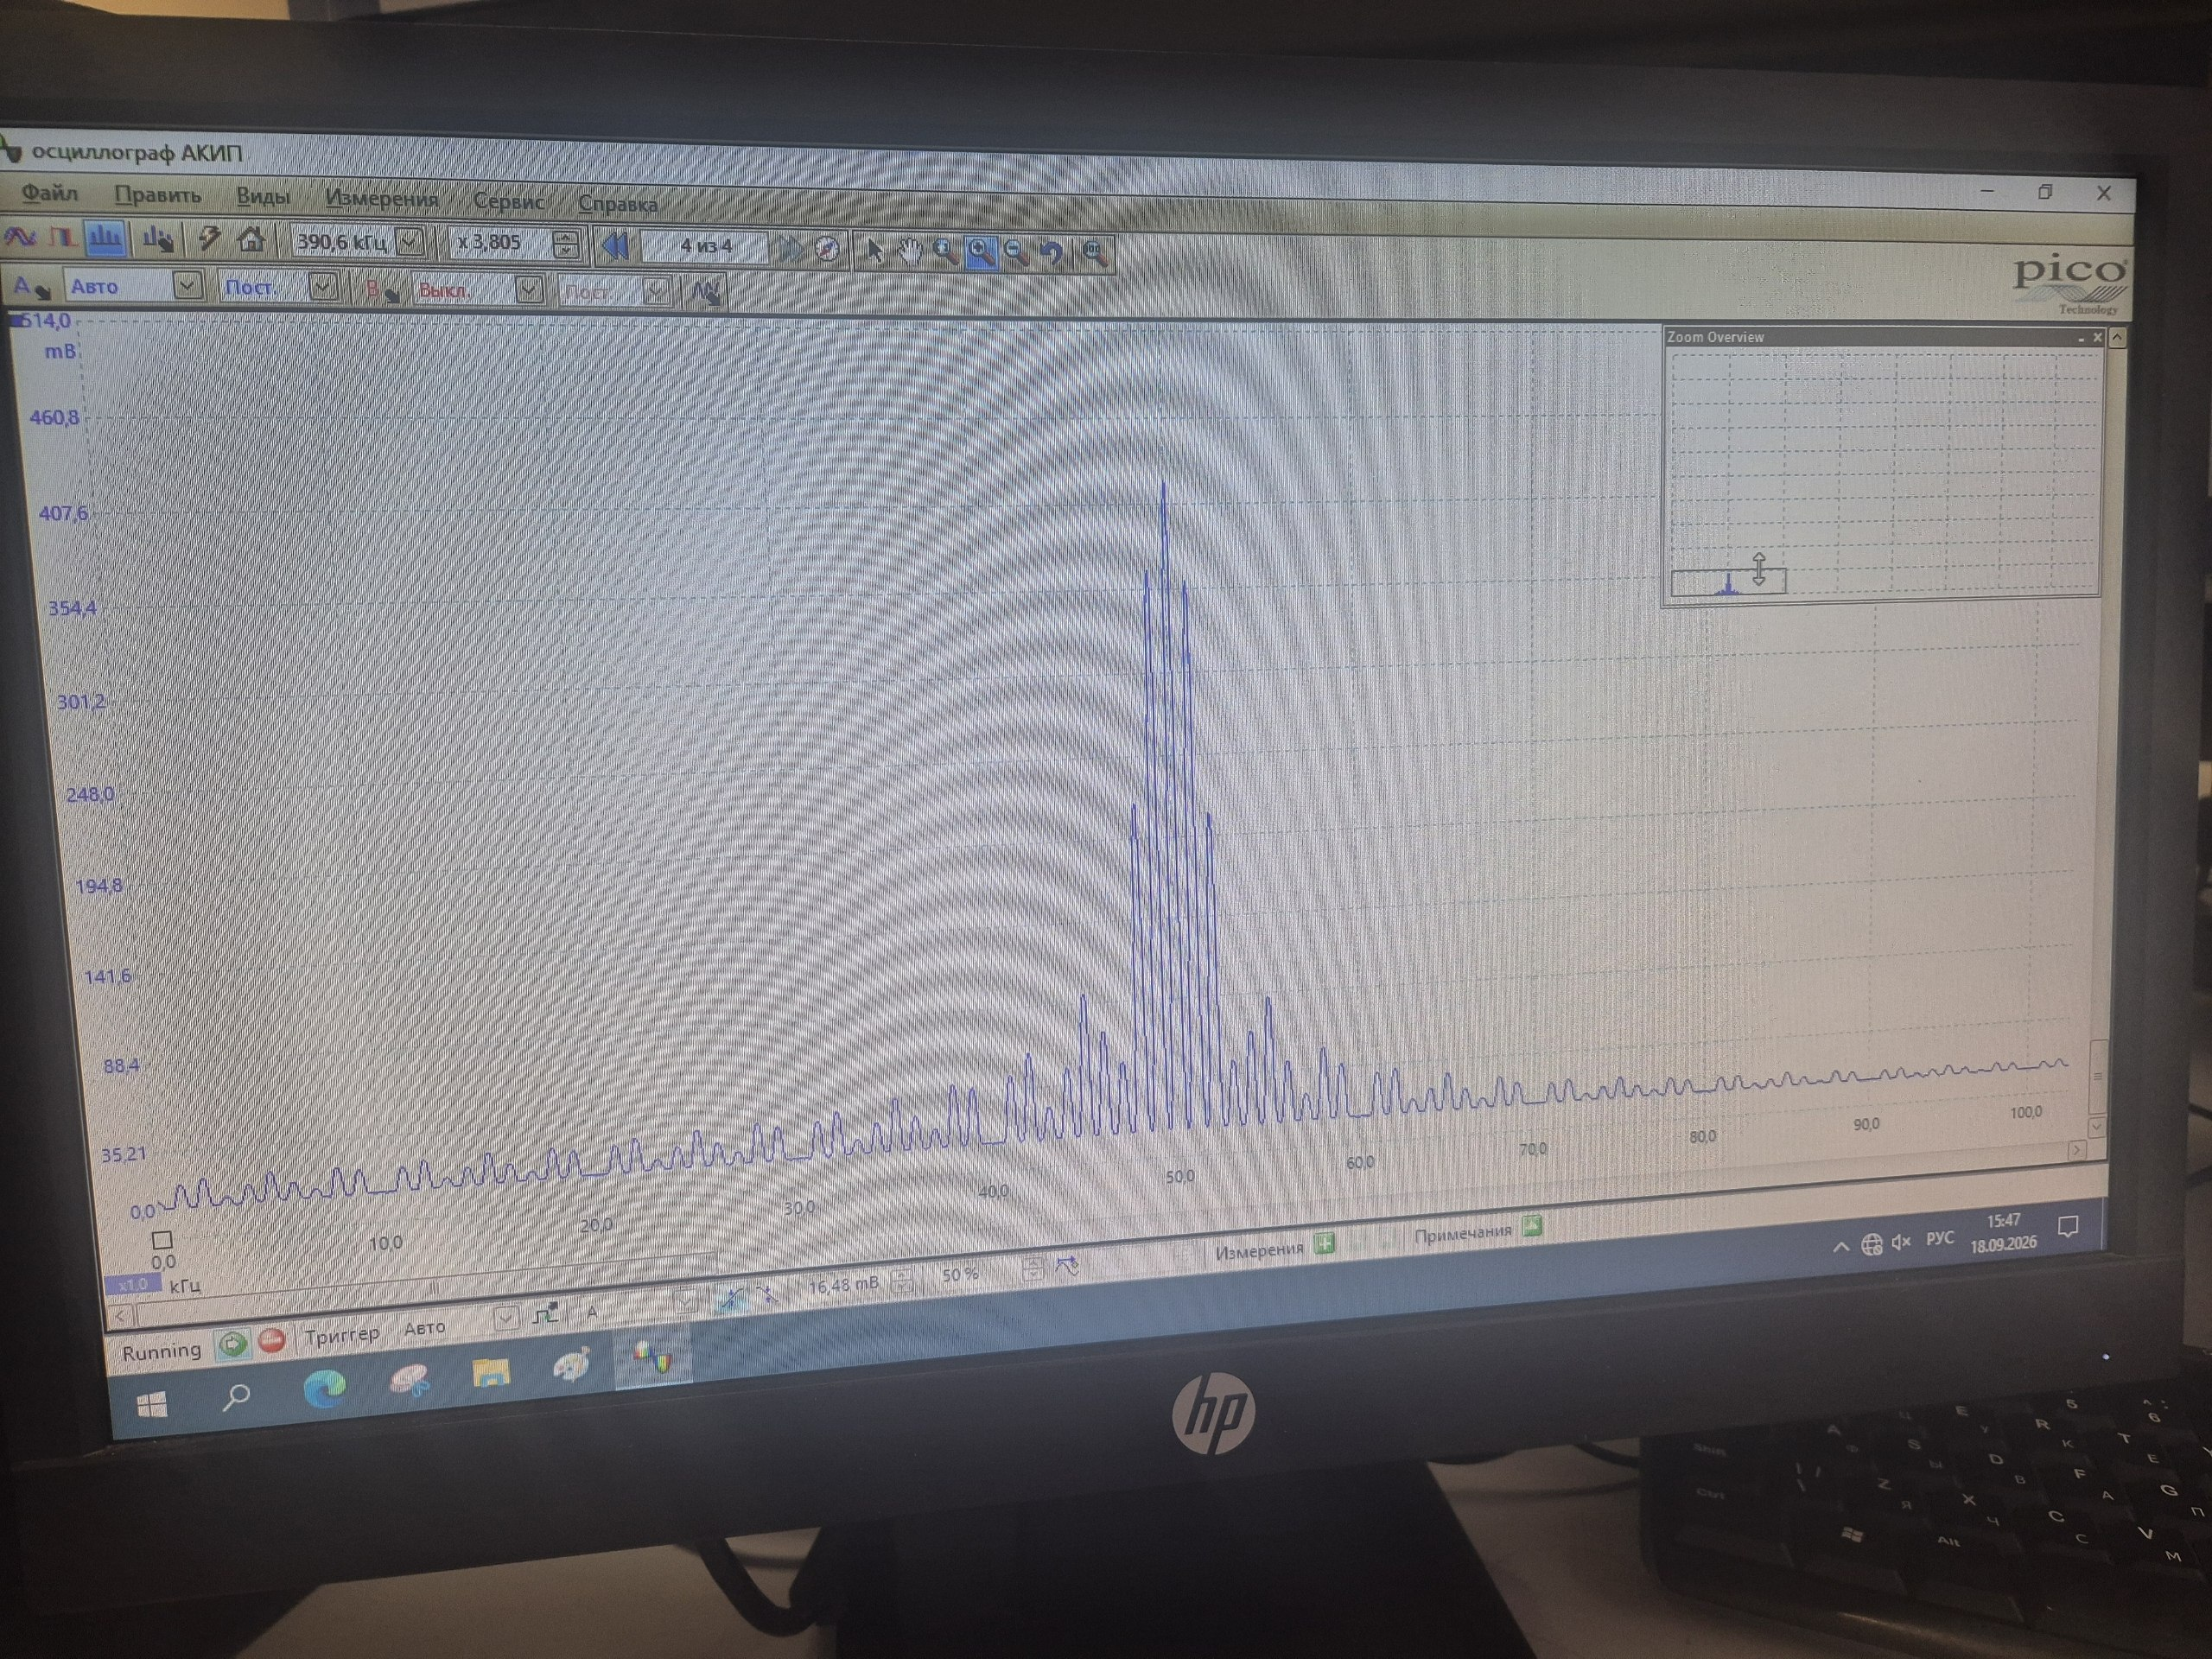
\includegraphics[width=\textwidth]{images/B_N15.jpg}
        \caption{$N=15$}
    \end{subfigure}
    \hfill
    \begin{subfigure}{0.48\textwidth}
        \centering
        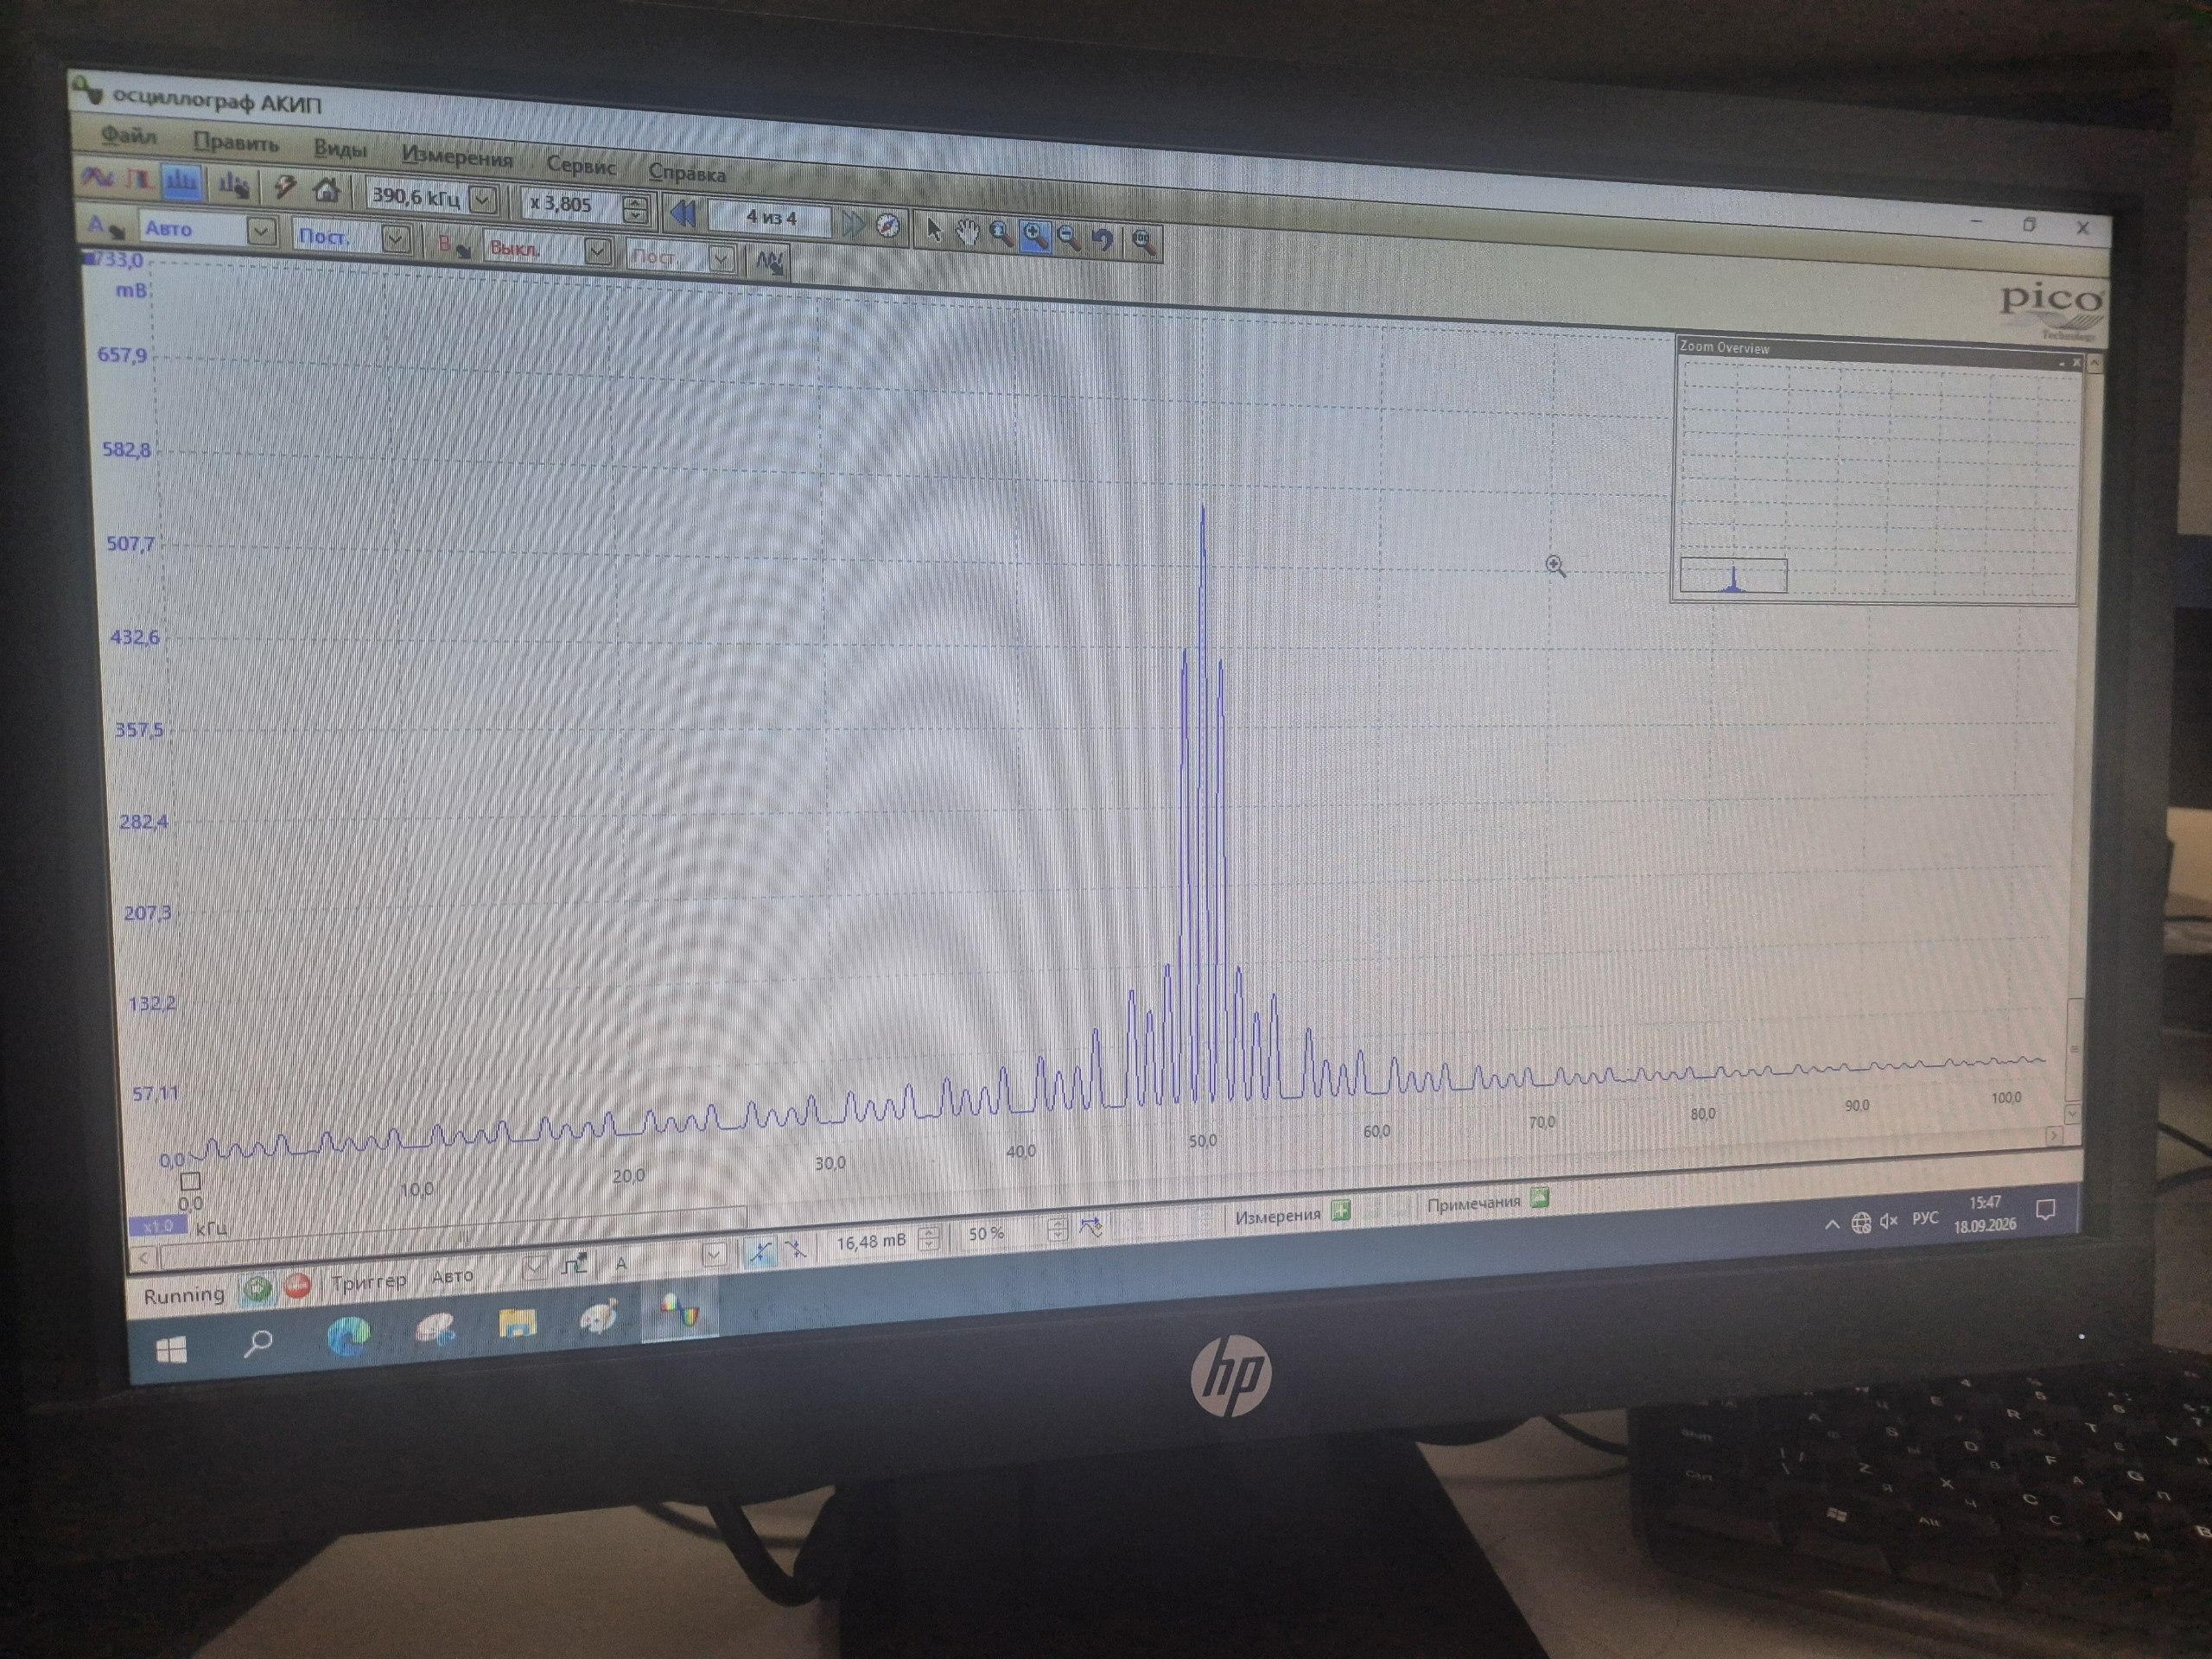
\includegraphics[width=\textwidth]{images/B_N20.jpg}
        \caption{$N=20$}
    \end{subfigure}

    \caption{Спектры периодической последовательности цугов при
    различных значениях числа периодов $N$.}
\end{figure}

\newpage

\subsubsection*{Изменение периода повторения цугов}

Затем исследовалось влияние периода повторения цугов $T$.
Период изменялся от $1$ до $4$ мс.

\begin{figure}[H]
    \centering

    \begin{subfigure}{0.48\textwidth}
        \centering
        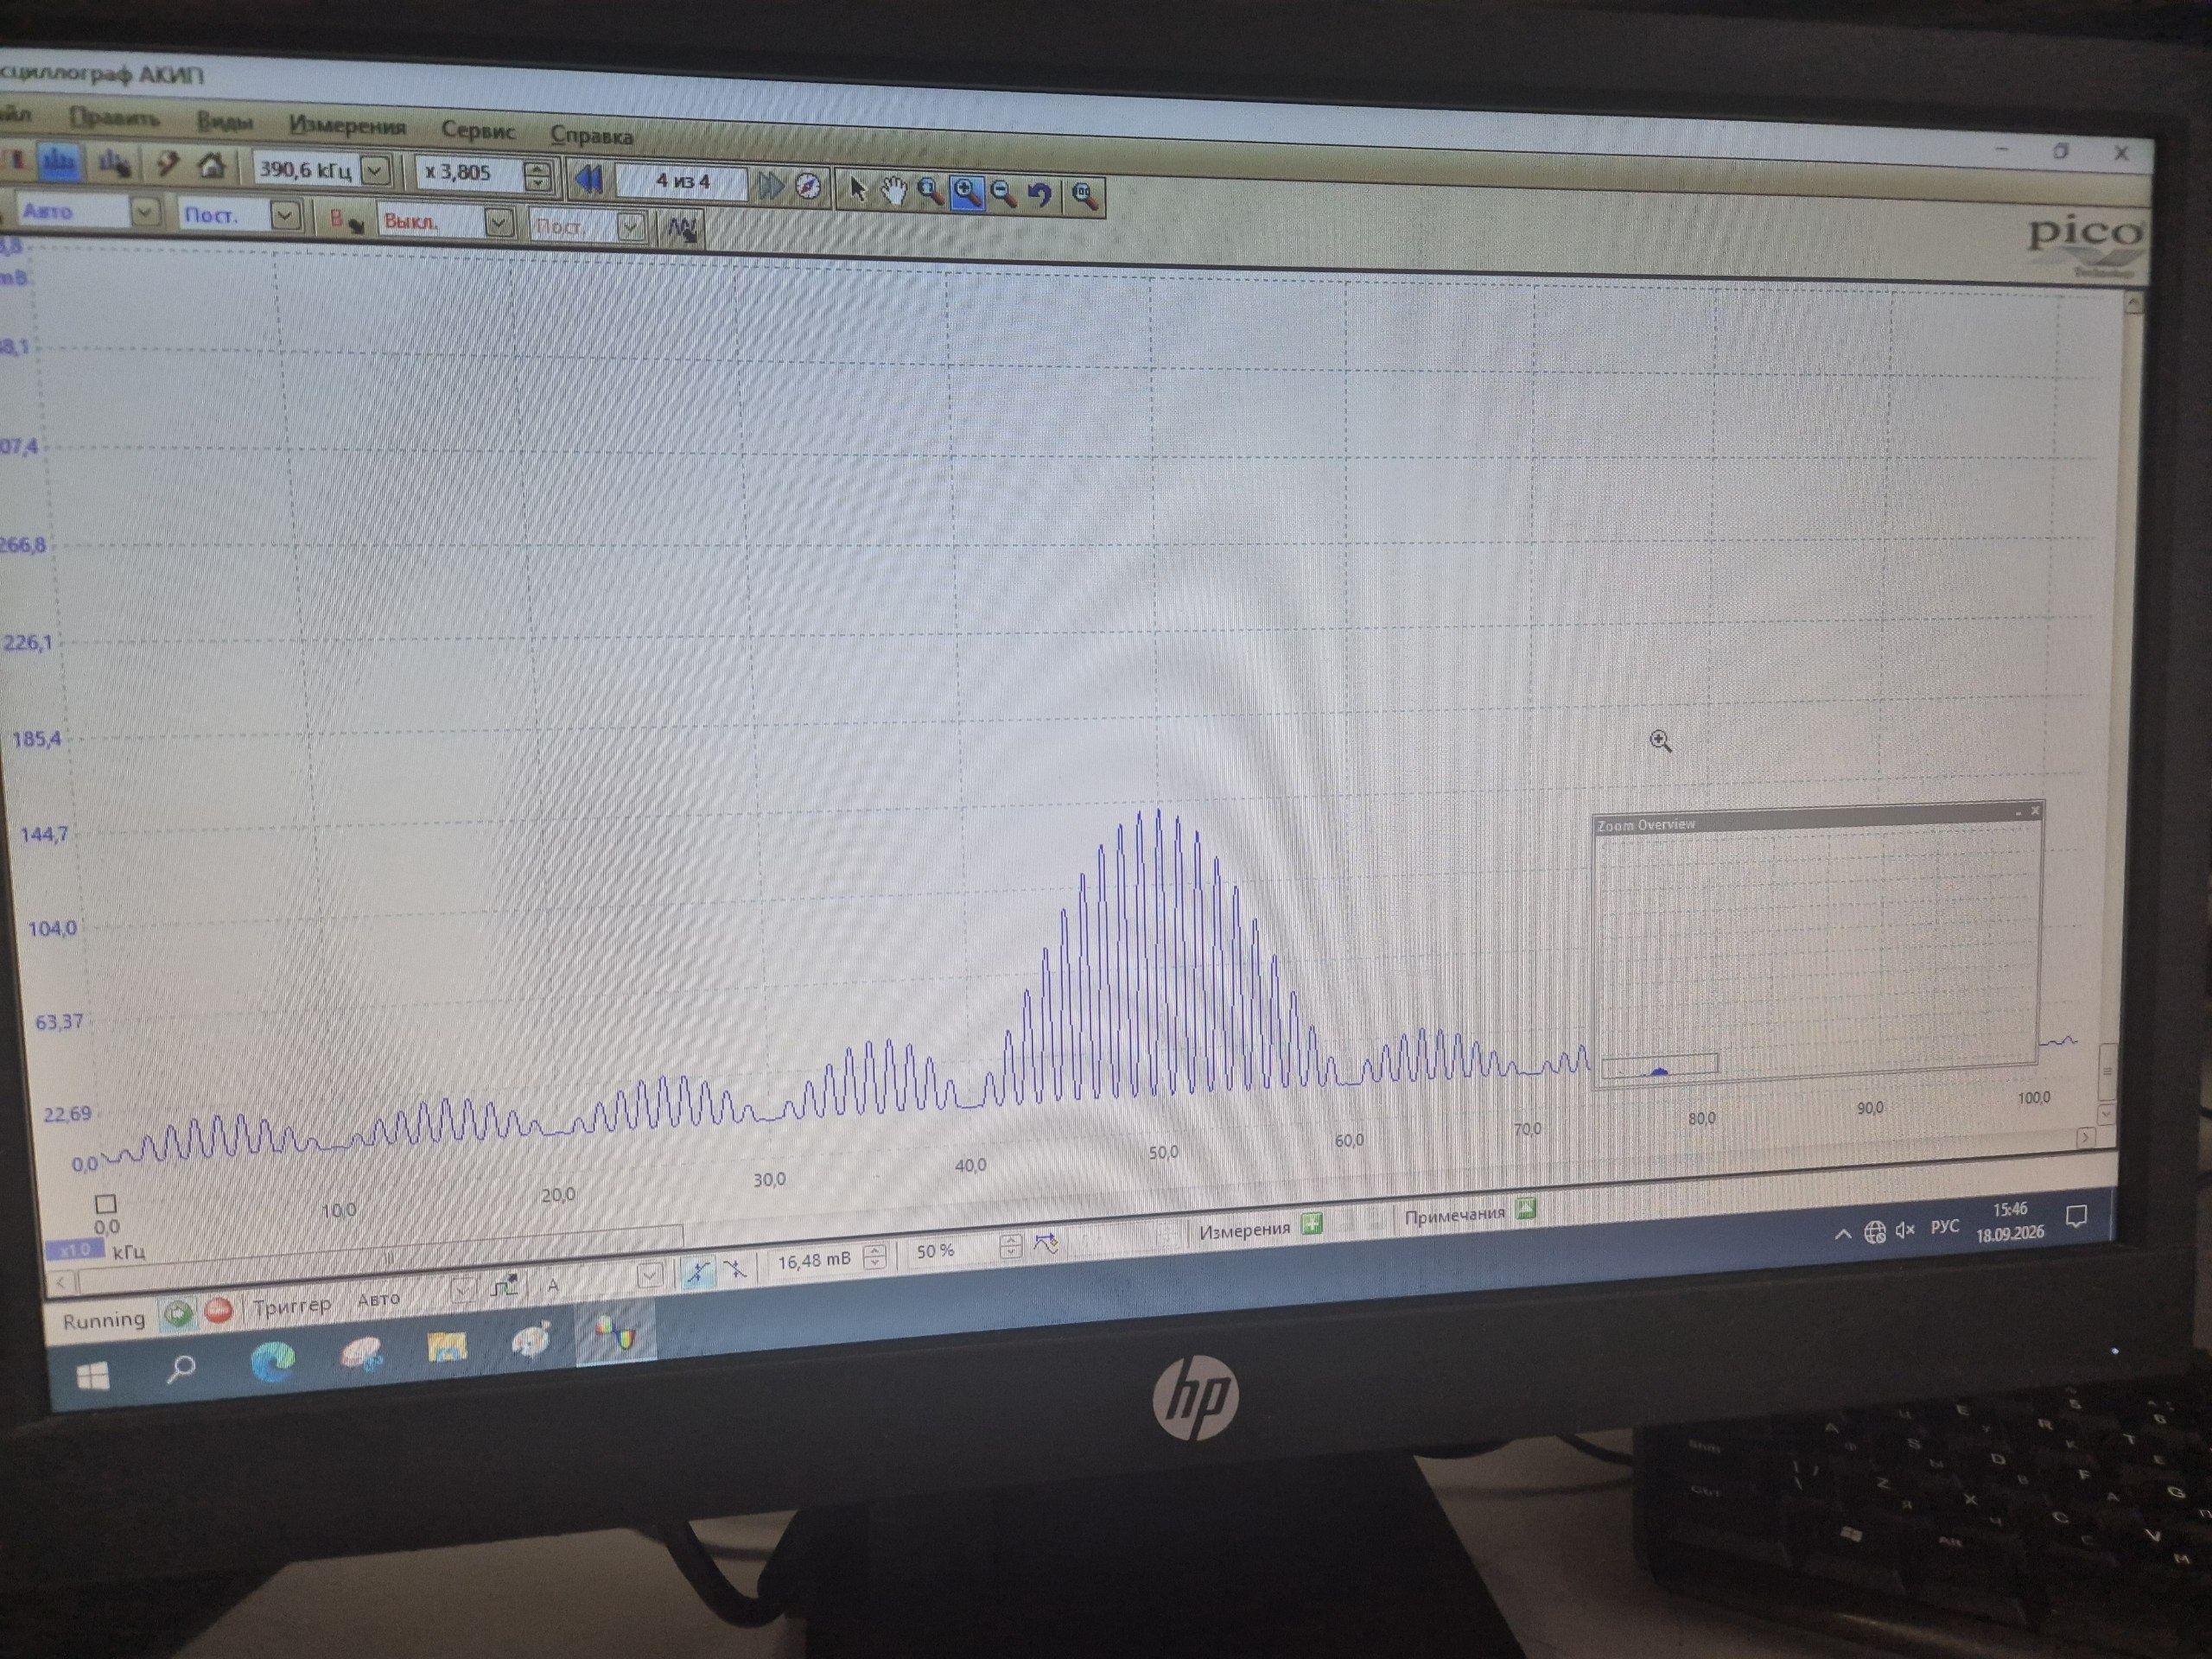
\includegraphics[width=\textwidth]{images/B_T1.jpg}
        \caption{$T=1$ мс}
    \end{subfigure}
    \hfill
    \begin{subfigure}{0.48\textwidth}
        \centering
        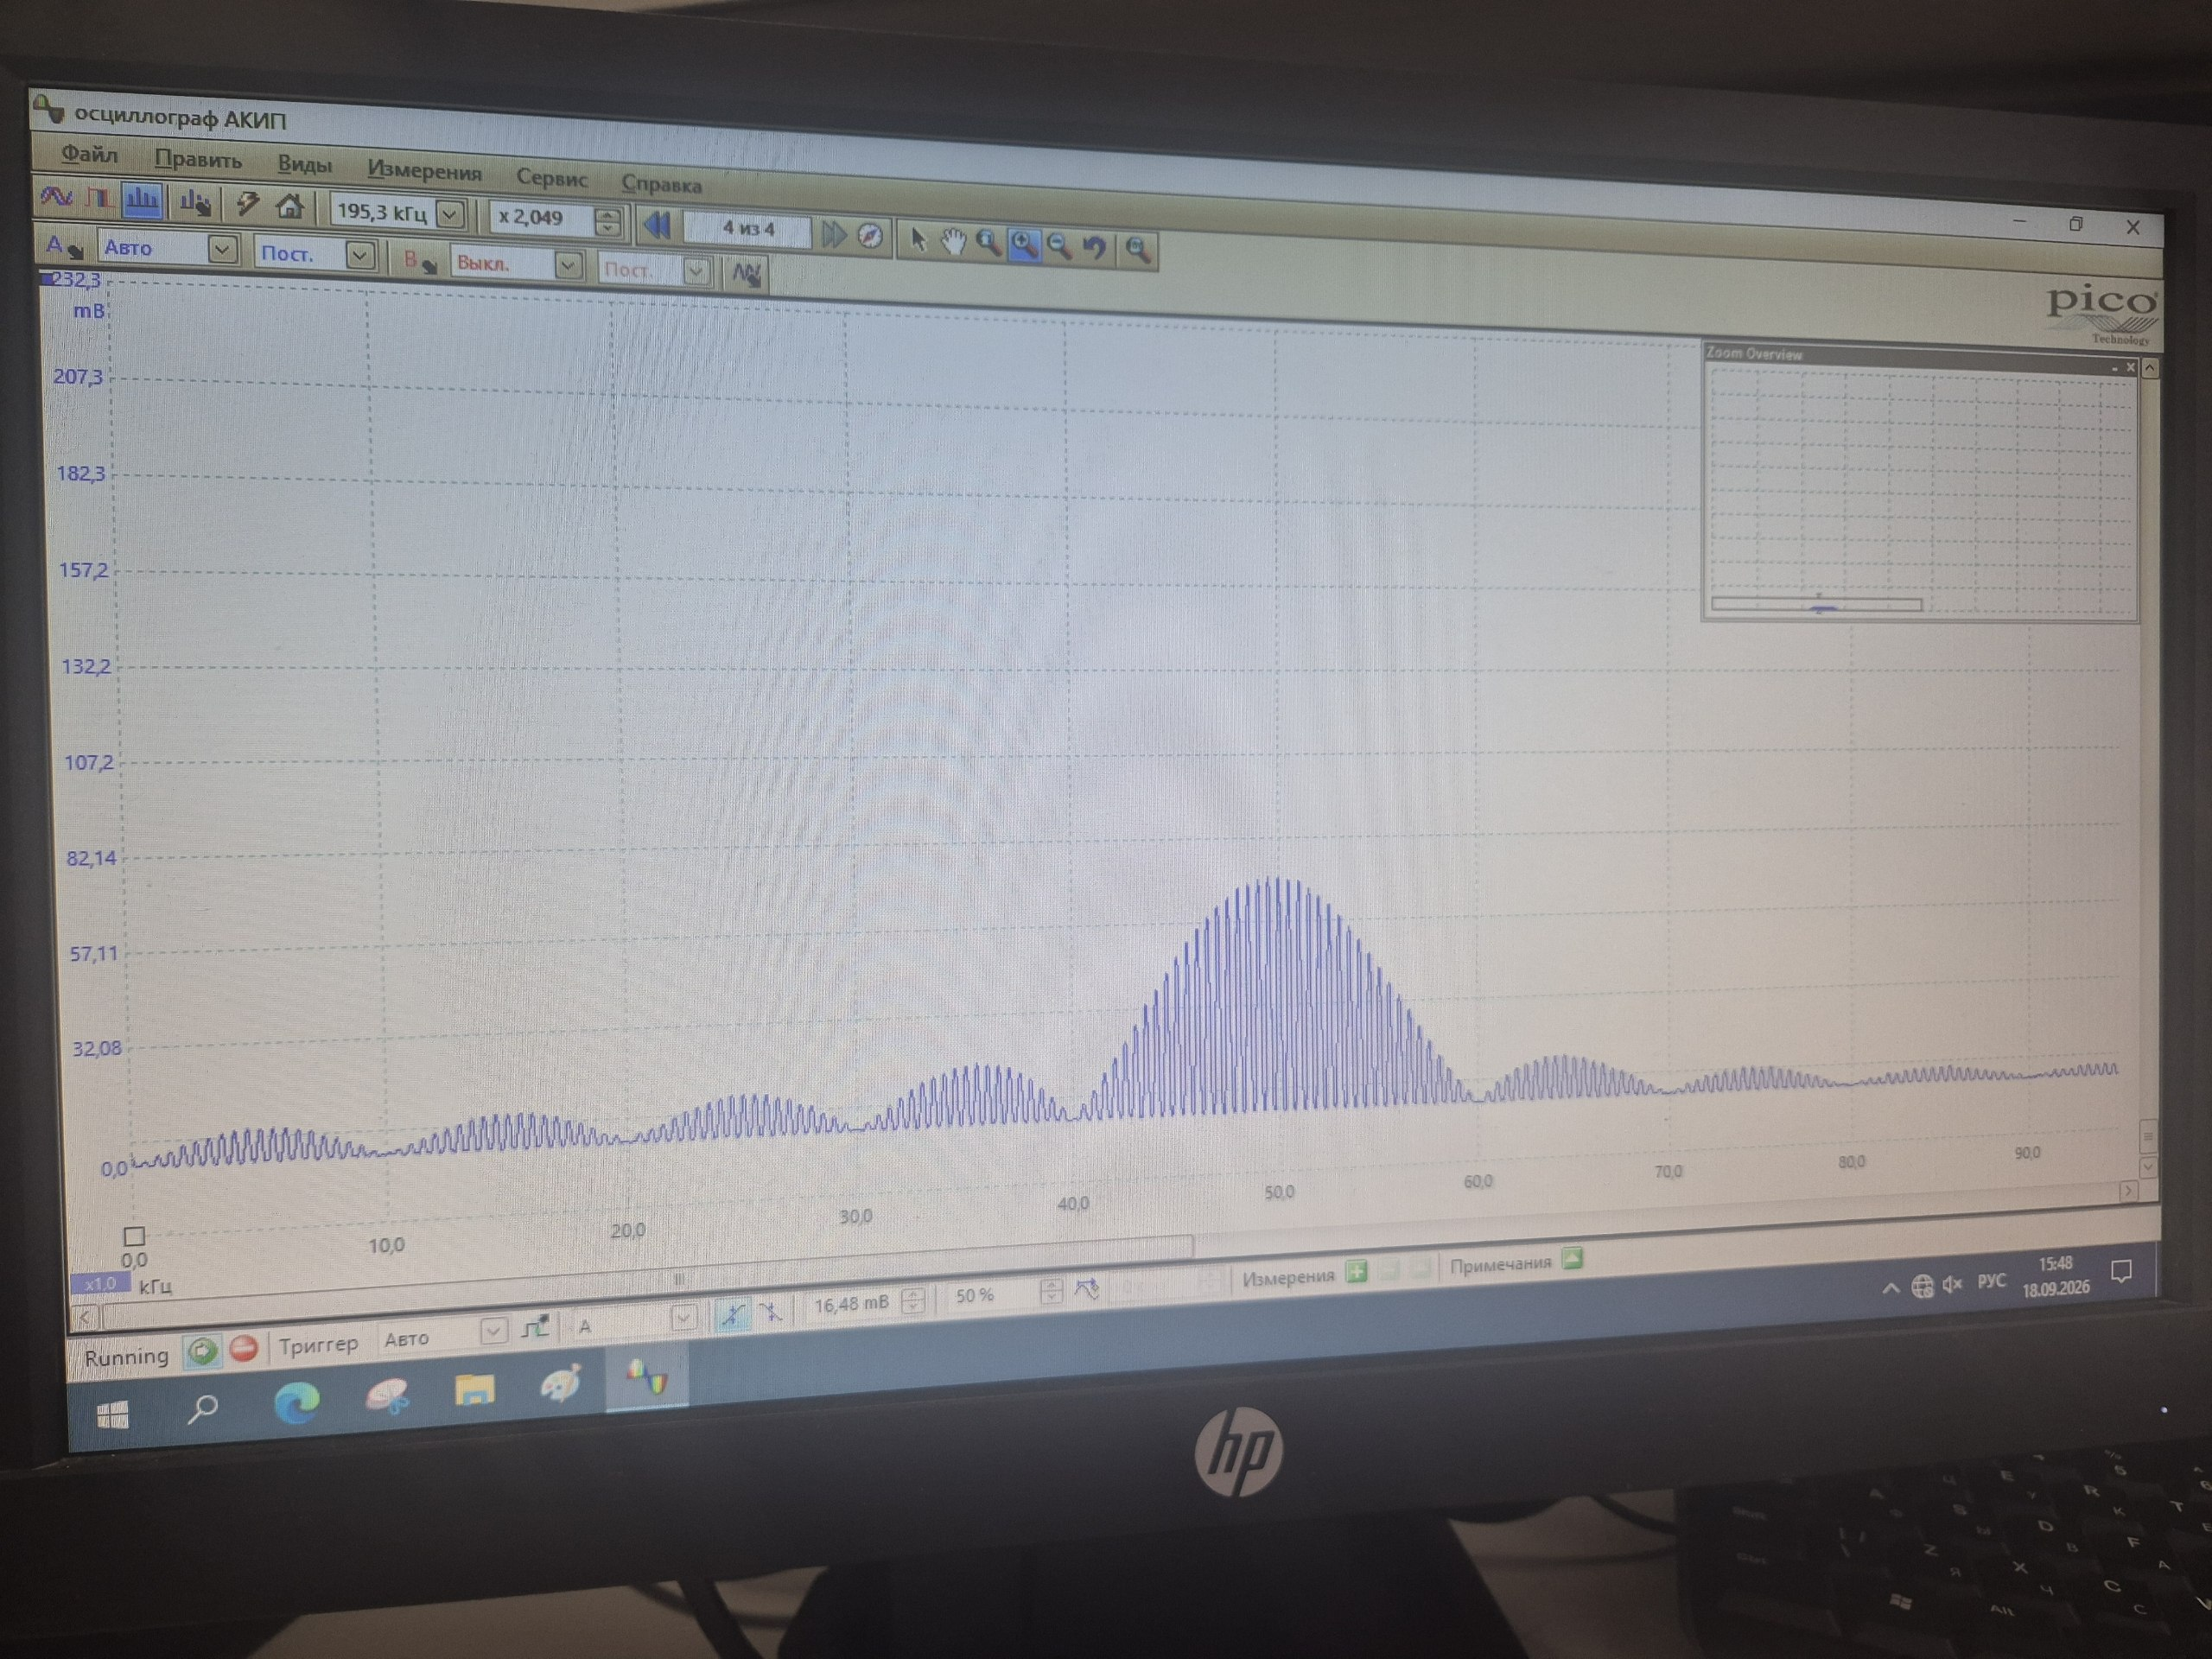
\includegraphics[width=\textwidth]{images/B_T2.jpg}
        \caption{$T=2$ мс}
    \end{subfigure}

    \vspace{0.5cm}

    \begin{subfigure}{0.48\textwidth}
        \centering
        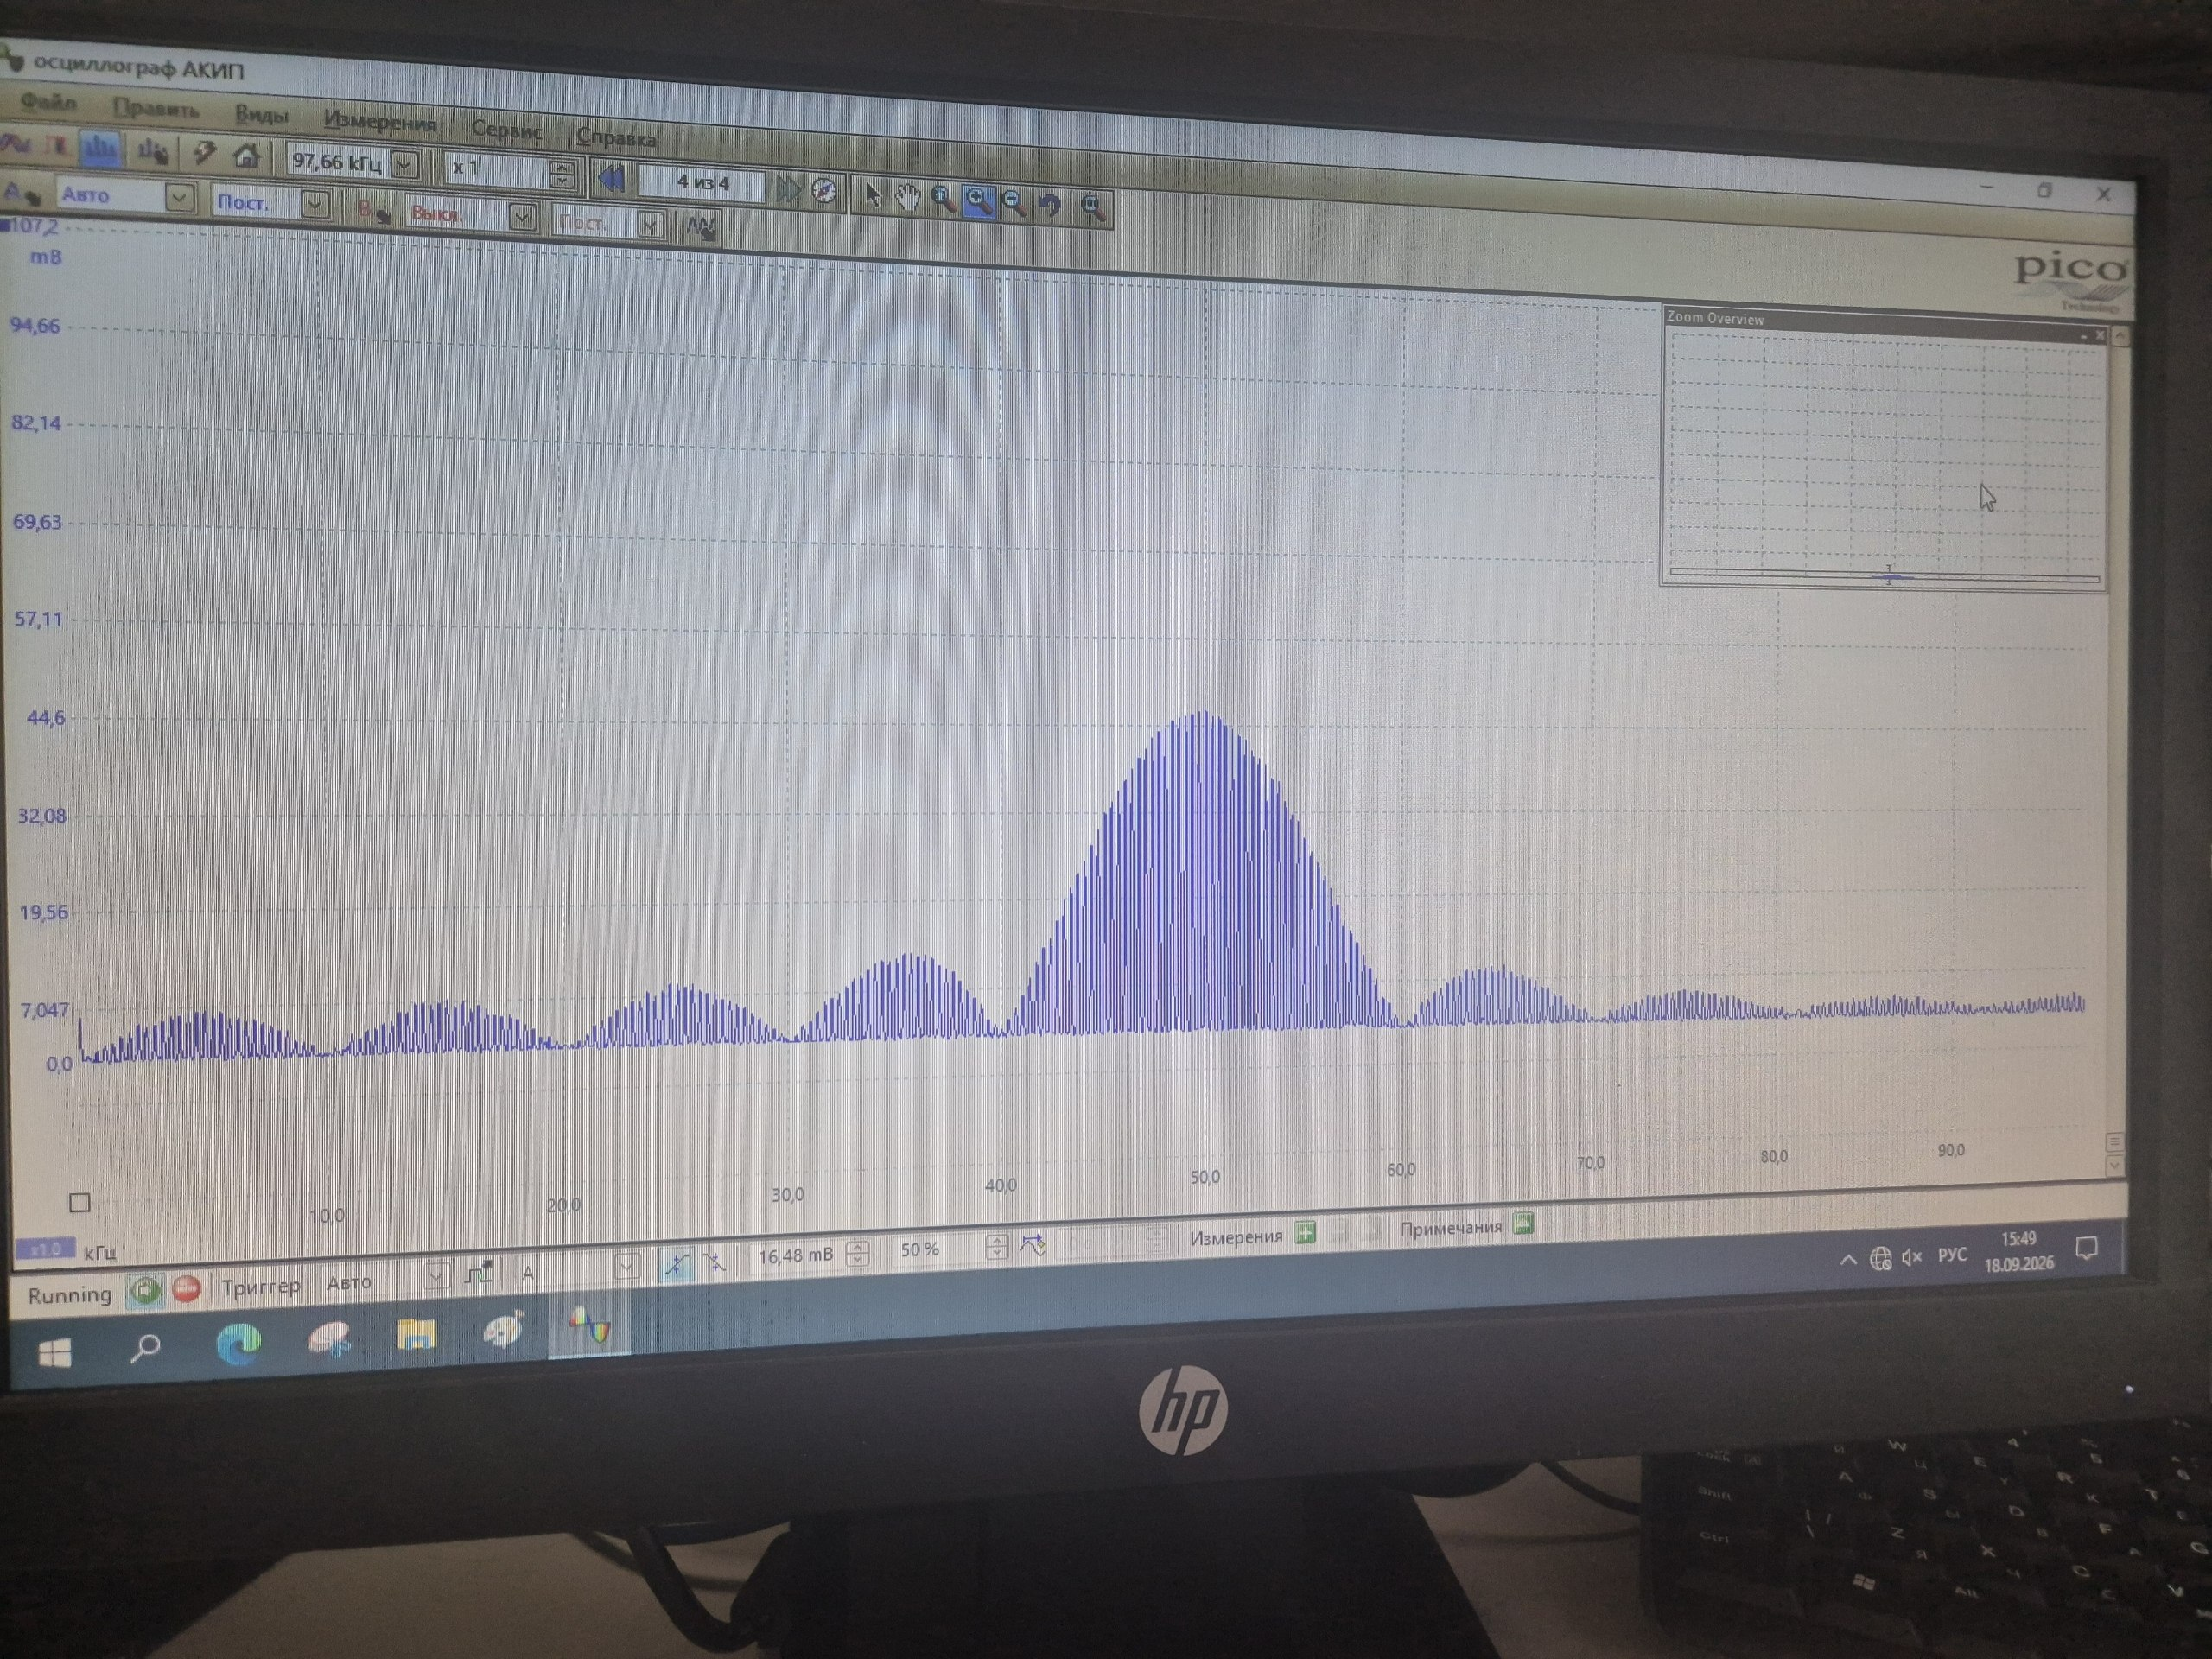
\includegraphics[width=\textwidth]{images/B_T3.jpg}
        \caption{$T=3$ мс}
    \end{subfigure}
    \hfill
    \begin{subfigure}{0.48\textwidth}
        \centering
        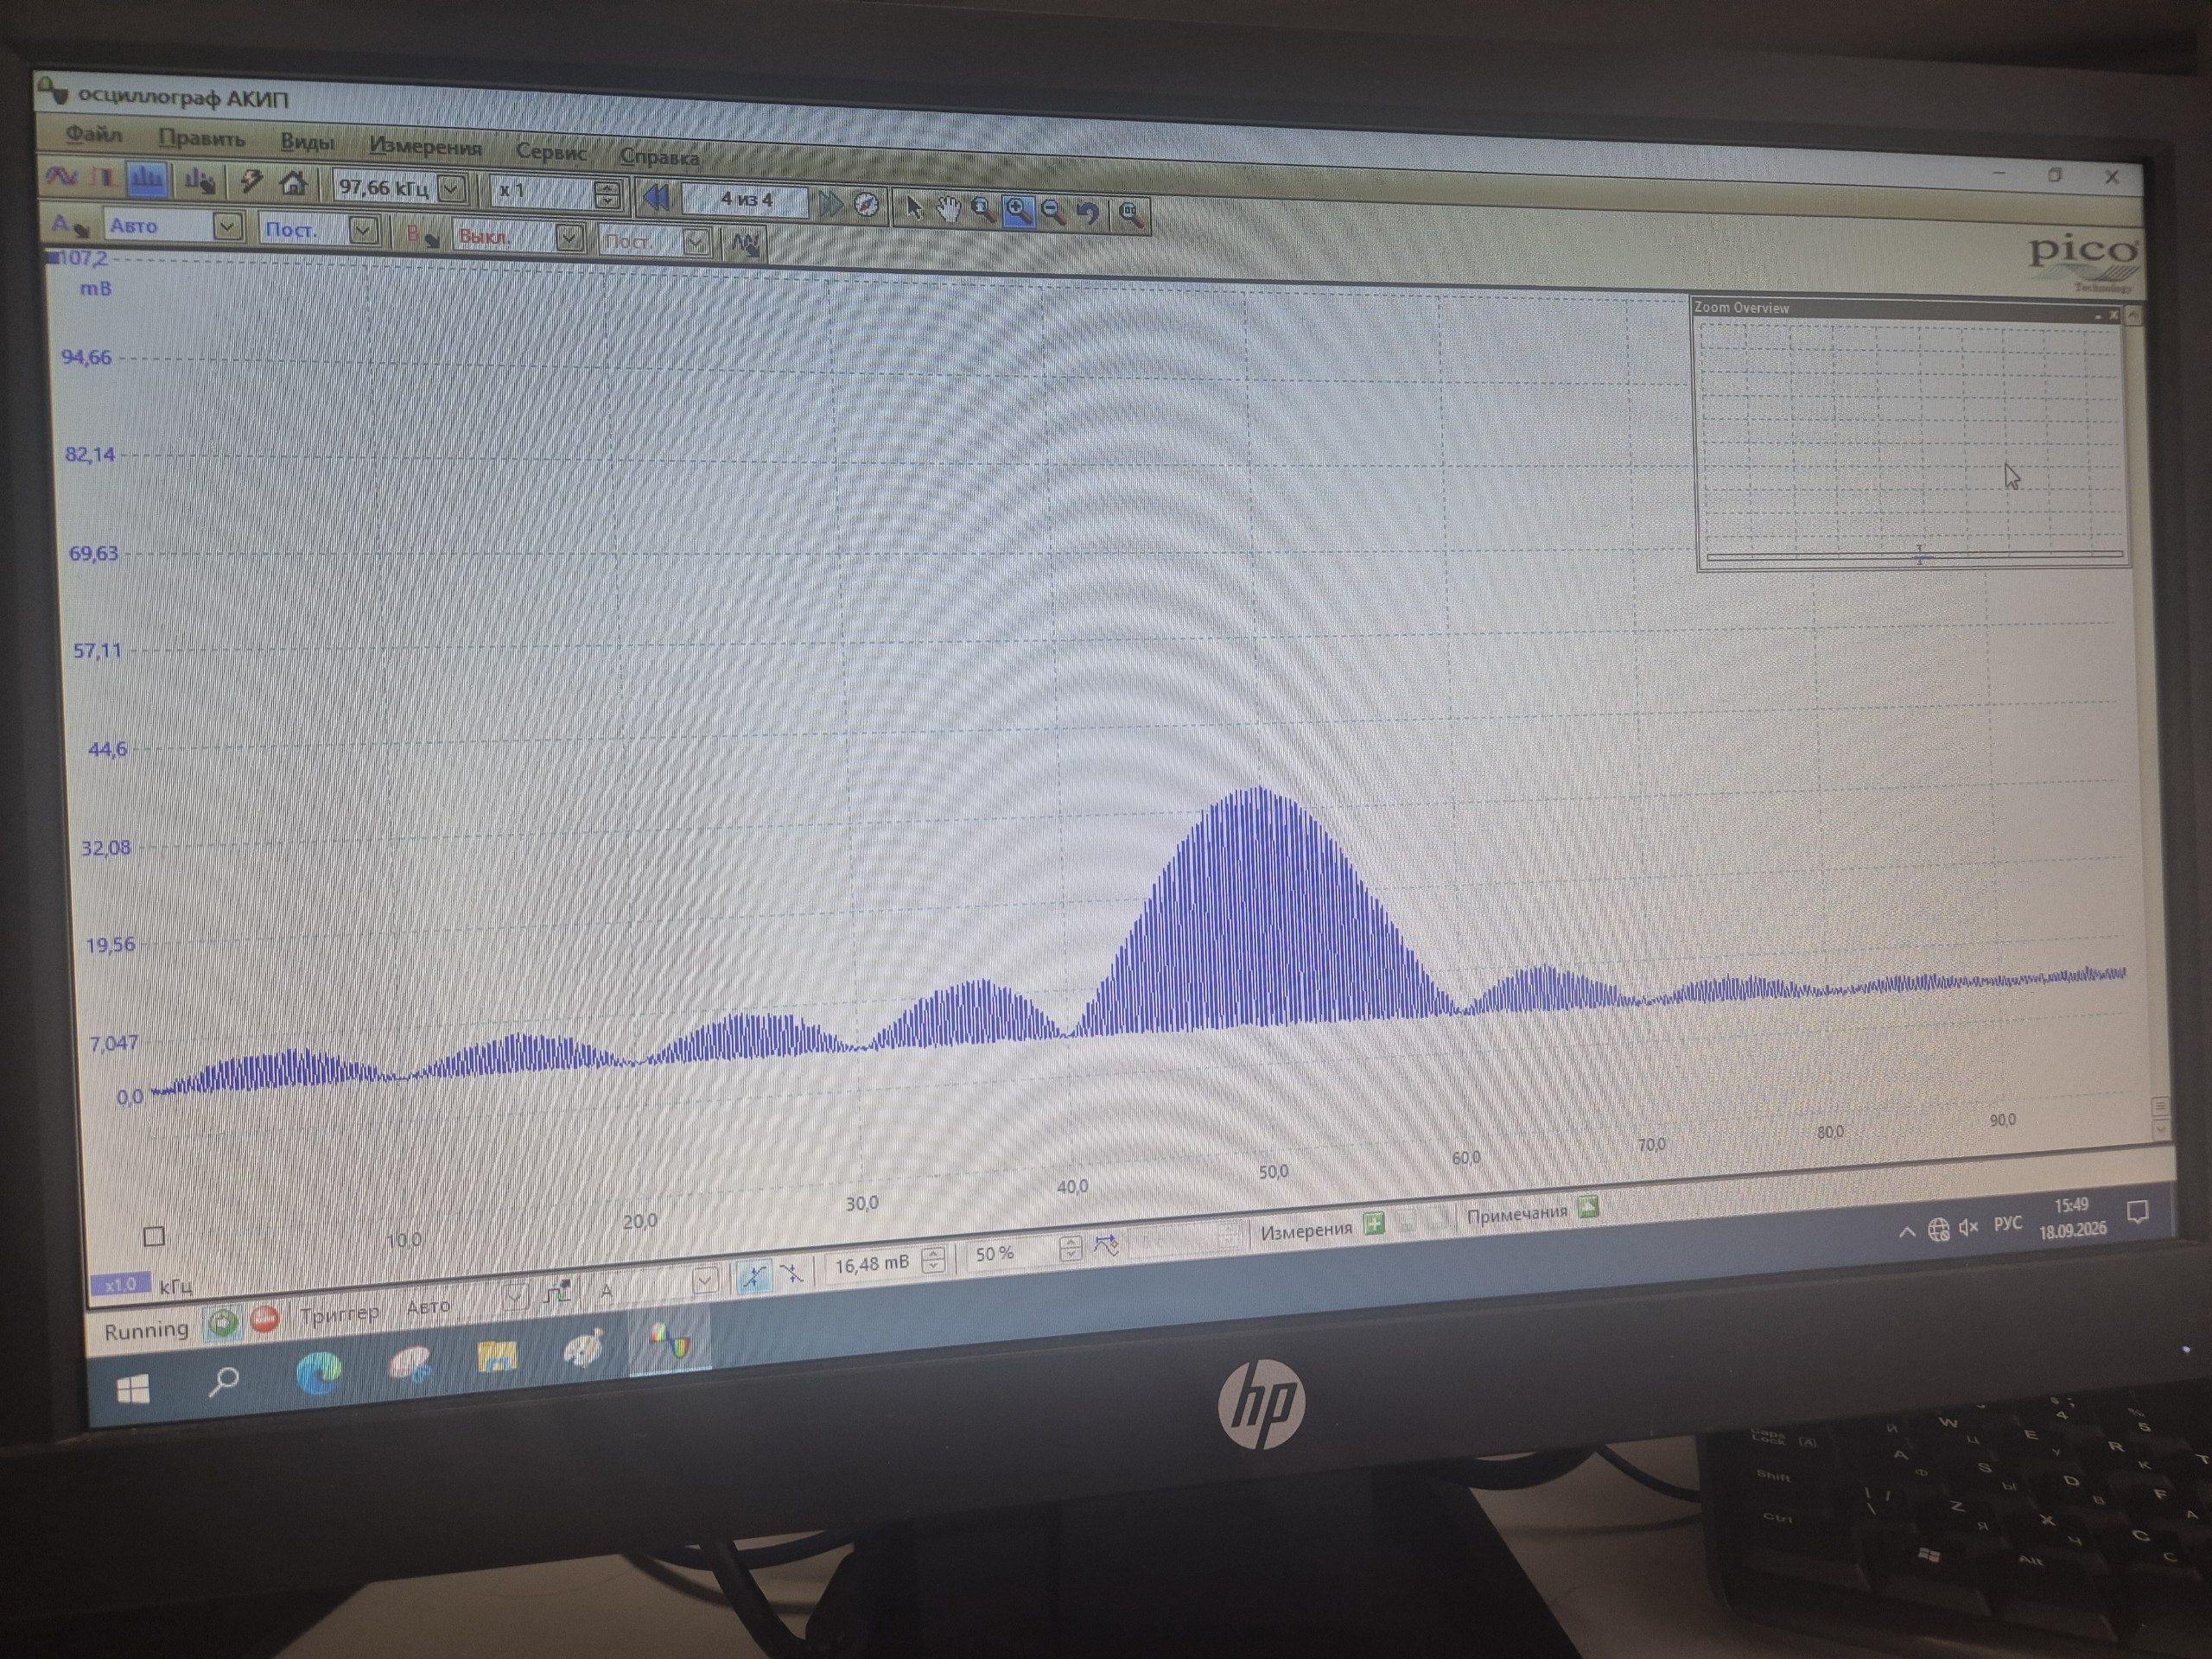
\includegraphics[width=\textwidth]{images/B_T4.jpg}
        \caption{$T=4$ мс}
    \end{subfigure}

    \caption{Спектры периодической последовательности цугов при
    различных значениях периода повторения $T$.}
\end{figure}

\newpage

\subsubsection*{Изменение частоты заполнения}

Наконец, исследовалось влияние частоты заполнения $\nu_0$.
Частота изменялась от $50$ до $200$ кГц.

\begin{figure}[H]
    \centering

    \begin{subfigure}{0.40\textwidth}
        \centering
        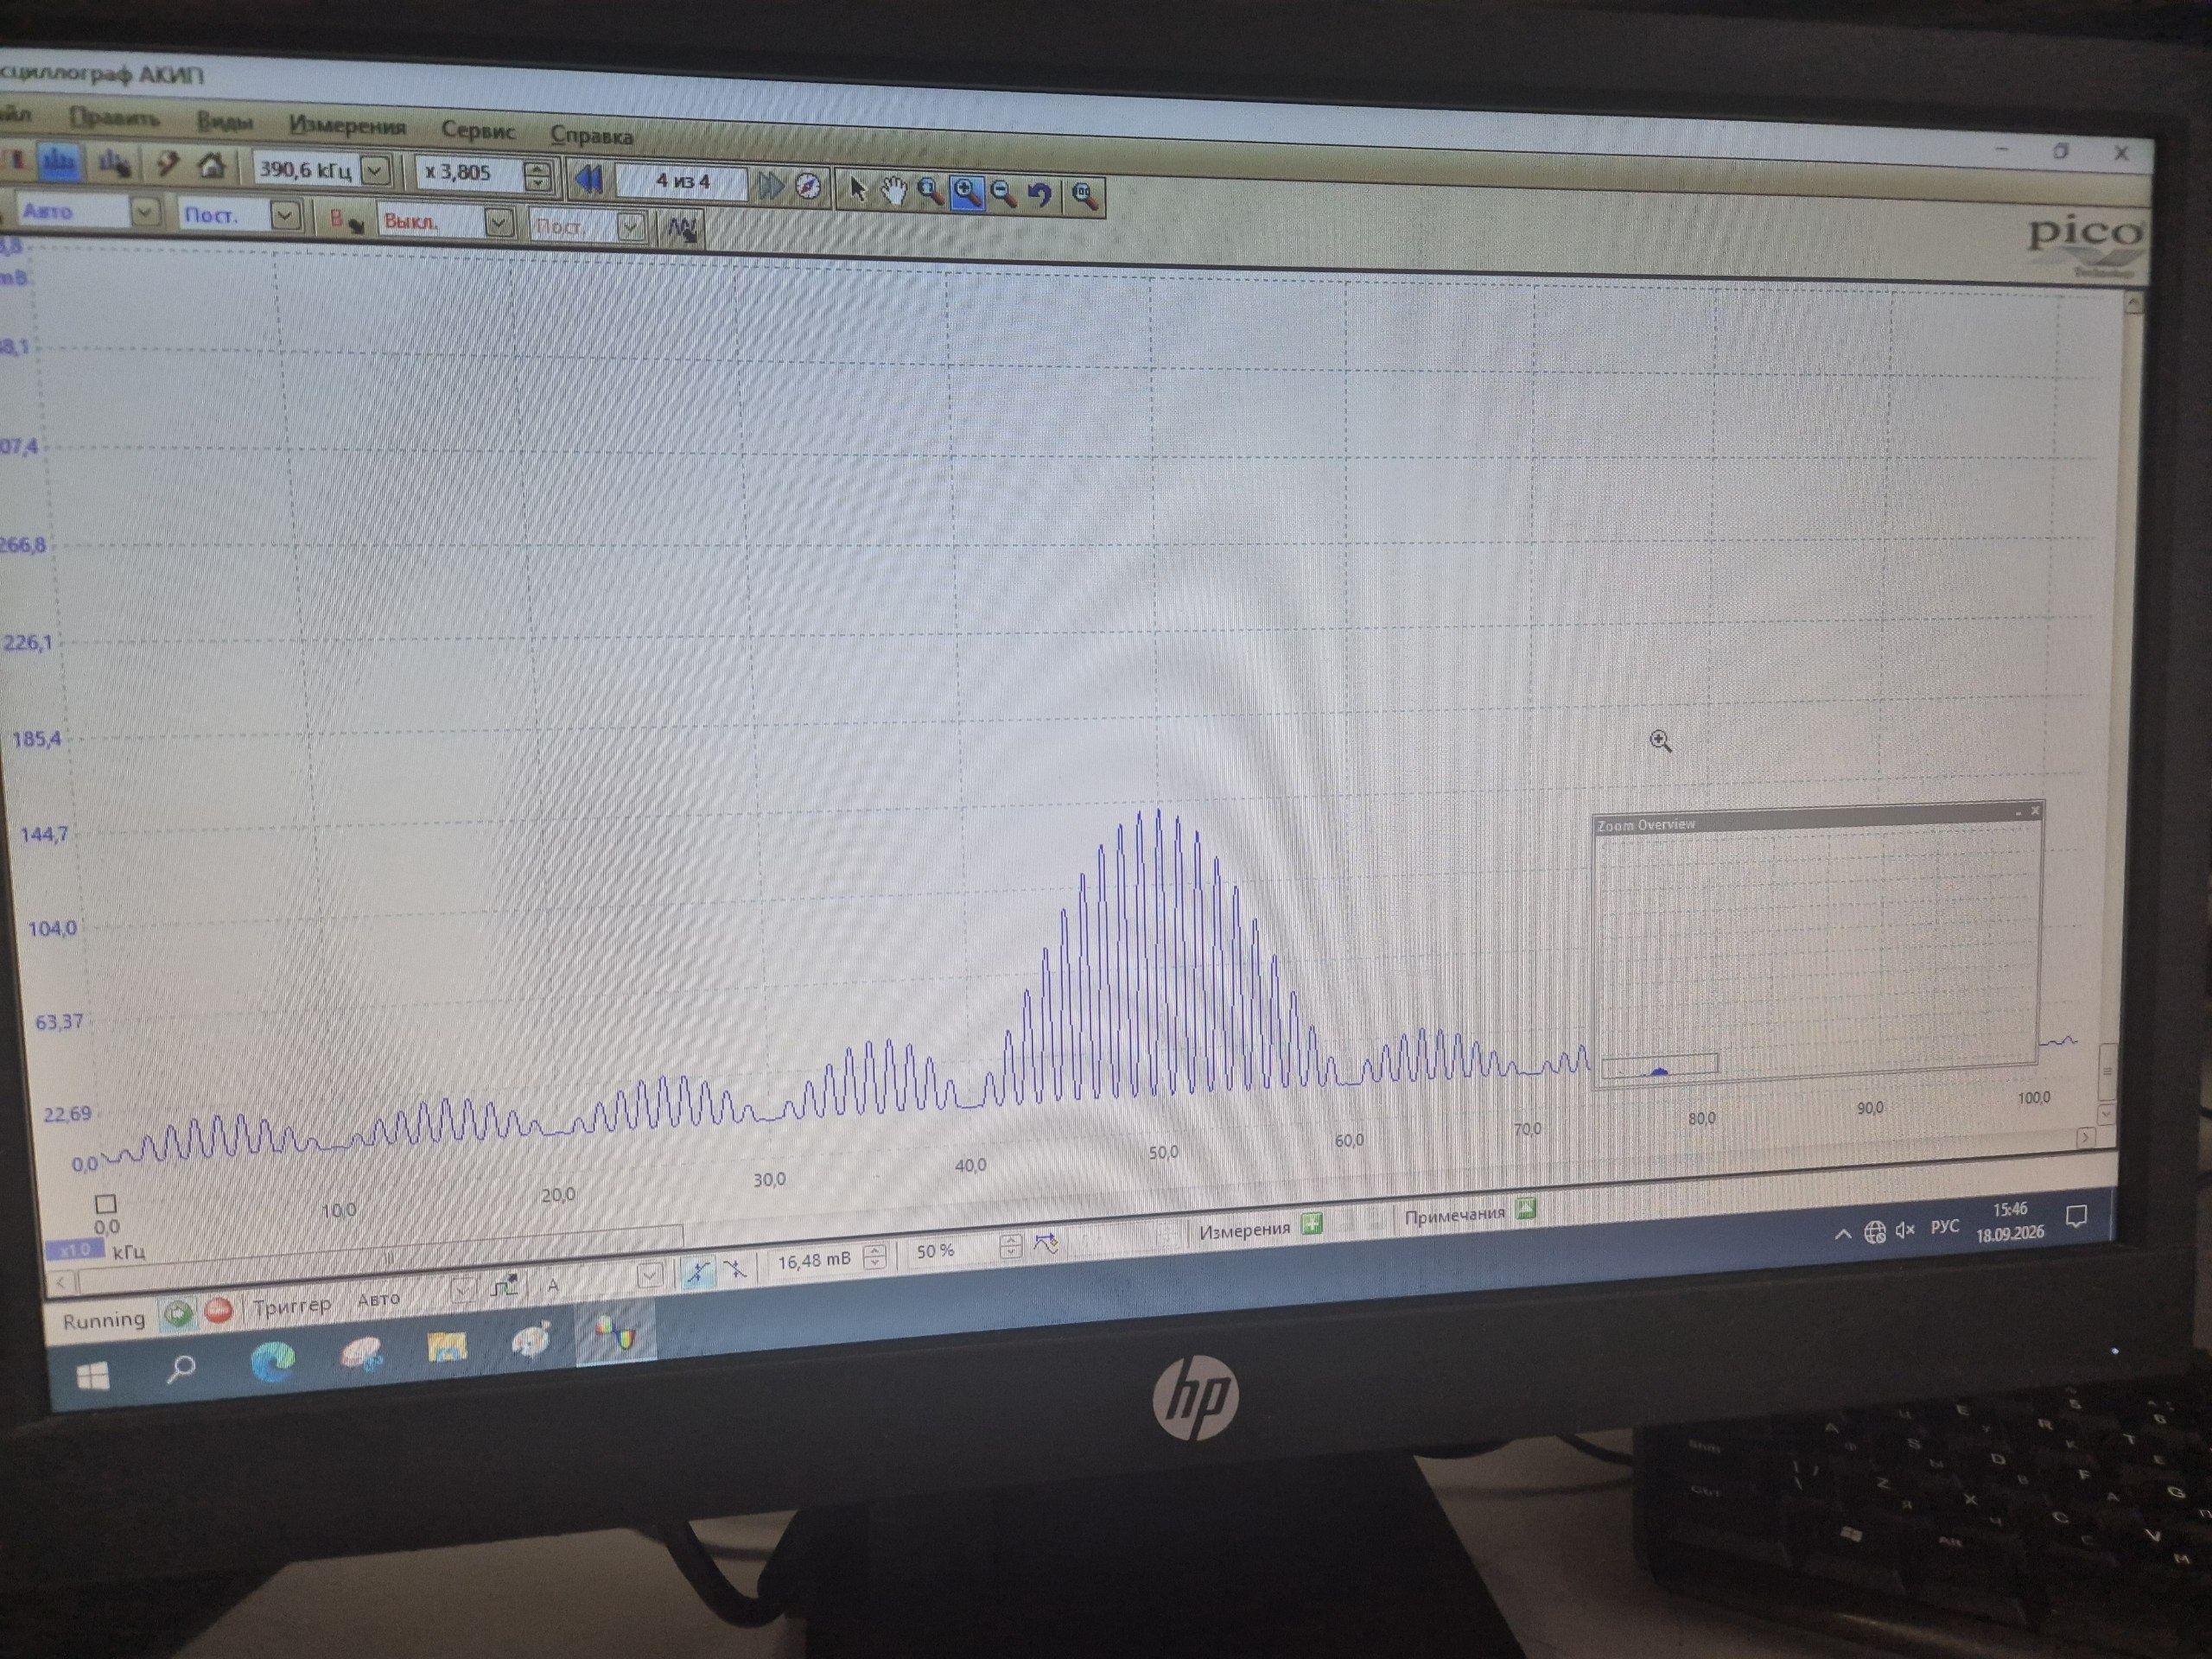
\includegraphics[width=\textwidth]{images/B_nu50.jpg}
        \caption{$\nu_0=50$ кГц}
    \end{subfigure}
    \hfill
    \begin{subfigure}{0.40\textwidth}
        \centering
        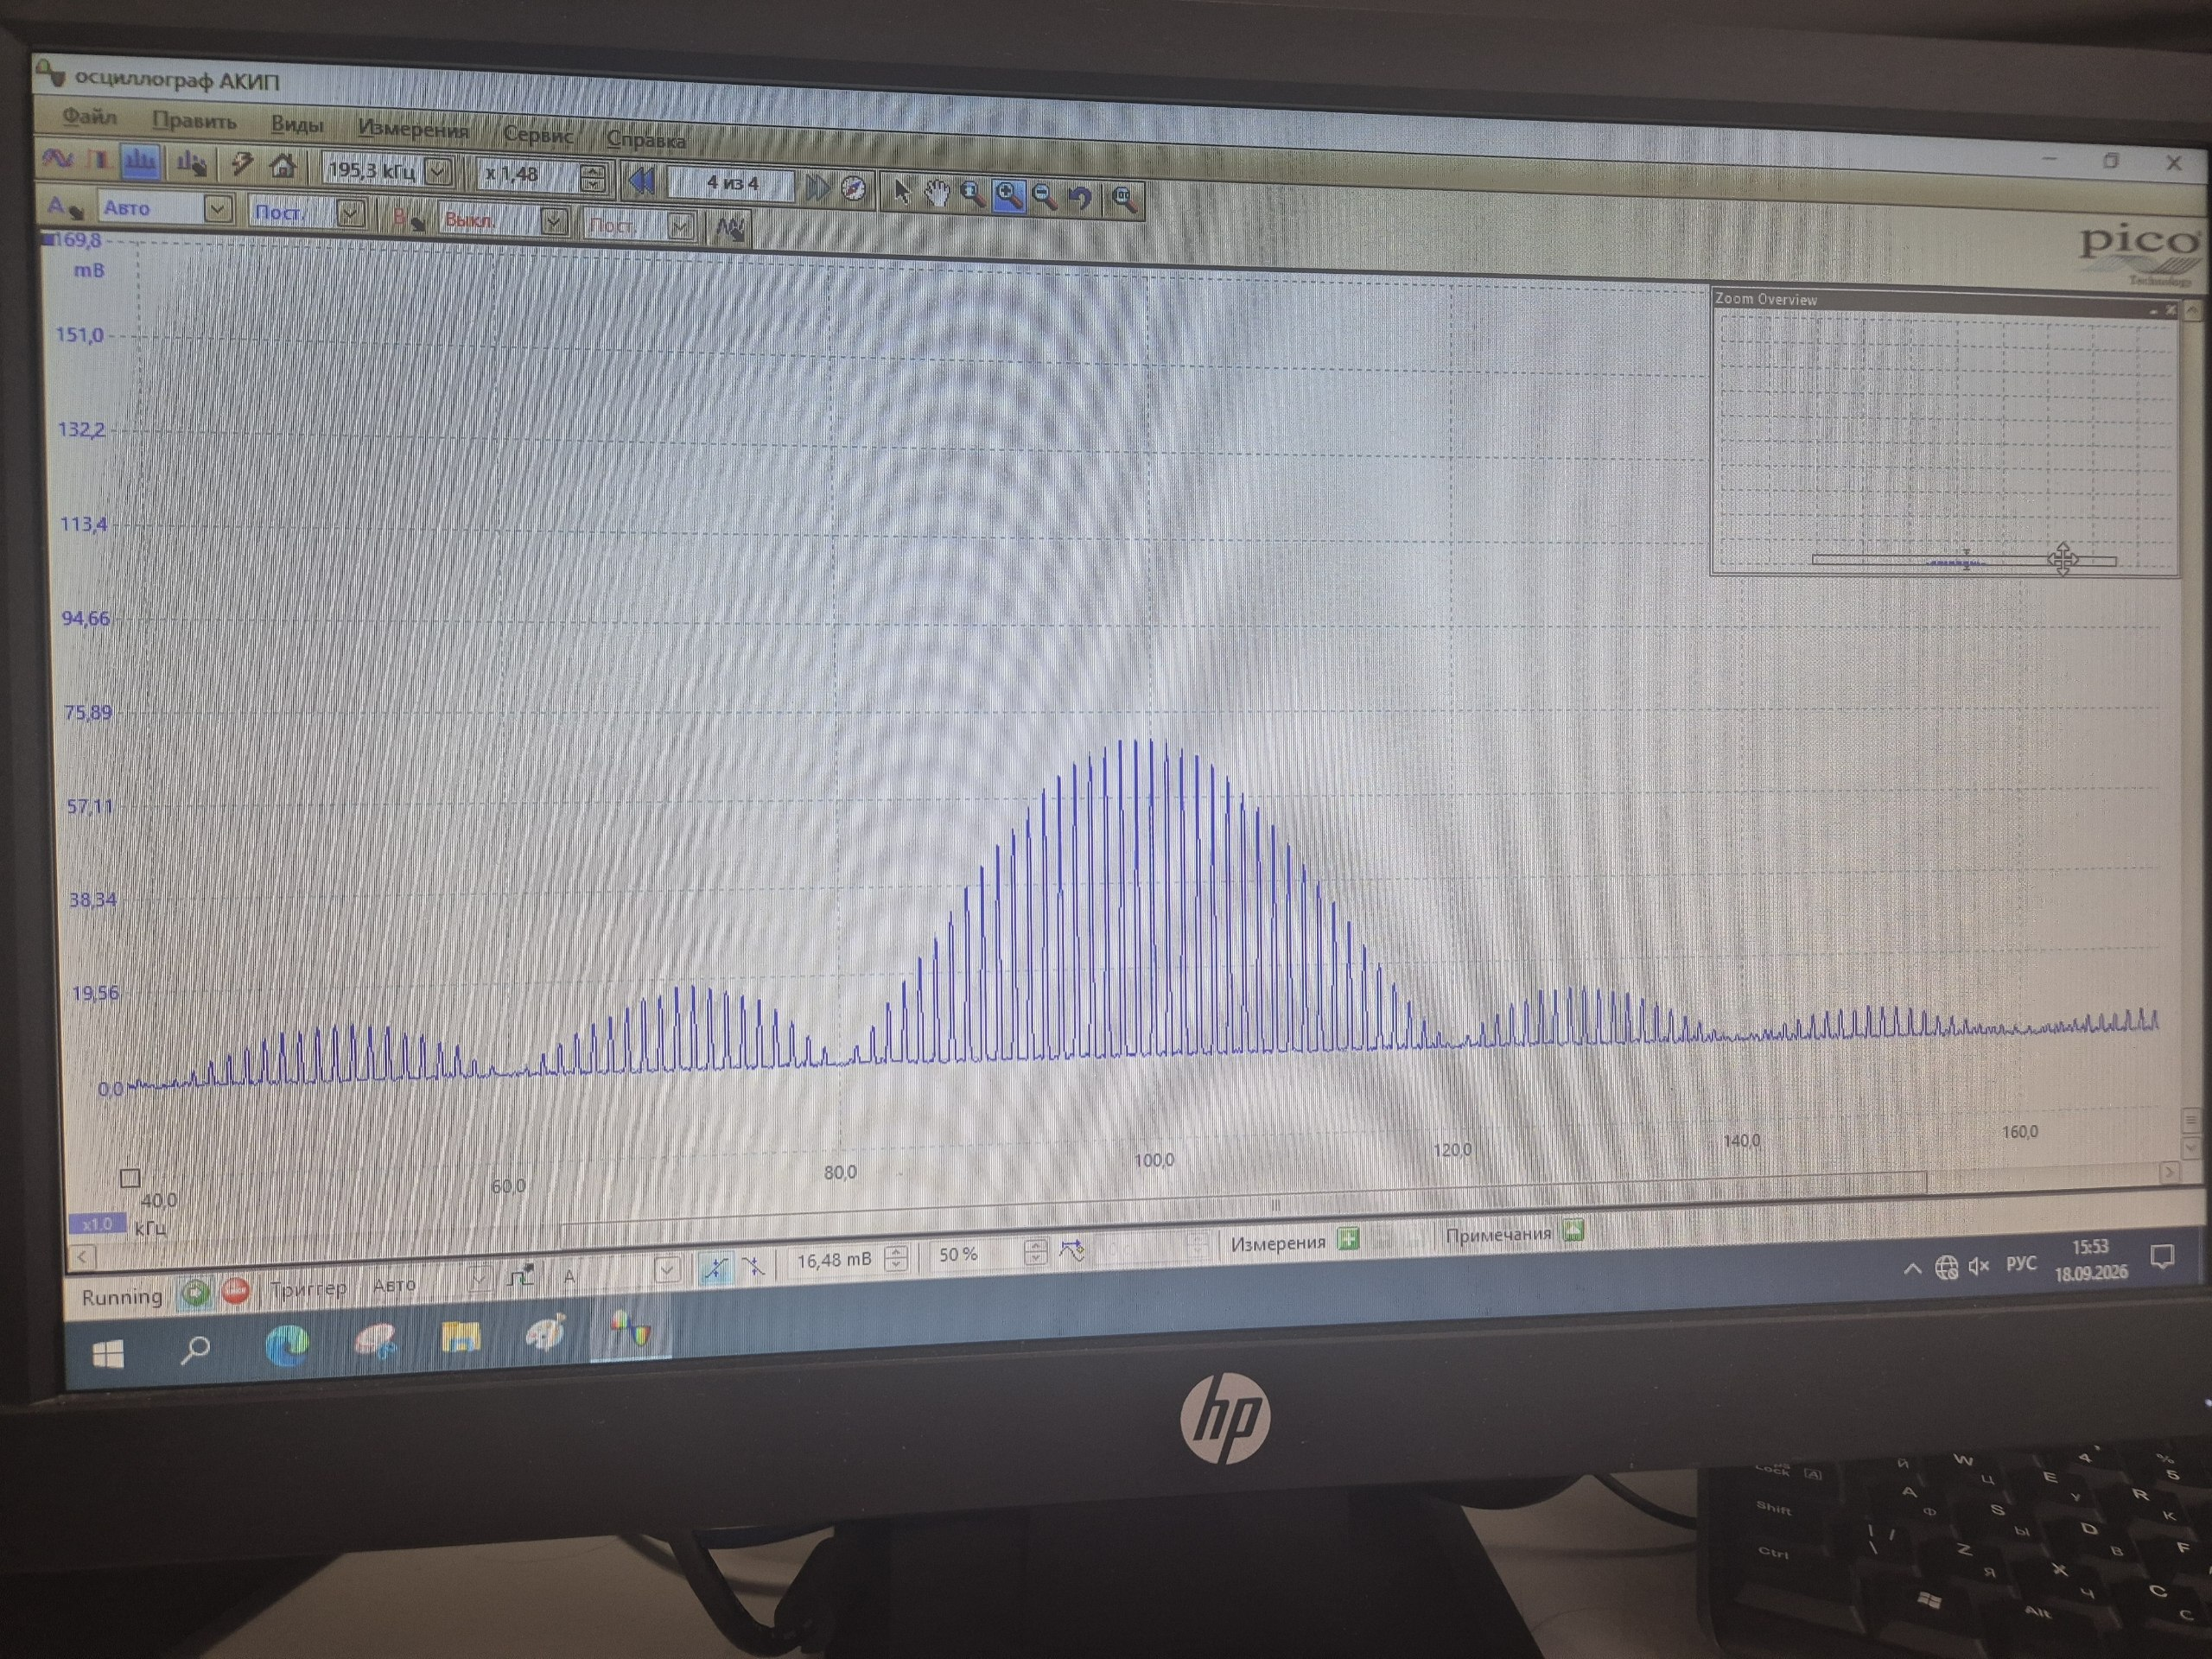
\includegraphics[width=\textwidth]{images/B_nu100.jpg}
        \caption{$\nu_0=100$ кГц}
    \end{subfigure}

    \vspace{0.5cm}

    \begin{subfigure}{0.40\textwidth}
        \centering
        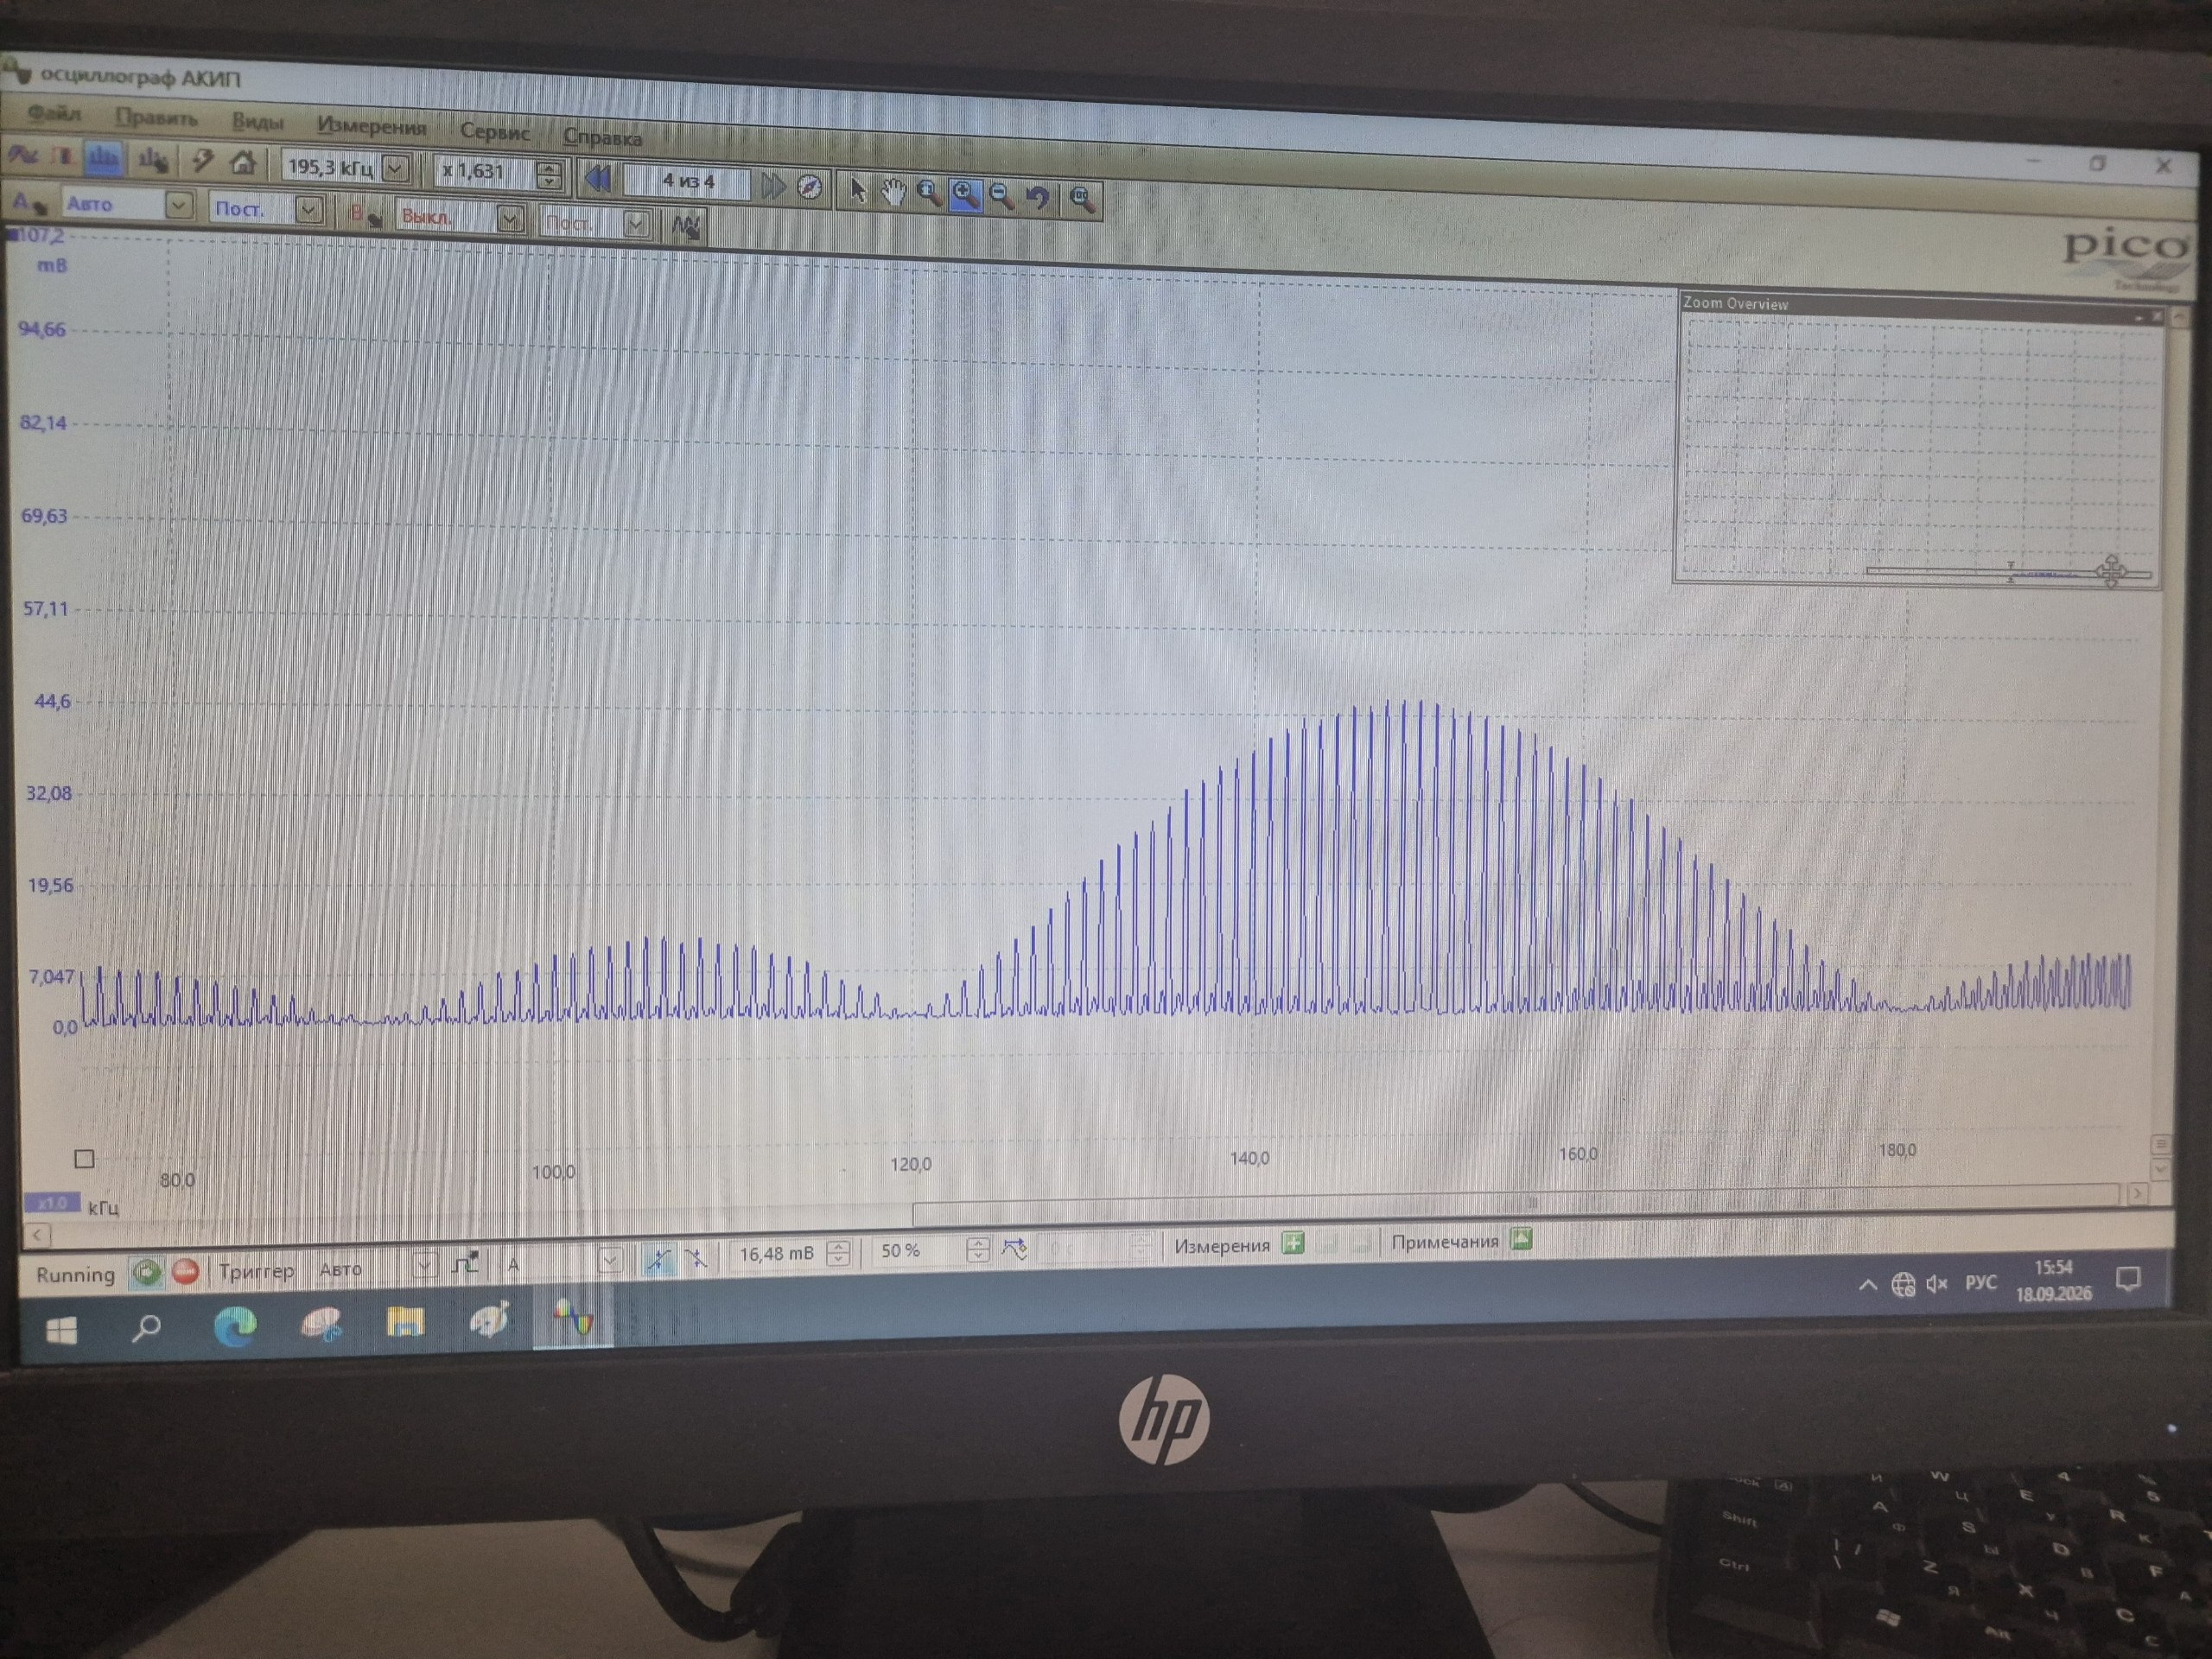
\includegraphics[width=\textwidth]{images/B_nu150.jpg}
        \caption{$\nu_0=150$ кГц}
    \end{subfigure}
    \hfill
    \begin{subfigure}{0.40\textwidth}
        \centering
        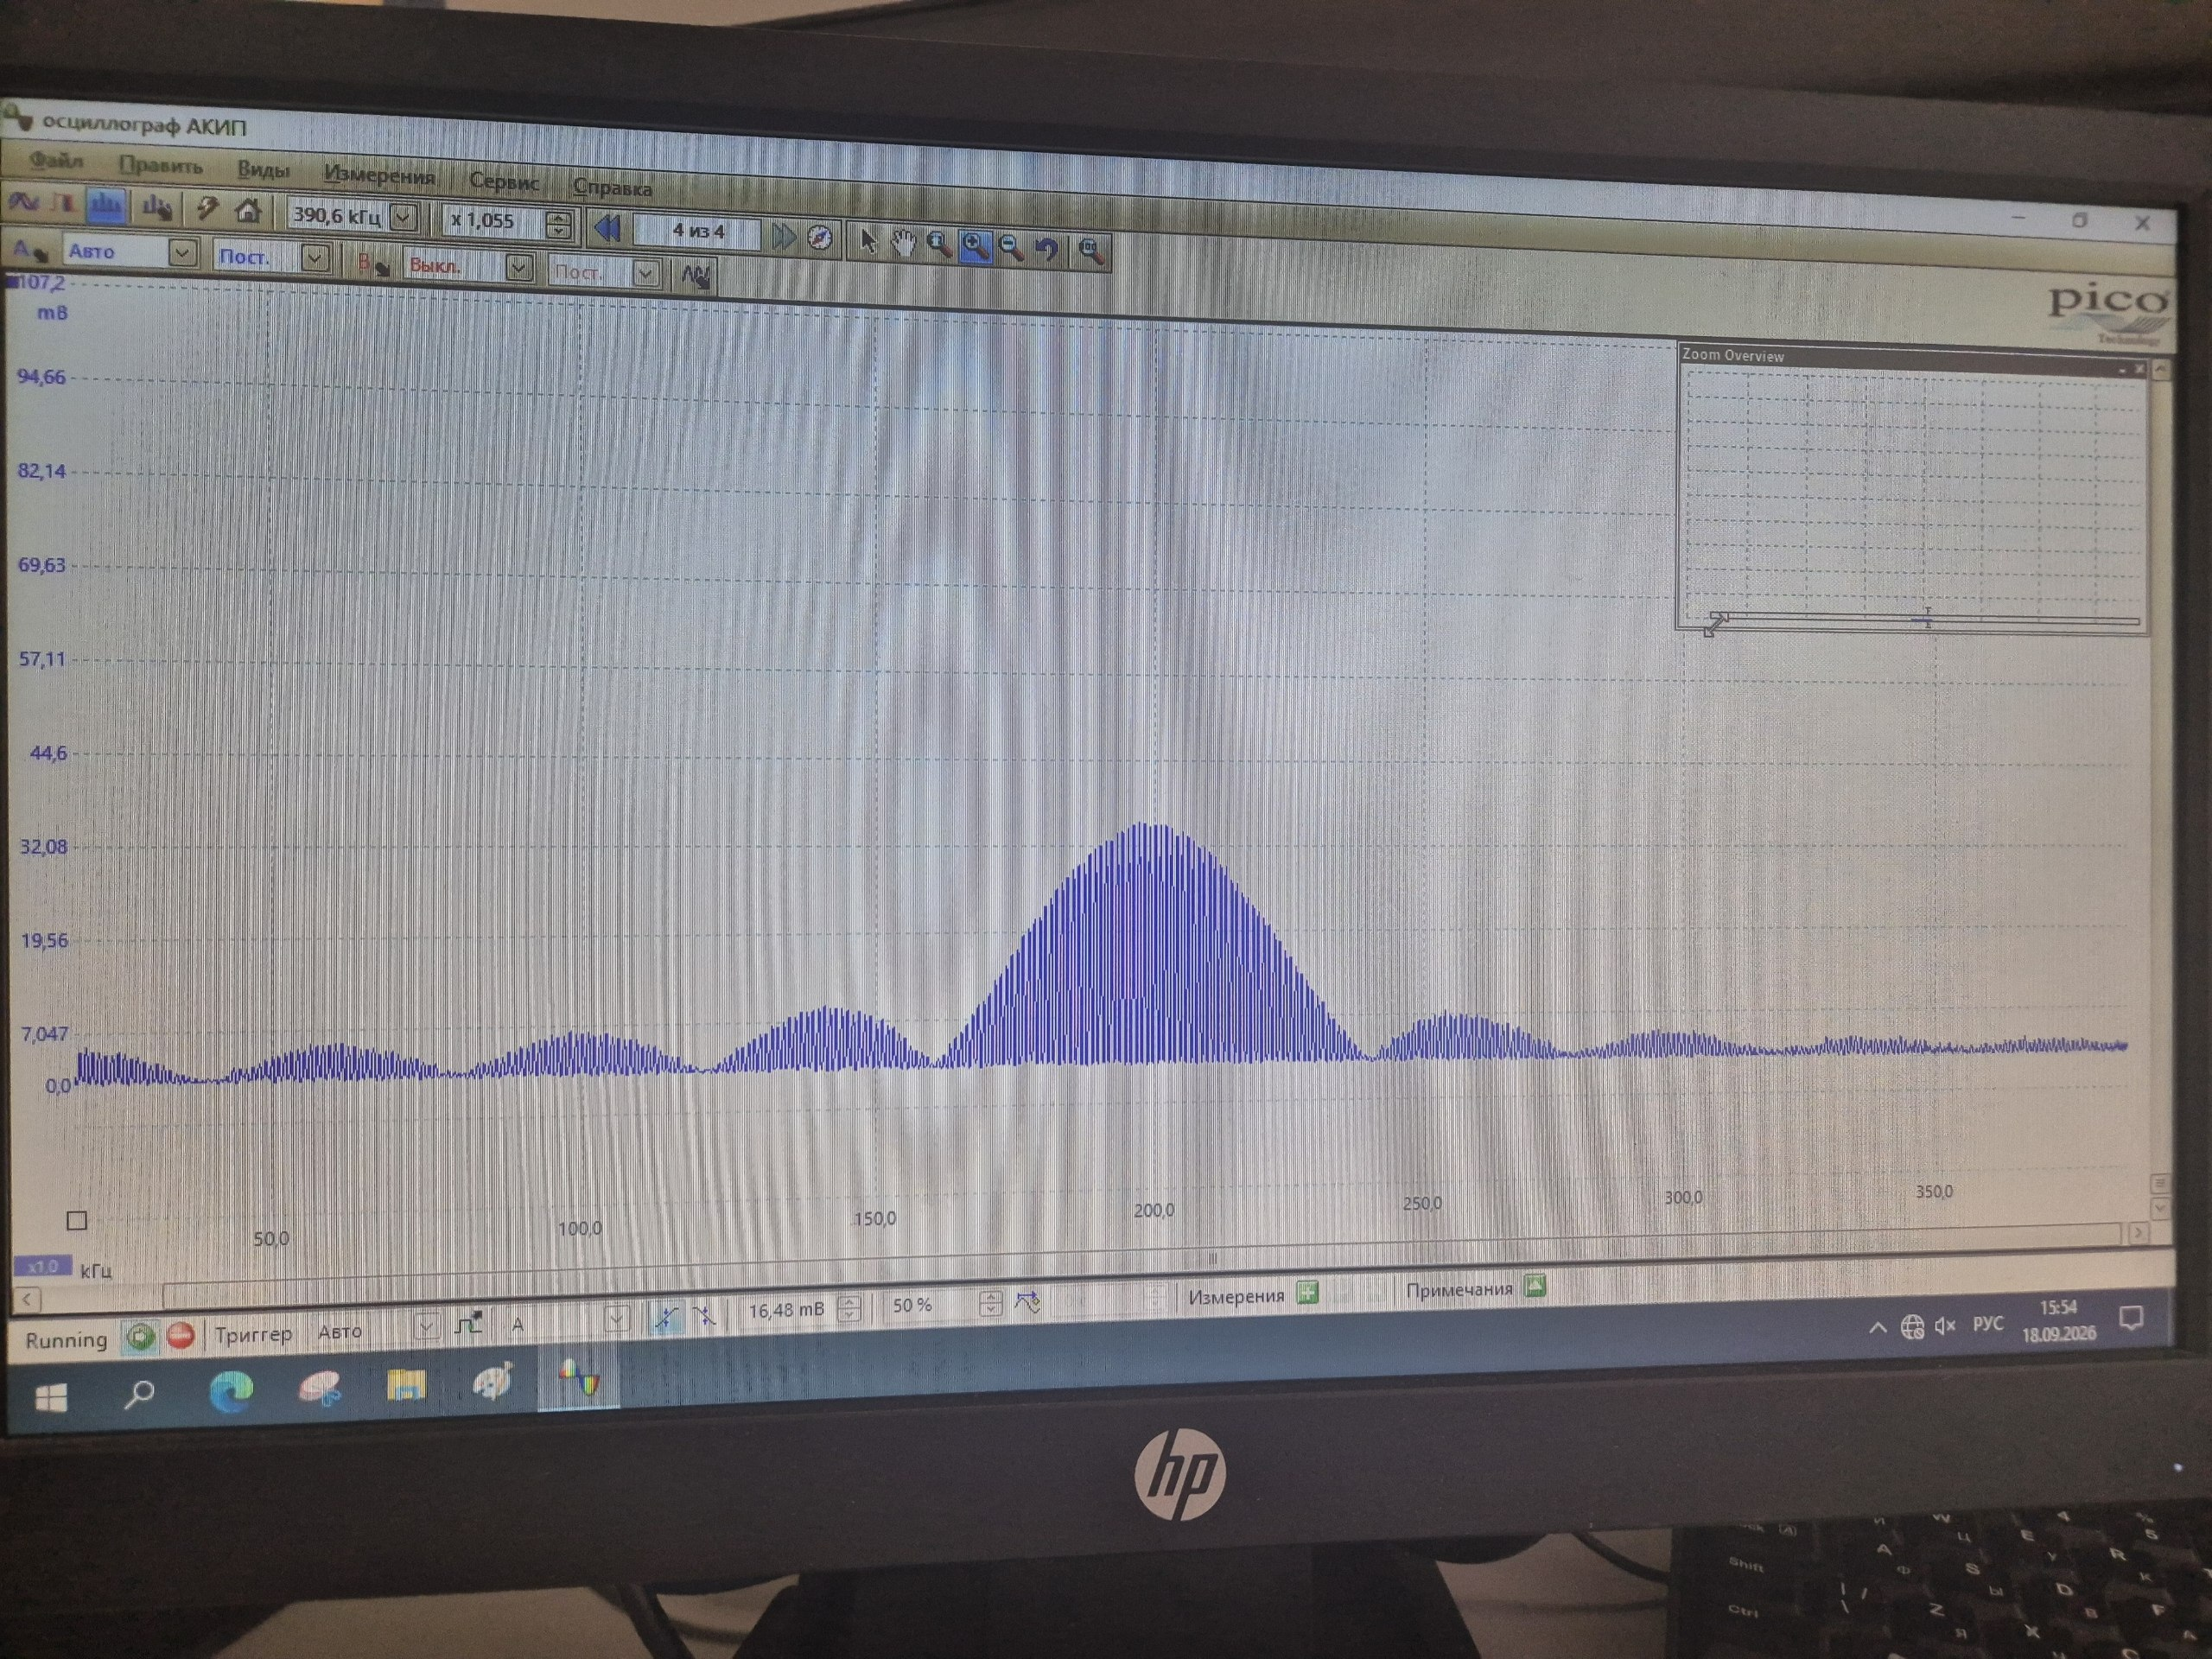
\includegraphics[width=\textwidth]{images/B_nu200.jpg}
        \caption{$\nu_0=200$ кГц}
    \end{subfigure}

    \caption{Спектры периодической последовательности цугов при
    различных значениях частоты заполнения $\nu_0$.}
\end{figure}

\subsection{Изменение параметров сигнала}

Исследовалось влияние параметров $\nu_0$, $T$ и $N$ на положение
и ширину спектральных компонент.

% TODO: таблица экспериментальных данных

\begin{table}[H]
\centering
\caption{Исследование спектра цугов}
\begin{tabular}{c|c|c|c|c}
$\nu_0$, кГц & $T$, мс & $N$ & $\Delta\nu$, кГц & $\delta\nu$, кГц \\
\hline
30 & 1 & 5 & 6.05 & 1.18\\
40 & 1 & 5 & 7.86 & 0.94\\
50 & 1 & 5 & 9.98 & 0.86\\
50 & 1 & 5 & 9.94 & 0.86\\
50 & 1 & 10 & 4.87 & 1.18\\
50 & 2 & 5 & 10.09 & 0.56\\
50 & 2 & 10 & 5.03 & 0.63
\end{tabular}
\end{table}

\subsection{Проверка теоремы смещения и соотношений неопределённостей}

\begin{table}[H]
    \centering
    \caption{Проверка теоремы смещения.}
    \begin{tabular}{c|c}
        \hline
        $\nu_0$, кГц & $\nu_{\text{ц}}$, кГц \\
        \hline
        50  & 50  \\
        100 & 100 \\
        150 & 150 \\
        200 & 200 \\
        \hline
    \end{tabular}
\end{table}

Из полученных спектров видно, что центральная частота спектра
совпадает с частотой заполнения:
\[
\nu_{\text{ц}}=\nu_0.
\]

Таким образом, эксперимент подтверждает справедливость теоремы
смещения.

\begin{figure}[H]
    \centering
    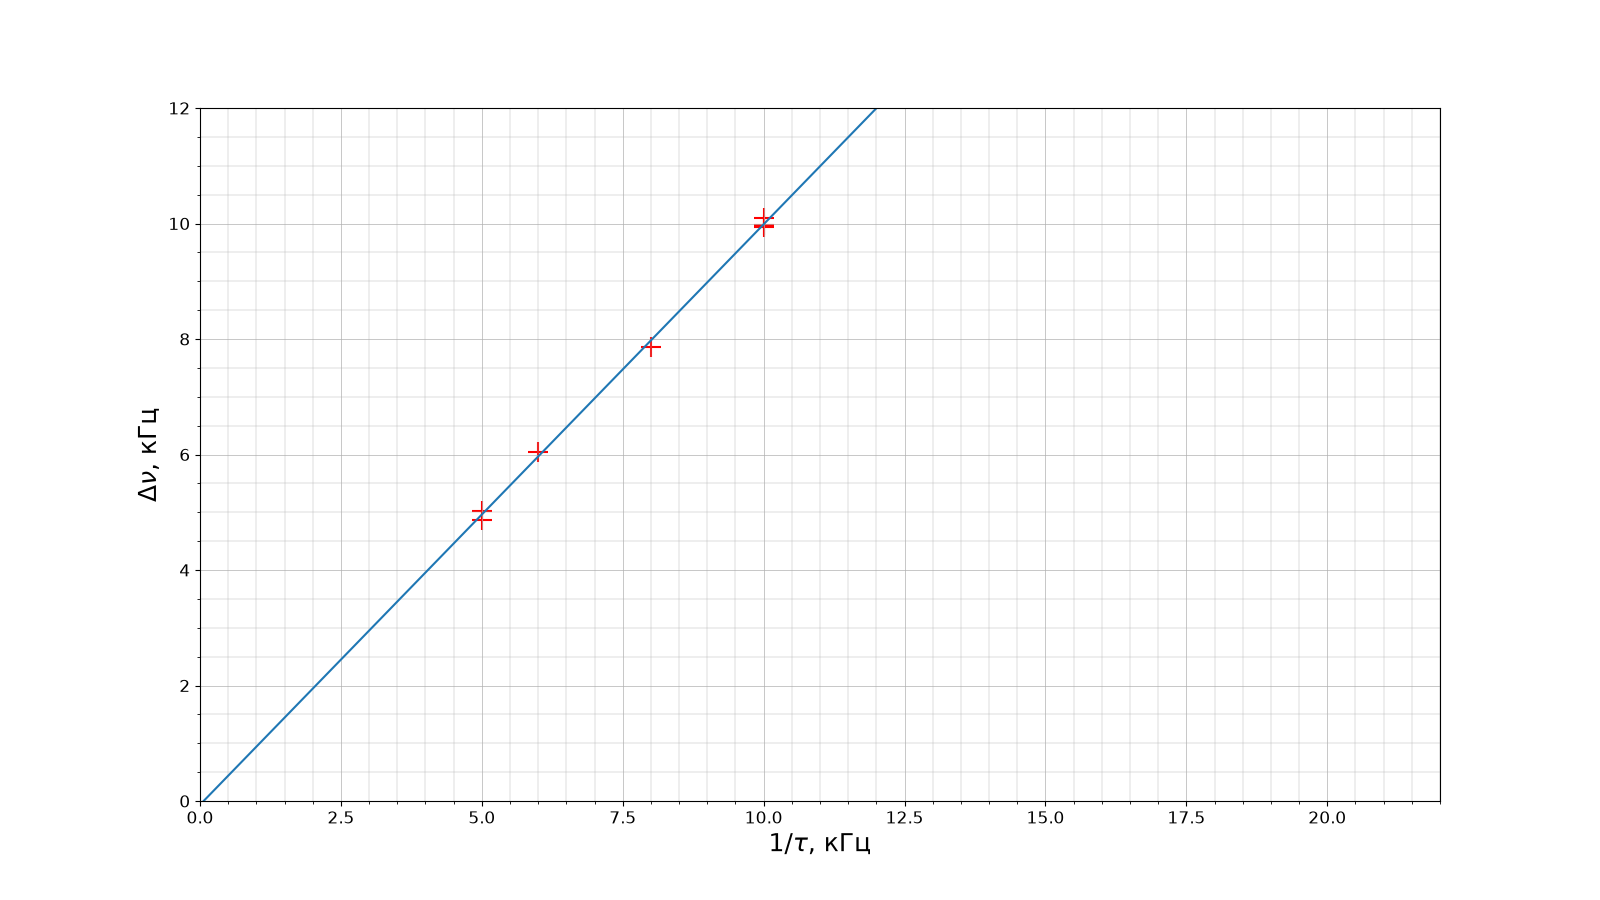
\includegraphics[width=1\textwidth]{images/delta_nu_1_tau_B.png}
    \caption{Зависимость ширины спектра $\Delta\nu$ от обратной длительности цуга $1/\tau$.}
    \label{fig:B_delta_nu_tau}
\end{figure}

Из графика получена линейная зависимость
\[
\Delta\nu = a\frac{1}{\tau}+b,
\]
где
\[
a=(1{.}005\pm0{.}017),
\qquad
b=(-0{.}065\pm0{.}134).
\]

Полученное значение коэффициента наклона согласуется с теоретическим
значением $a=1$. Следовательно, эксперимент подтверждает соотношение
неопределённостей
\[
\boxed{\Delta\nu\sim\frac{1}{\tau}}.
\]

\begin{figure}[H]
    \centering
    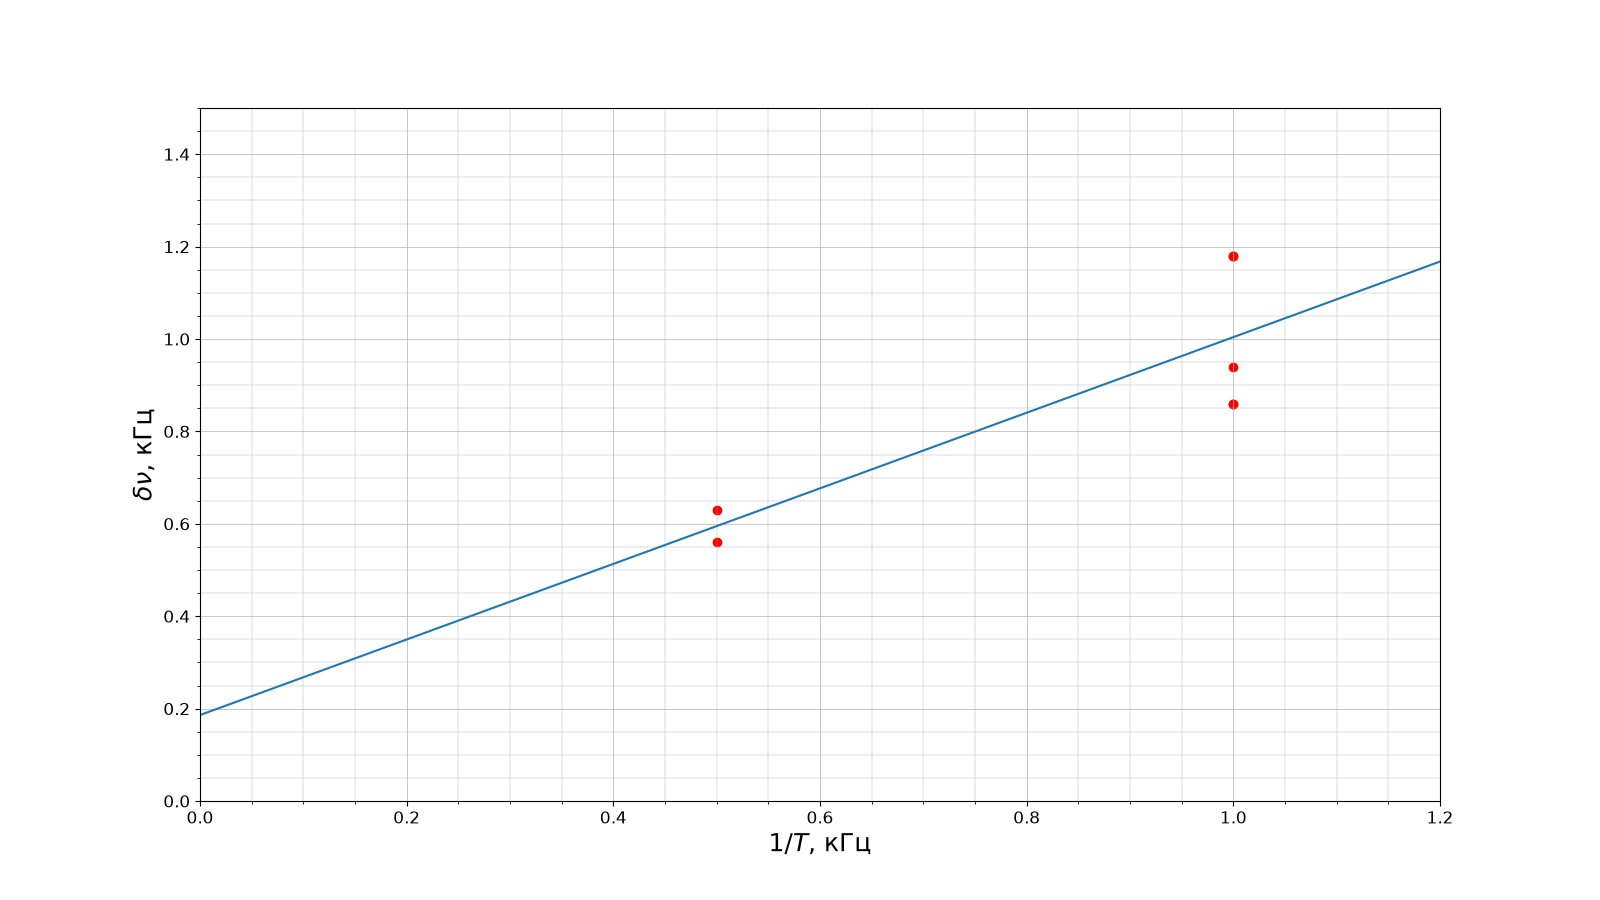
\includegraphics[width=1\textwidth]{images/delta_nu_1_T_B.png}
    \caption{Зависимость расстояния между соседними спектральными линиями
    $\delta\nu$ от обратного периода повторения цугов $1/T$.}
    \label{fig:B_delta_nu_T}
\end{figure}

Из графика получена линейная зависимость
\[
\delta\nu=a\frac{1}{T}+b,
\]
где
\[
a=(0{.}818\pm0{.}248),
\qquad
b=(0{.}186\pm0{.}220).
\]

Теоретическое значение коэффициента наклона равно
\[
a_{\text{теор}}=1.
\]

Полученное экспериментальное значение согласуется с теоретическим
в пределах погрешности:
\[
|1-0{.}818|=0{.}182<0{.}248.
\]

Следовательно, эксперимент подтверждает соотношение
неопределённостей
\[
\boxed{\delta\nu\sim\frac{1}{T}}.
\]

% =========================================================
% Г
% =========================================================

\section{Исследование спектра амплитудно-модулированного сигнала}

\subsection{Параметры сигнала}

Исследовался синусоидальный сигнал, модулированный по амплитуде.

% TODO: вписать фактические параметры эксперимента

\begin{table}[H]
\centering
\caption{Параметры амплитудно-модулированного сигнала}
\begin{tabular}{|c|c|}
\hline
Параметр & Значение \\
\hline
$\nu_0$ & 50 кГц\\
\hline
$\nu_{\text{мод}}$ & 2 кГц\\
\hline
$m$ & 0.5\\
\hline
\end{tabular}
\end{table}

\subsection{Исследование формы модулированного сигнала}

На экране осциллографа наблюдался амплитудно-модулированный
синусоидальный сигнал.

Измерялись максимальная $A_{\max}$ и минимальная $A_{\min}$
амплитуды сигнала.

Глубина амплитудной модуляции определяется выражением
\begin{equation}
m=
\frac{A_{\max}-A_{\min}}
     {A_{\max}+A_{\min}}.
\end{equation}

\begin{table}[H]
\centering
\caption{Измерение глубины модуляции}
\begin{tabular}{|c|c|c|c|}
\hline
$A_{\max}$ & $A_{\min}$ & $m_{\text{эксп}}$ & $m_{\text{зад}}$ \\
\hline
3.057 мВ& 1.027 мВ& 0.497& 0.500\\
\hline
\end{tabular}
\end{table}

\subsection{Зависимость отношения амплитуд от глубины модуляции}

Исследовалась зависимость отношения амплитуды боковой гармоники
к амплитуде основной гармоники от глубины модуляции:
\[
\frac{a_{\text{бок}}}{a_{\text{осн}}}.
\]

% TODO: заполнить после обработки данных

\begin{table}[H]
    \centering
    \caption{Зависимость отношения амплитуд от глубины модуляции.}
    \begin{tabular}{c|c|c}
        $m$, \% &
        $a_{\text{бок}}/a_{\text{осн}}$ (эксп.) &
        $a_{\text{бок}}/a_{\text{осн}}$ (теор.) \\
        \hline
        10  & 0.05 & 0.05 \\
        20  & 0.10 & 0.10 \\
        30  & 0.16 & 0.15 \\
        40  & 0.21 & 0.20 \\
        50  & 0.27 & 0.25 \\
        80  & 0.42 & 0.40 \\
        100 & 0.51 & 0.50 \\
    \end{tabular}
\end{table}
% TODO: добавить теоретическую зависимость после обработки

\begin{figure}[H]
    \centering
    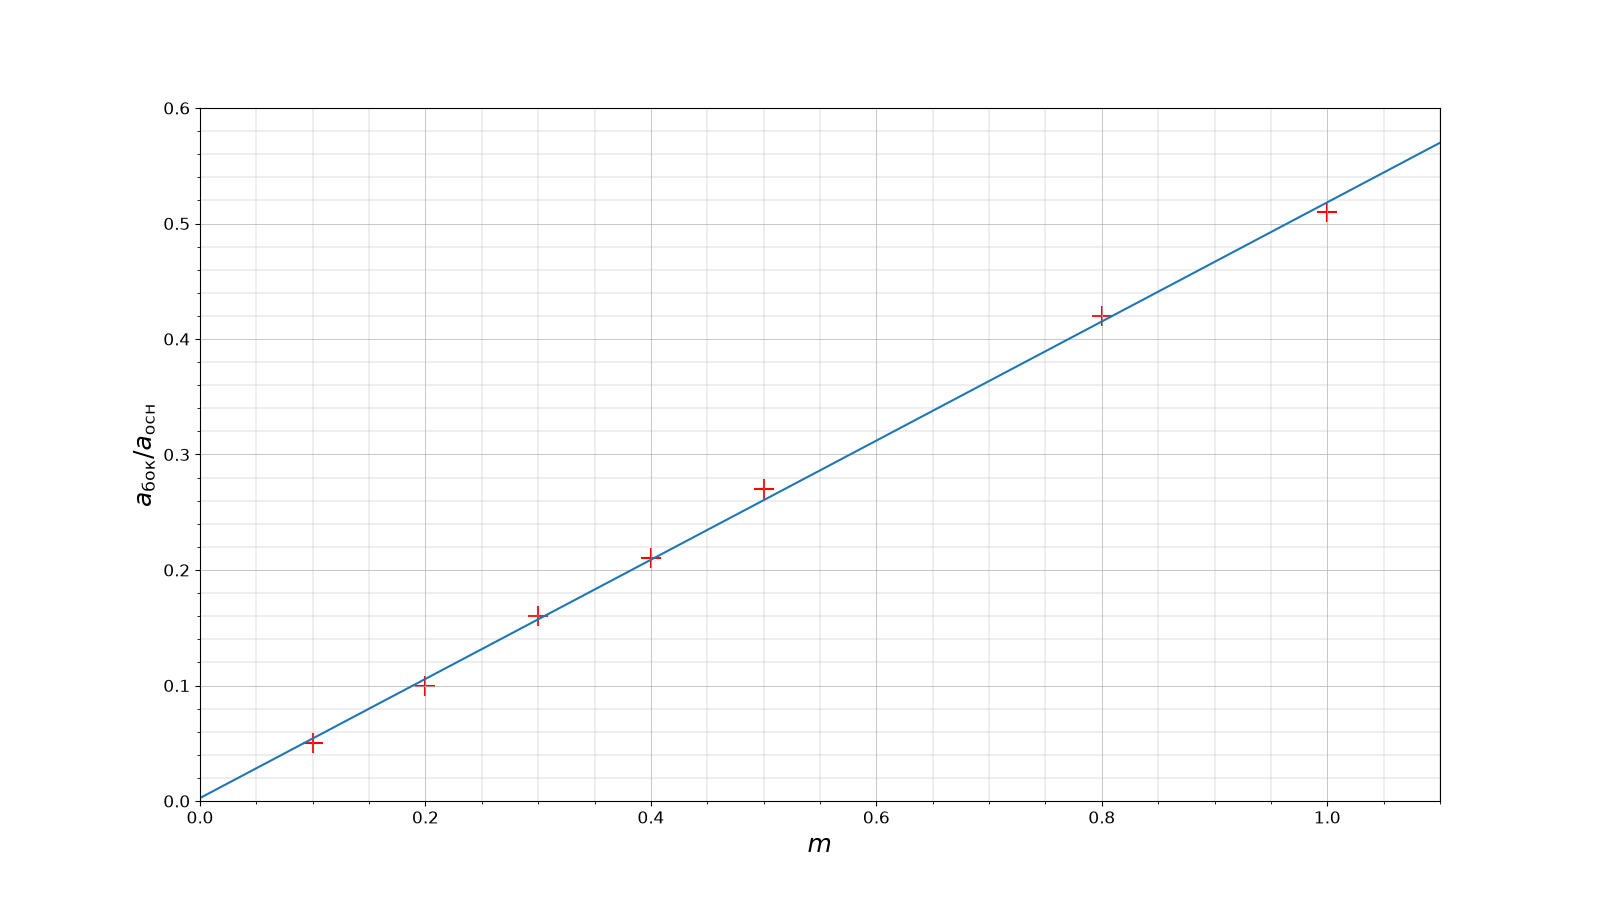
\includegraphics[width=0.8\textwidth]{images/amplitude_ratio_m.png}
    \caption{Зависимость отношения амплитуд боковой и основной линий
спектра от глубины модуляции.}
\end{figure}

Из графика получена линейная зависимость
\[
\frac{a_{\text{бок}}}{a_{\text{осн}}}
=
a m+b,
\]
где
\[
a=(0{.}516\pm0{.}009),
\qquad
b=(0{.}0026\pm0{.}0049).
\]

Теоретическая зависимость имеет вид
\[
\frac{a_{\text{бок}}}{a_{\text{осн}}}=\frac{m}{2},
\]
поэтому теоретическое значение коэффициента наклона равно
\[
a_{\text{теор}}=0{.}5.
\]

Экспериментальное значение коэффициента наклона близко к
теоретическому, что подтверждает линейную зависимость отношения
амплитуд боковой и основной линий от глубины модуляции.

% =========================================================
% Е
% =========================================================

\section{Изучение фильтрации сигналов}

\subsection{Теоретические сведения}

Для RC-фильтра нижних частот характерное время определяется выражением
\begin{equation}
\tau_{RC}=RC,
\end{equation}

а соответствующая характерная частота:
\begin{equation}
\nu_{RC}=\frac{1}{\tau_{RC}}.
\end{equation}

% TODO: вписать R и C

\begin{table}[H]
\centering
\caption{Параметры RC-цепочки}
\begin{tabular}{|c|c|}
\hline
Параметр & Значение \\
\hline
$R$ & 3 кОм\\
\hline
$C$ & 1000 пФ\\
\hline
$\tau_{RC}=RC$ & 3 мкс\\
\hline
$\nu_{RC}=1/\tau_{RC}$ & 333 кГц\\
\hline
\end{tabular}
\end{table}

\subsection{Наблюдение фильтрации}

На вход RC-цепочки подавалась последовательность прямоугольных
импульсов. Исследовались форма сигнала и его спектр на выходе
фильтра при различных периодах повторения.

При $T=3~\text{мкс}$ наблюдались следующие форма сигнала и его спектр:

\begin{figure}[H]
    \centering

    \begin{subfigure}{0.48\textwidth}
        \centering
        
\includegraphics[width=\textwidth]{images/1.jpg}
        \caption{Сигнал на выходе RC-фильтра.}
    \end{subfigure}
    \hfill
    \begin{subfigure}{0.48\textwidth}
        \centering
        
\includegraphics[width=\textwidth]{images/2.jpg}
        \caption{Спектр сигнала после RC-фильтра.}
    \end{subfigure}

    \caption{Сигнал и спектр при $T=3~\text{мкс}$.}
\end{figure}

\newpage

При $T=4~\text{мкс}$:

\begin{figure}[H]
    \centering

    \begin{subfigure}{0.48\textwidth}
        \centering
        
\includegraphics[width=\textwidth]{images/3.jpg}
        \caption{Сигнал на выходе RC-фильтра.}
    \end{subfigure}
    \hfill
    \begin{subfigure}{0.48\textwidth}
        \centering
        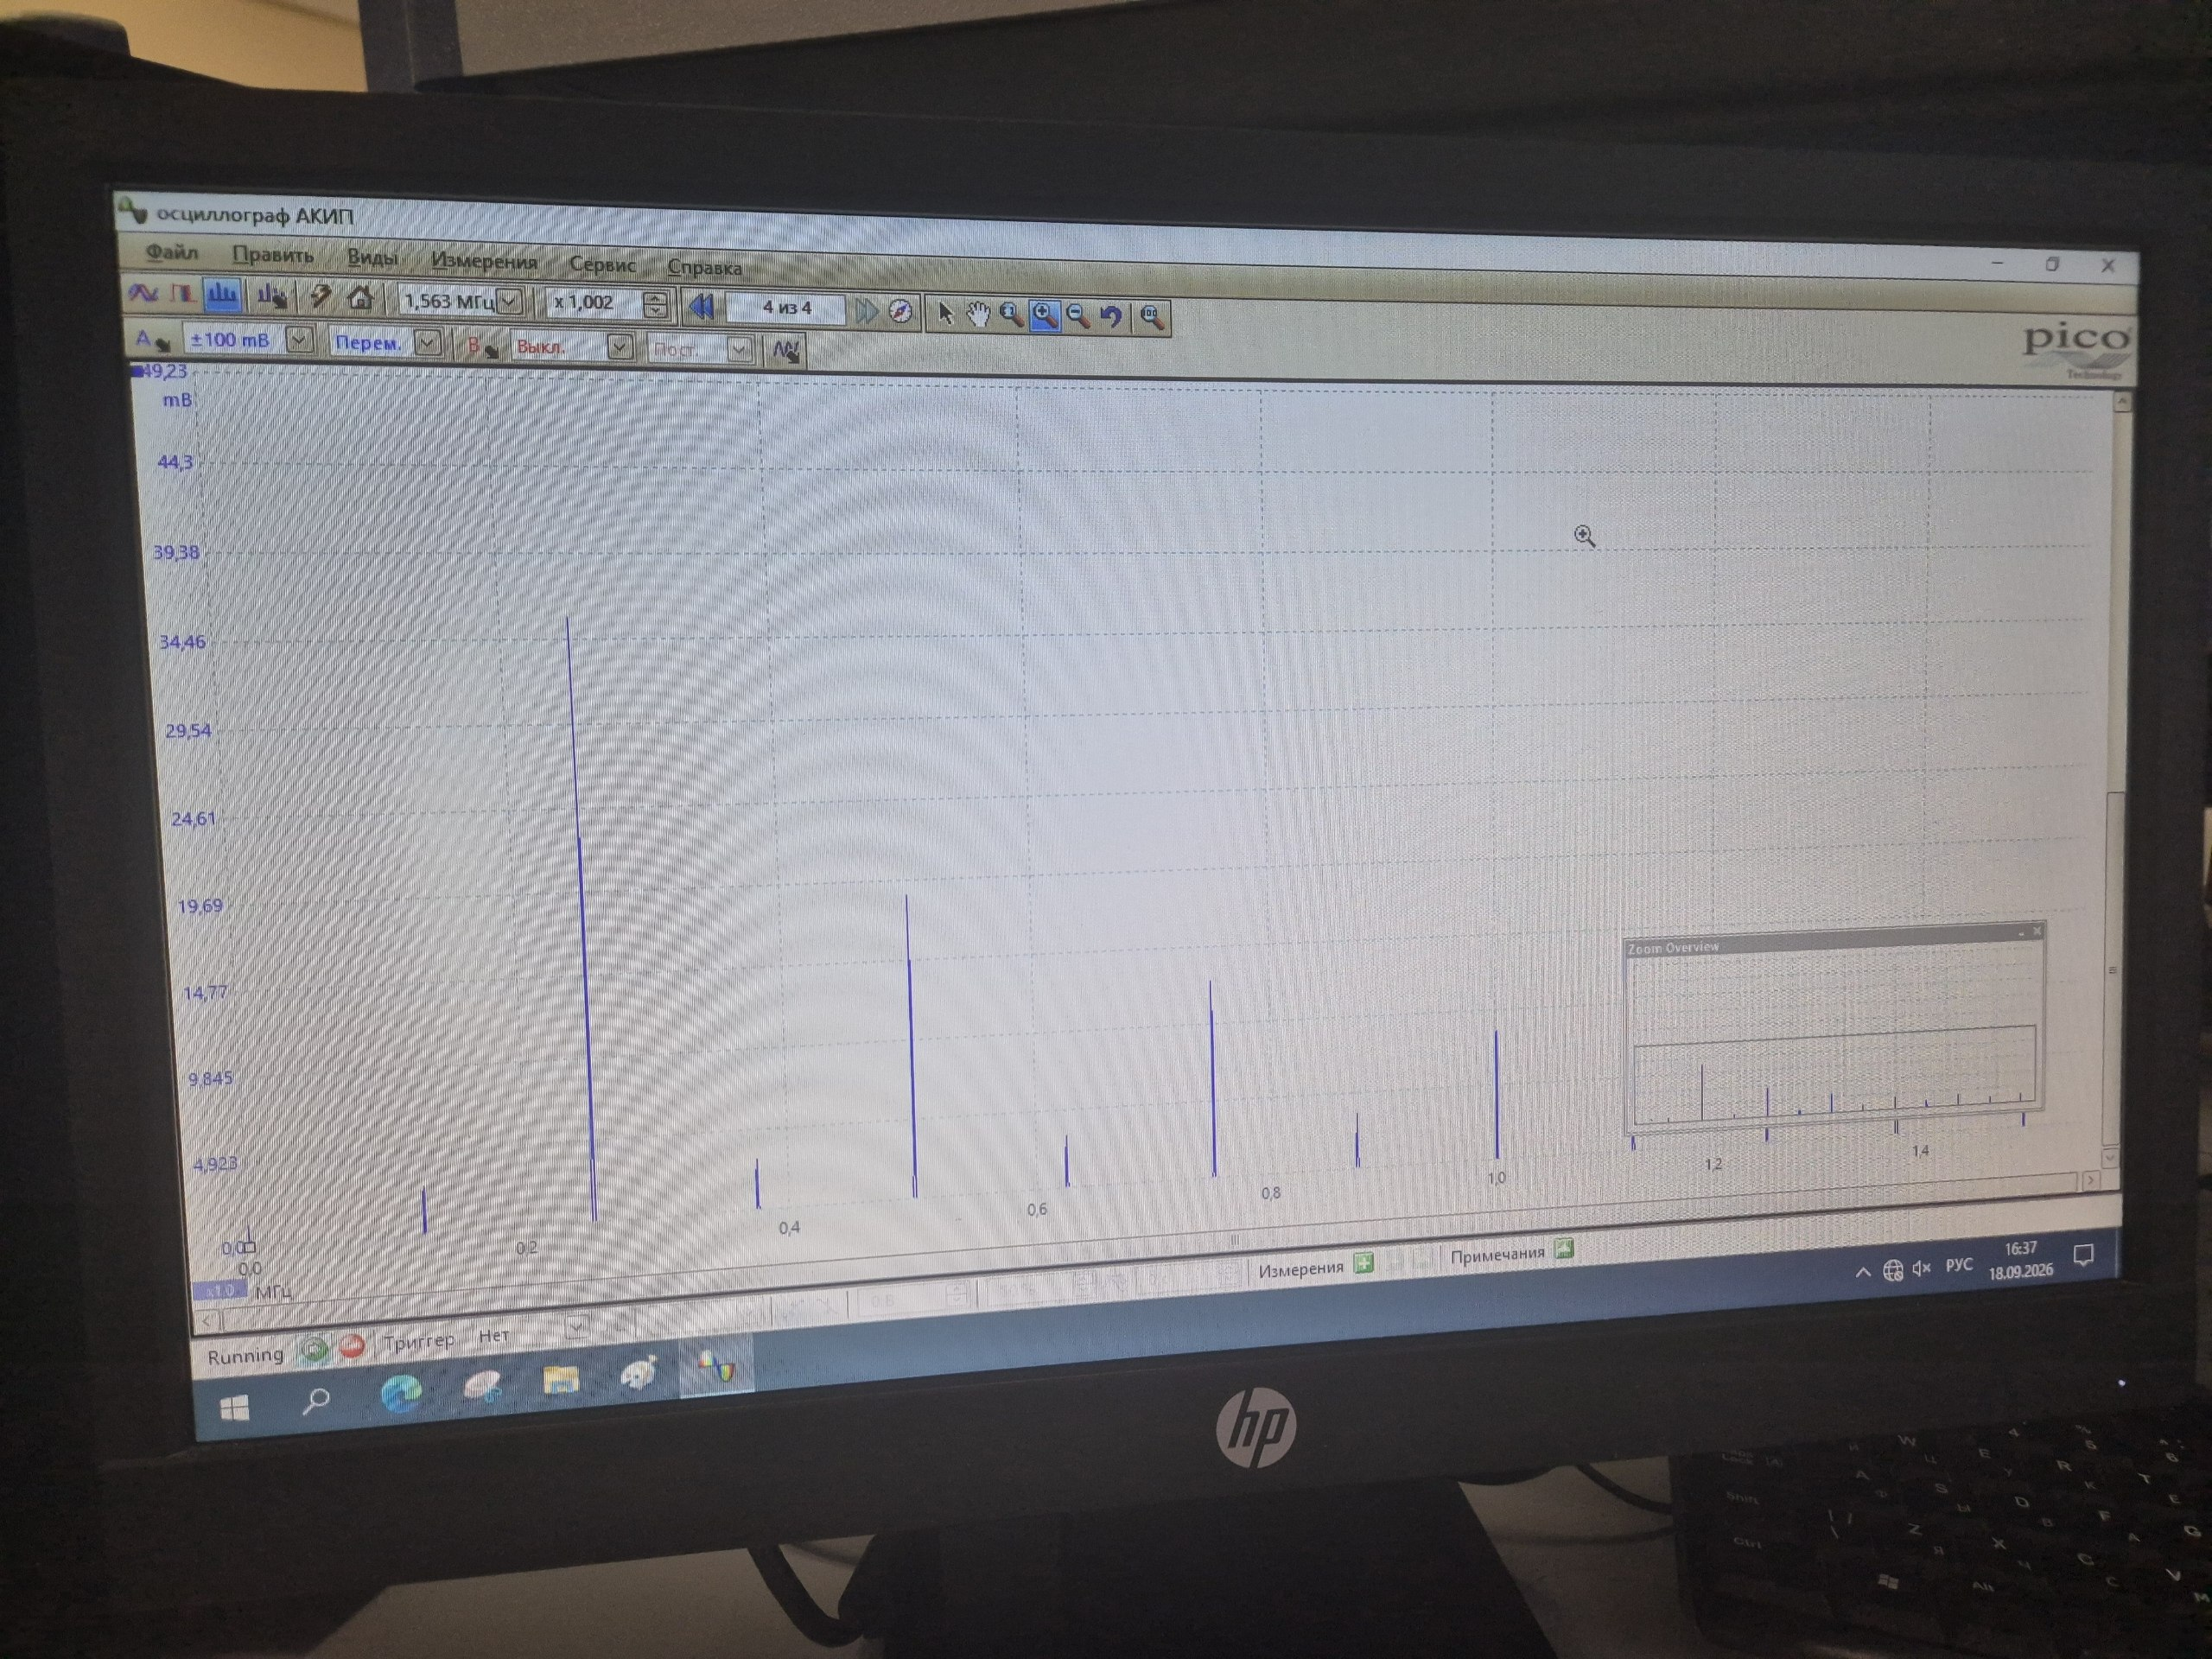
\includegraphics[width=\textwidth]{images/4.jpg}
        \caption{Спектр сигнала после RC-фильтра.}
    \end{subfigure}

    \caption{Сигнал и спектр при $T=4~\text{мкс}$.}
\end{figure}


При $T=10~\text{мкс}$:

\begin{figure}[H]
    \centering

    \begin{subfigure}{0.48\textwidth}
        \centering
        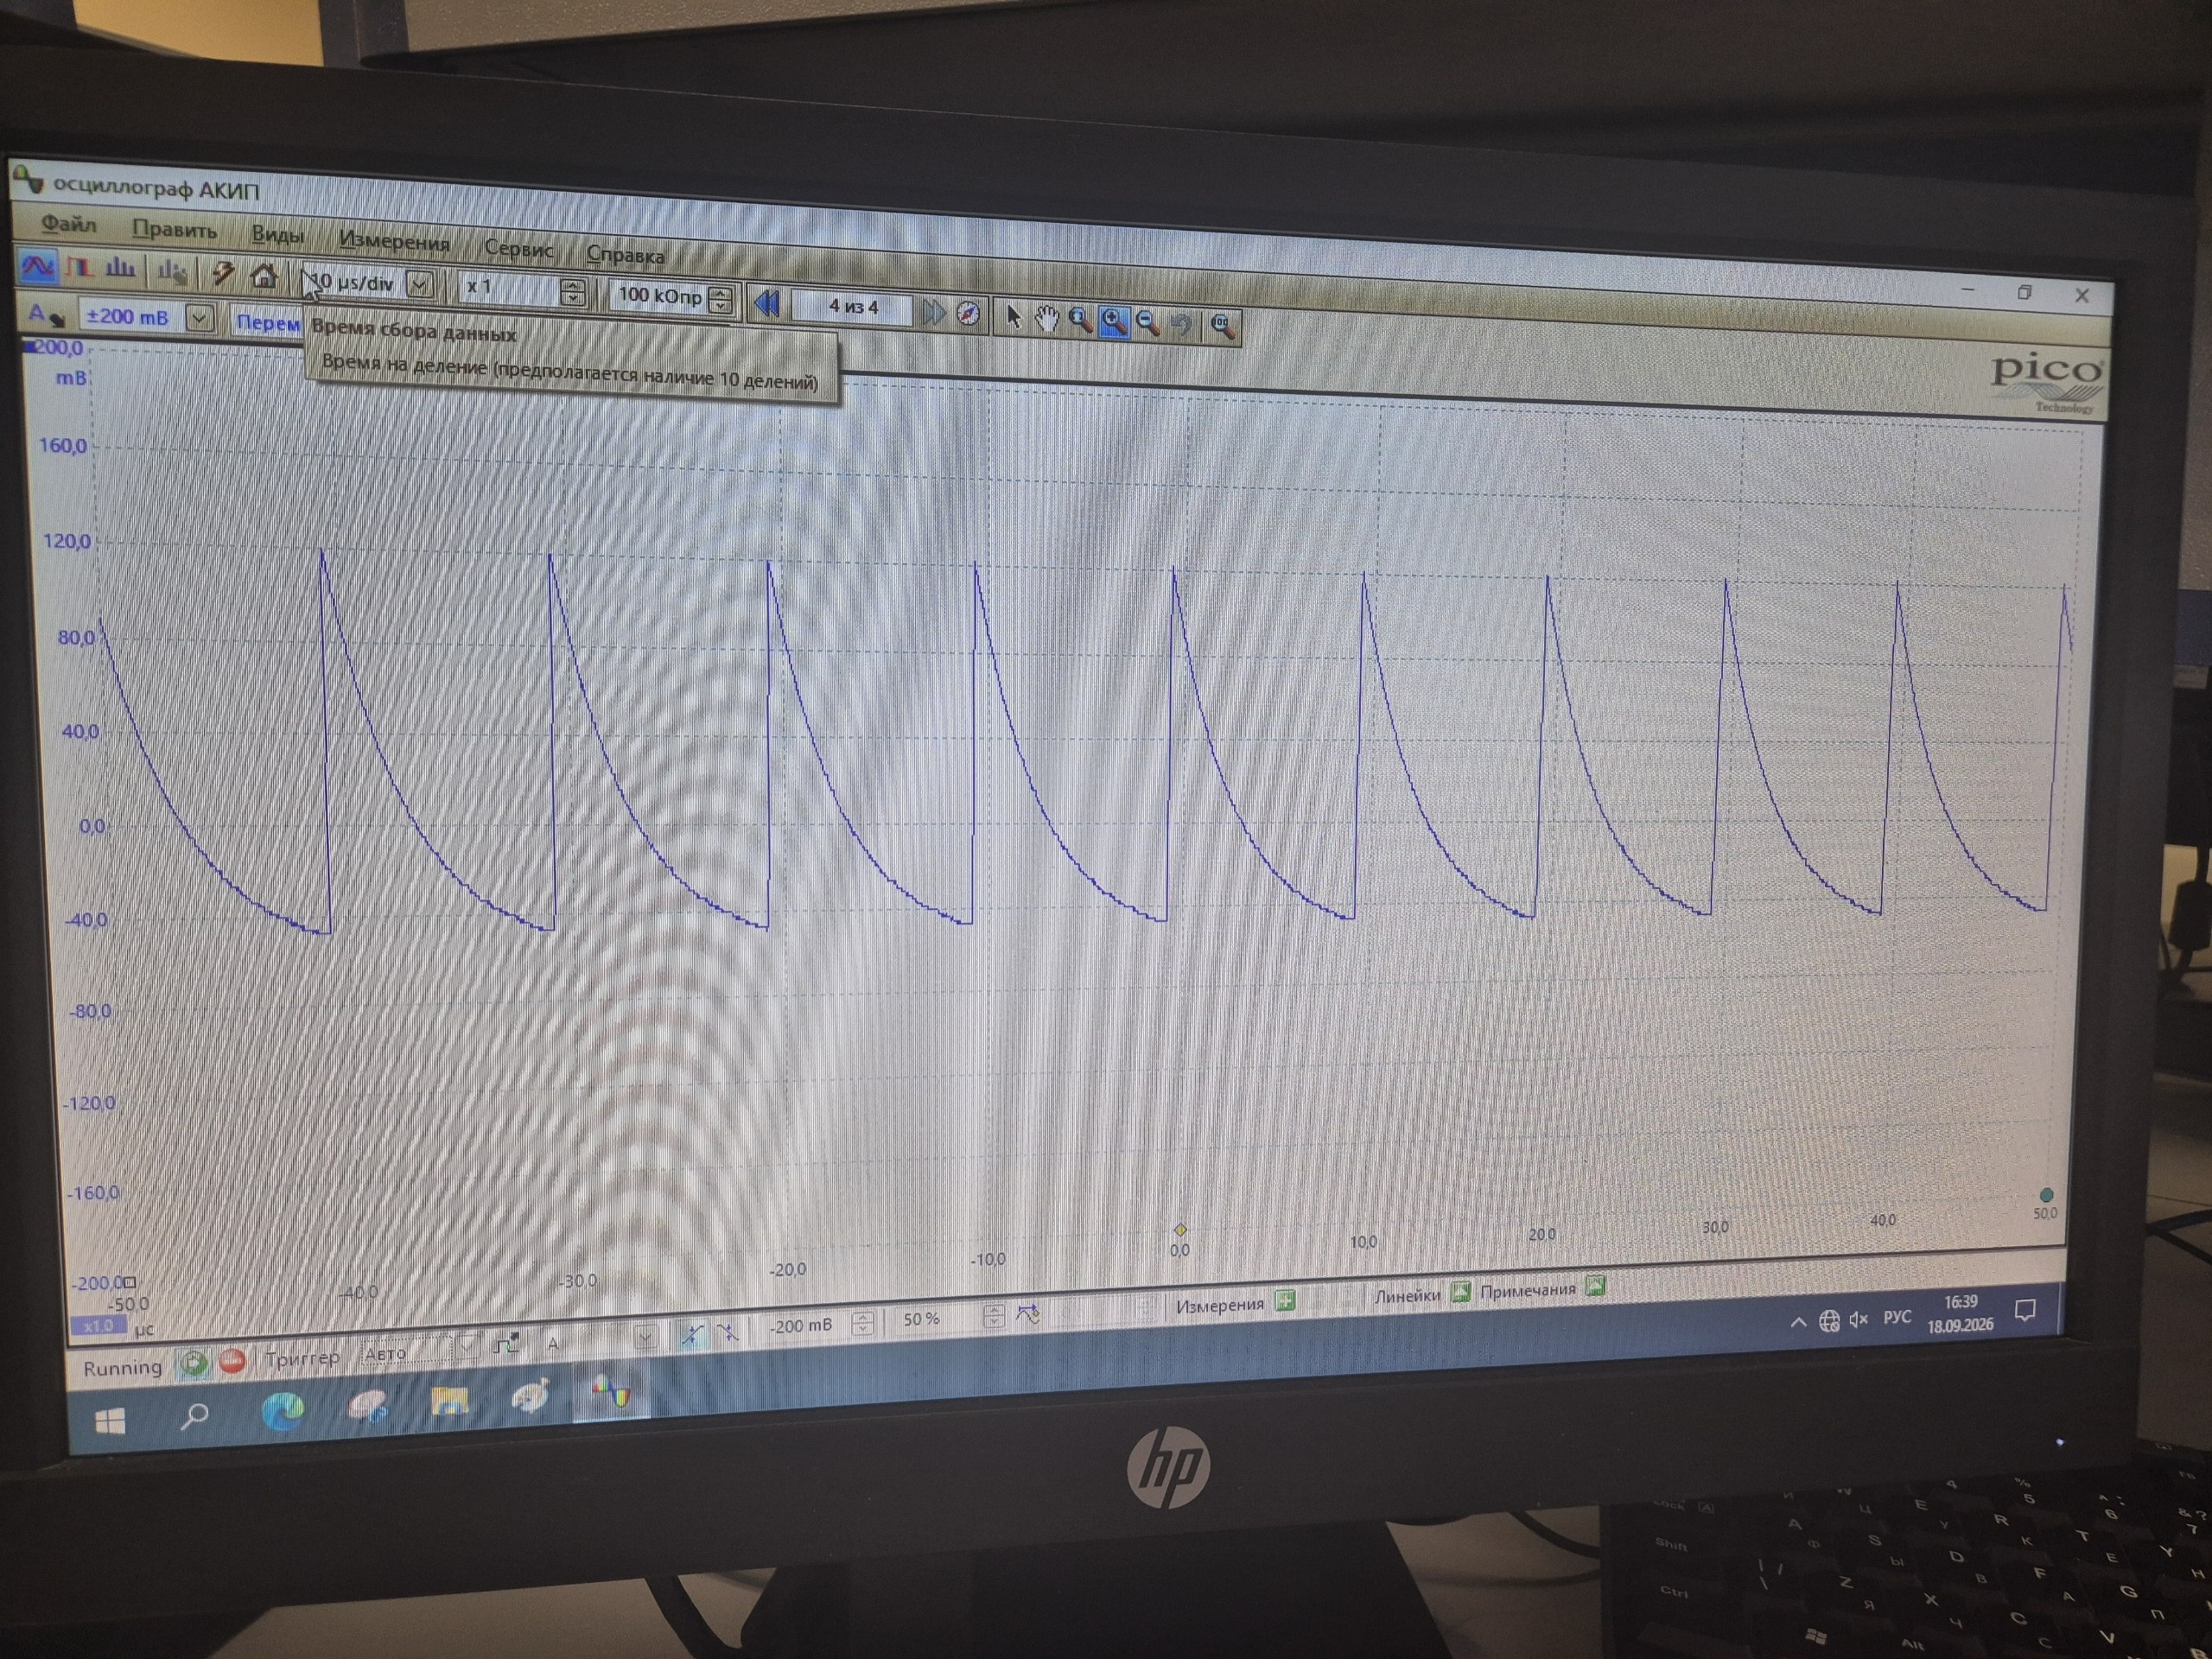
\includegraphics[width=\textwidth]{images/5.jpg}
        \caption{Сигнал на выходе RC-фильтра.}
    \end{subfigure}
    \hfill
    \begin{subfigure}{0.48\textwidth}
        \centering
        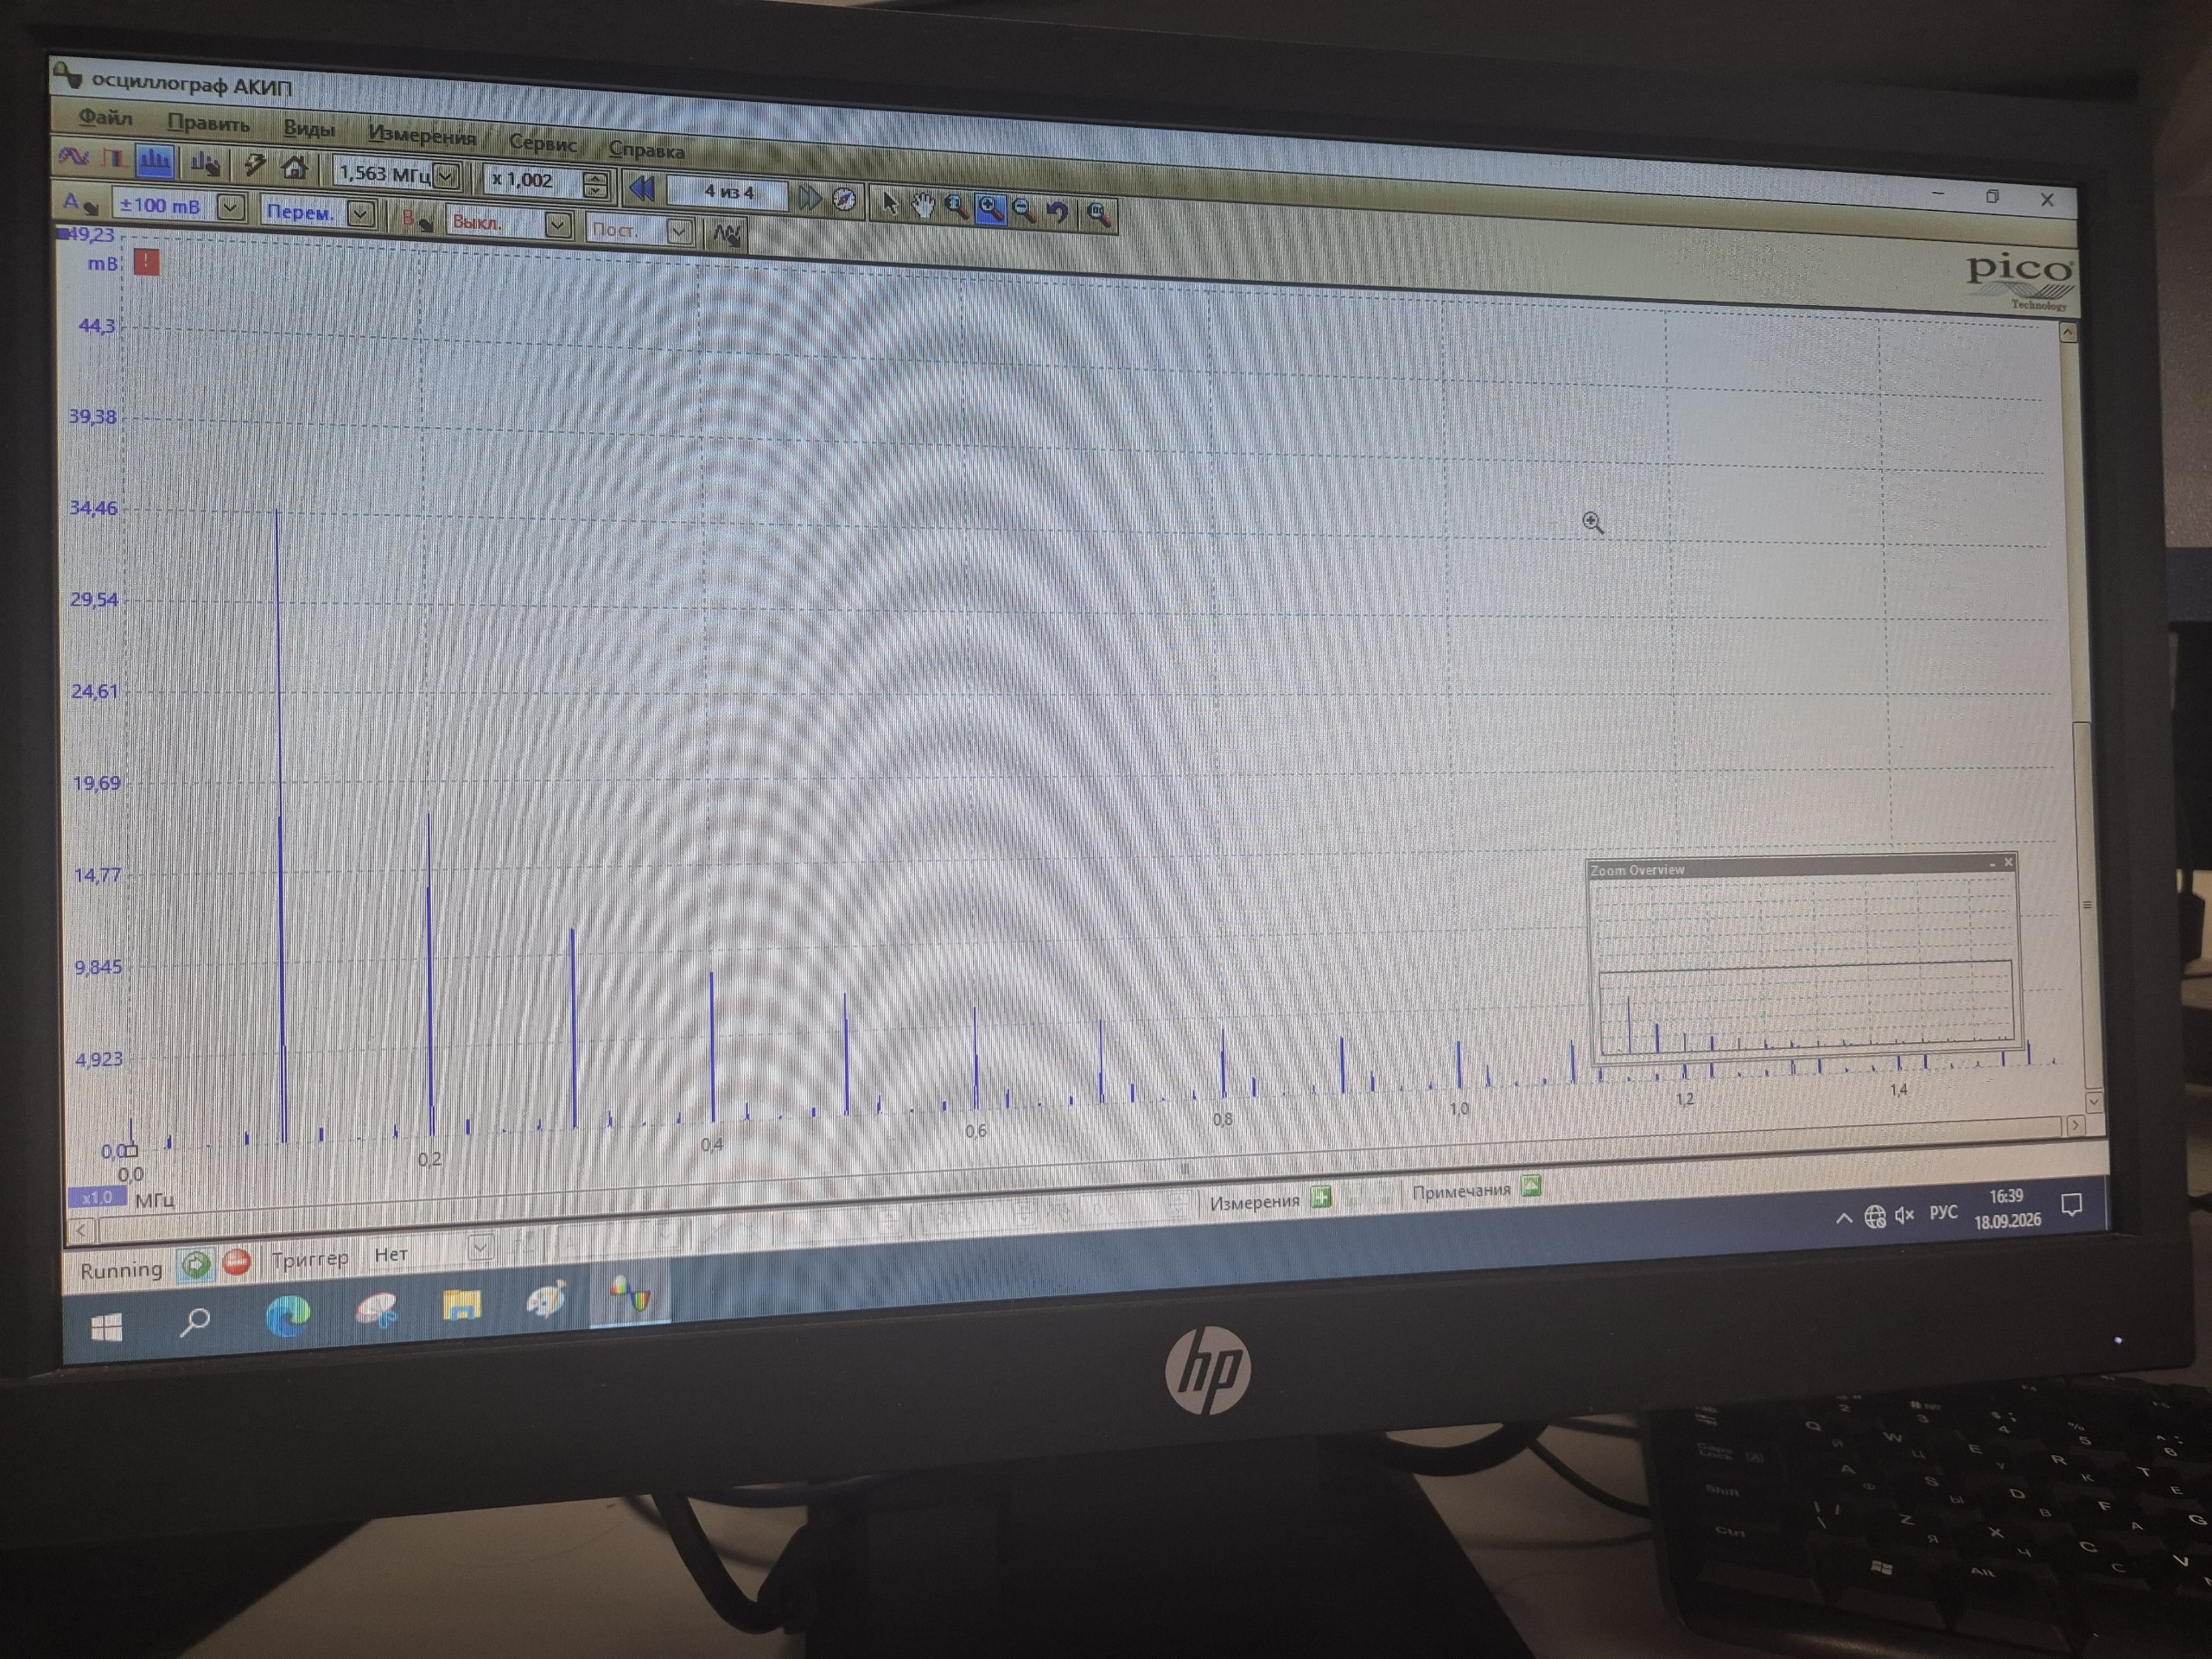
\includegraphics[width=\textwidth]{images/6.jpg}
        \caption{Спектр сигнала после RC-фильтра.}
    \end{subfigure}

    \caption{Сигнал и спектр при $T=10~\text{мкс}$.}
\end{figure}

При уменьшении периода повторения импульсов расстояние между
соседними спектральными линиями увеличивается. Это соответствует
теоретическому соотношению
\[
\delta\nu=\frac{1}{T}.
\]

Кроме того, RC-фильтр подавляет высокочастотные гармоники сигнала,
в результате чего форма сигнала на выходе становится близкой к
экспоненциально спадающему участку между соседними импульсами.

\subsection{Измерение коэффициента фильтрации}

Для нескольких спектральных гармоник определялся коэффициент фильтрации
\begin{equation}
K_n=
\frac{|a_n^{\text{ф}}|}
{|a_n^0|},
\end{equation}

где $a_n^{\text{ф}}$ --- амплитуда гармоники после фильтра,
$a_n^0$ --- амплитуда соответствующей гармоники исходного сигнала.

\begin{table}[H]
\centering
\caption{Измеренные параметры фильтрации}
\begin{tabular}{c|c|c}
$n$ & $|a_n^{0}|$, мВ & $|a_n^{\text{ф}}|$, мВ \\
\hline
1 & 4452& 695.0 \\
2 & 3768& 295.4 \\
3 & 3151& 166.6 \\
4 & 1991& 82.2 \\
5 & 891&  27.8\\
6 & 683&  18.9\\
7 & 647&  15.6\\
8 & 297& 12.3
\end{tabular}
\end{table}

\begin{table}[H]
\centering
\caption{Коэффициент фильтрации}
\begin{tabular}{c|c|c}
$n$ & $\nu_n$, кГц & $K_n$ \\
\hline
1 & 100 & 0.1560\\
2 & 200 & 0.0784\\
3 & 300 & 0.0529\\
4 & 400 & 0.0413\\
5 & 500 & 0.0312\\
6 & 600 & 0.0277\\
7 & 700 & 0,0241\\
8 & 800 & 0.0414
\end{tabular}
\end{table}

\subsection{Амплитудно-частотная характеристика RC-фильтра}

% TODO: теоретическая формула и обработка

\begin{equation}
K(\nu)=
\frac{1}{\sqrt{1+(2\pi\nu RC)^2}}.
\end{equation}

\begin{figure}[H]
    \centering
    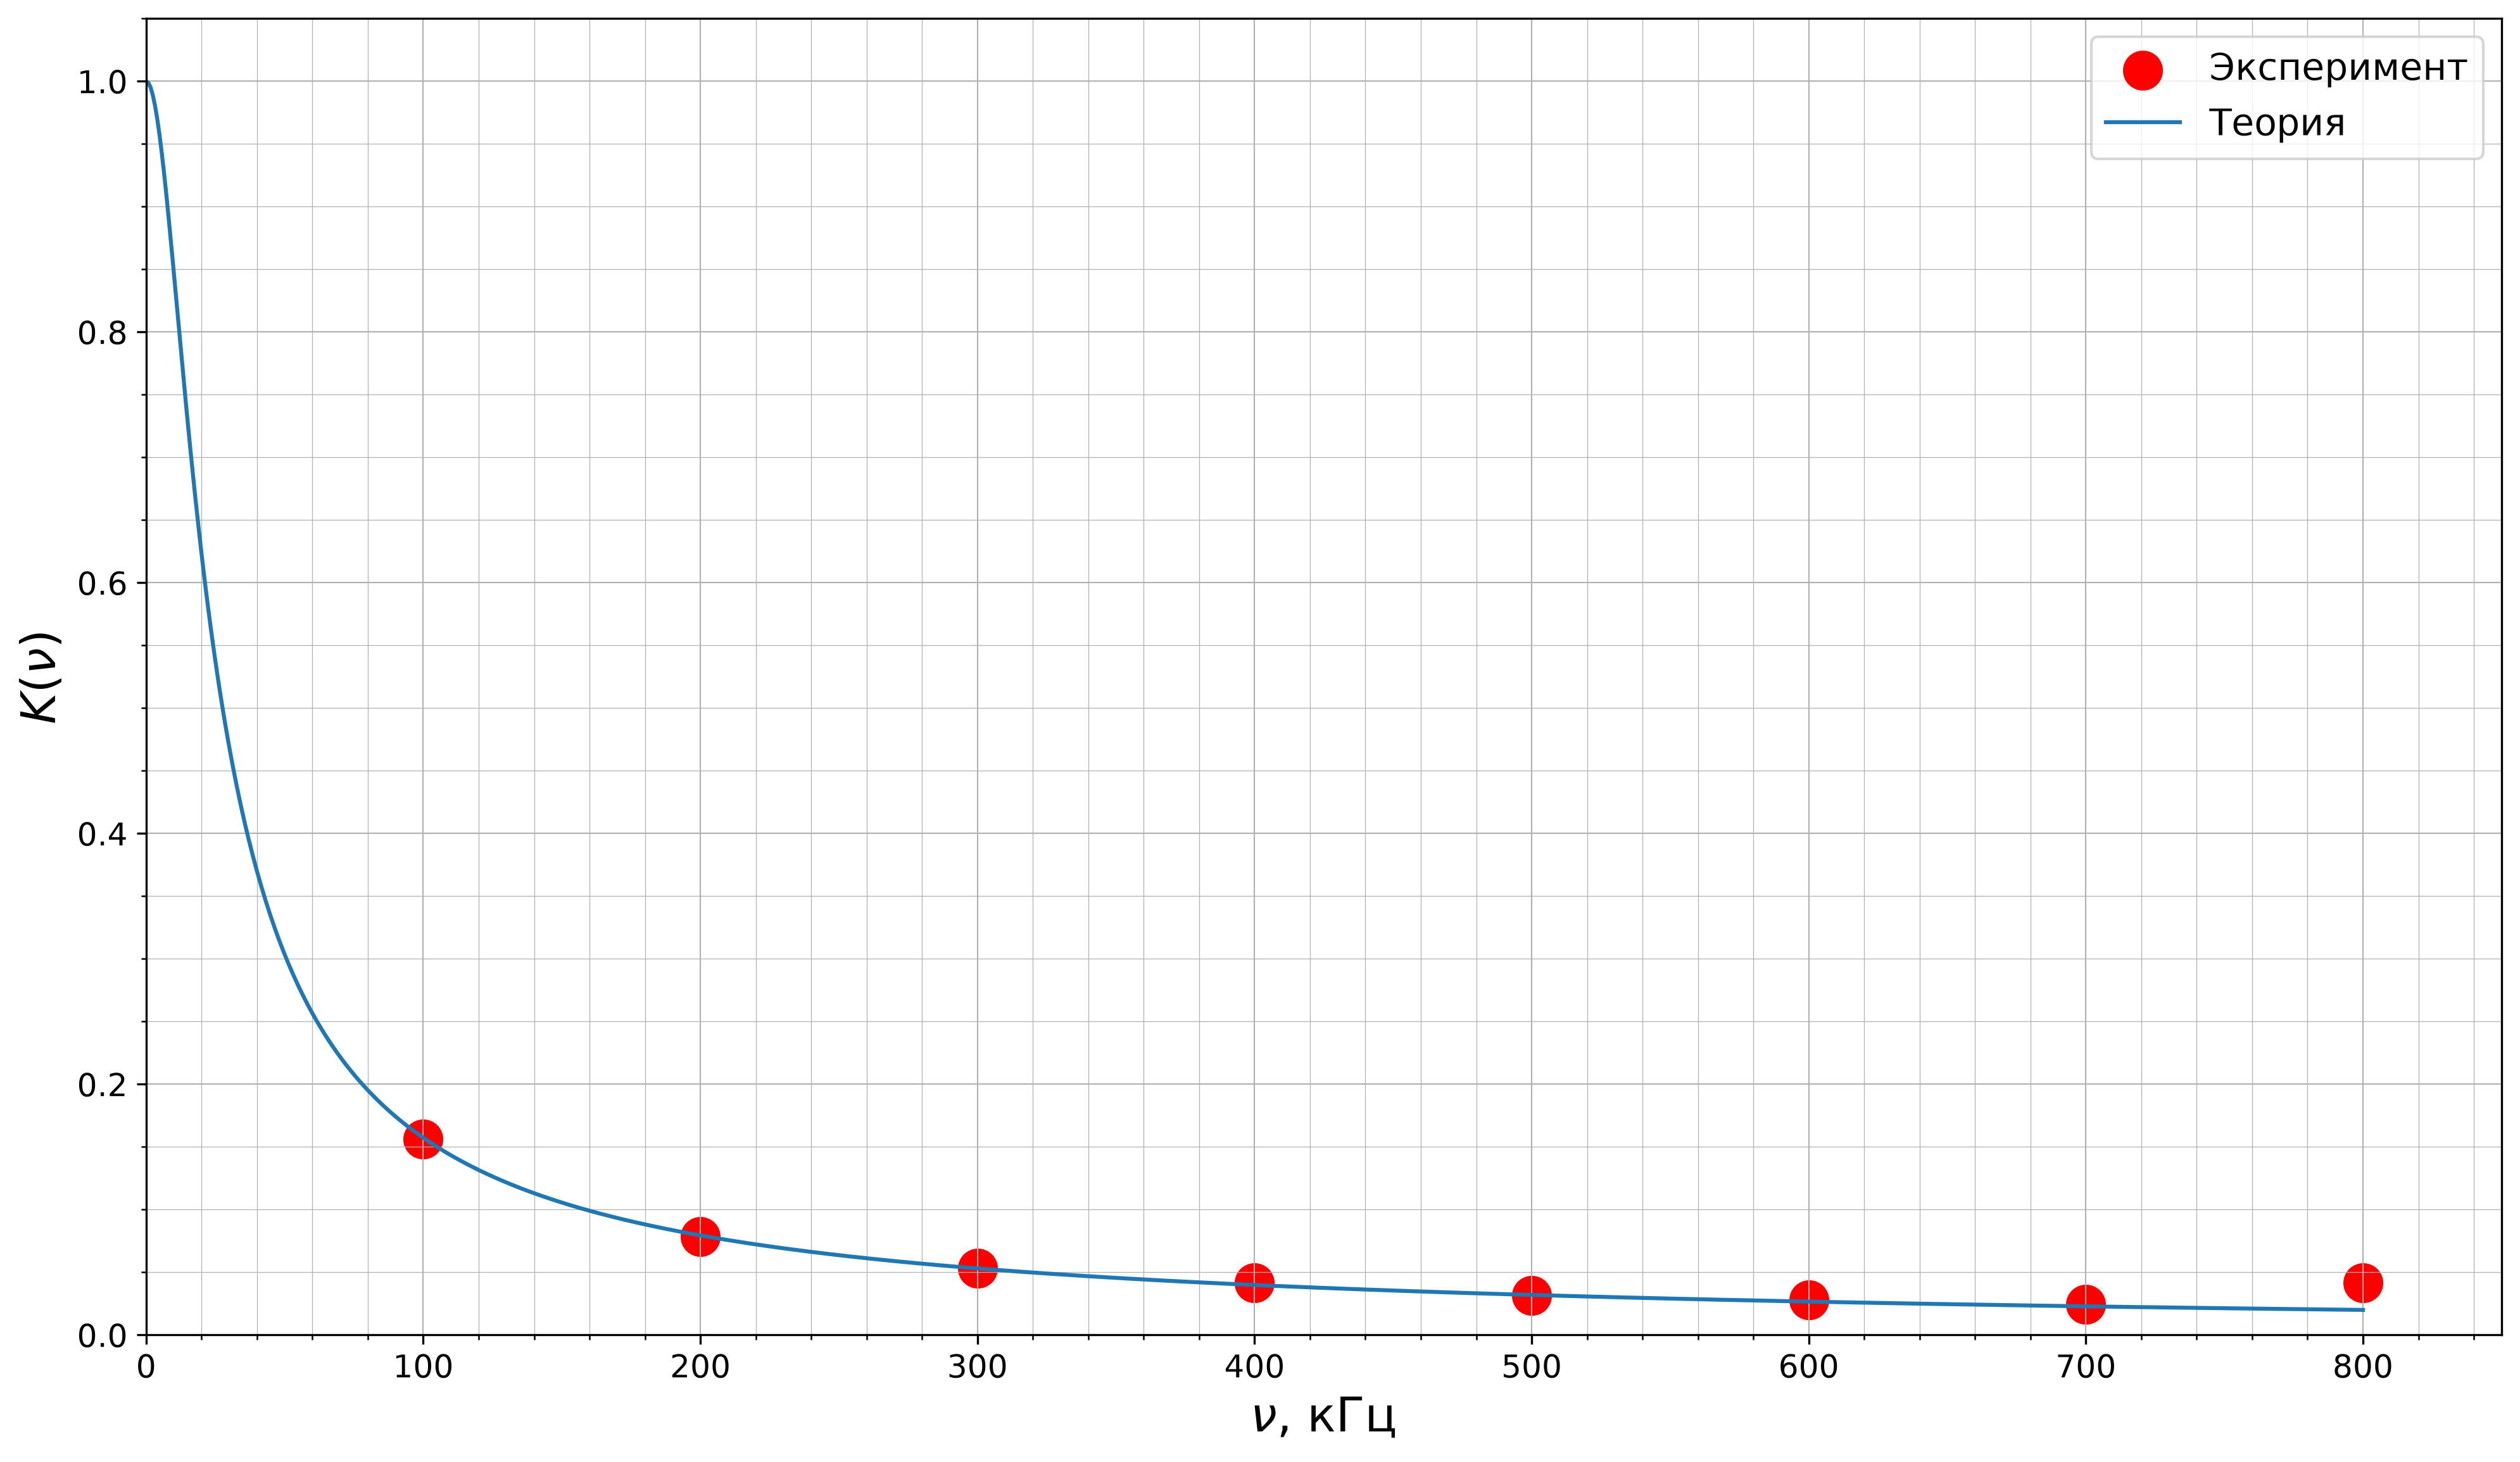
\includegraphics[width=1\textwidth]{images/K_nu.png}
    \caption{Зависимость коэффициента фильтрации $K$ от частоты $\nu$.}
    \label{fig:K_nu}
\end{figure}

Экспериментальные значения коэффициента фильтрации сравнивались
с теоретической зависимостью
\[
K(\nu)=\frac{1}{\sqrt{1+(2\pi\nu\tau_{RC})^2}}.
\]

По экспериментальным данным получено значение постоянной времени
RC-цепочки
\[
\boxed{\tau_{RC}\approx10~\text{мкс}}.
\]

Теоретическая зависимость, рассчитанная для
$\tau_{RC}=10~\text{мкс}$, хорошо согласуется с экспериментальными
данными. С увеличением частоты коэффициент фильтрации уменьшается,
что свидетельствует о подавлении высокочастотных гармоник
RC-фильтром.

\subsection{Определение постоянной времени}

По параметрам RC-цепочки расчётное значение постоянной времени
составляет
\[
\tau_{RC}^{\text{расч}}=RC=3~\text{мкс}.
\]

Для экспериментального определения постоянной времени использовалось
соотношение
\[
K(\nu)=\frac{1}{\sqrt{1+(2\pi\nu\tau_{RC})^2}},
\]
откуда
\[
\tau_{RC}=
\frac{\sqrt{1/K^2-1}}{2\pi\nu}.
\]

По первым семи экспериментальным точкам получено
\[
\boxed{\tau_{RC}^{\text{эксп}}=(9{.}86\pm0{.}12)~\text{мкс}}.
\]

Экспериментальное значение отличается от расчётного, что указывает
на наличие систематической погрешности определения коэффициента
фильтрации или параметров реальной RC-цепочки.

% TODO: погрешность


% =========================================================
% ОБЩИЙ ВЫВОД
% =========================================================

\section*{Вывод}

В работе исследованы спектры электрических сигналов. Для прямоугольных
импульсов при $\tau=20\text{--}200~\text{мкс}$ получено
$\Delta\nu=48{.}62\text{--}4{.}93~\text{кГц}$, при этом
$\Delta\nu\tau\approx0{.}96$. При $T=200\text{--}5000~\text{мкс}$
расстояние между соседними гармониками составило
$\delta\nu=4{.}98\text{--}0{.}20~\text{кГц}$, причём
$\delta\nu T\approx1$.

Для цугов синусоидального сигнала исследованы значения
$N=5\text{--}20$, $T=1\text{--}4~\text{мс}$ и
$\nu_0=50\text{--}200~\text{кГц}$. Теорема смещения подтверждена:
$\nu_{\text{ц}}=\nu_0$.

Для АМ-сигнала при $m=10\text{--}100\%$ отношение амплитуд
$a_{\text{бок}}/a_{\text{осн}}$ изменялось от $0{.}05$ до $0{.}51$;
коэффициент наклона экспериментальной зависимости составил
$0{.}516\pm0{.}009$ при теоретическом значении $0{.}5$.

Для RC-фильтра при $R=3~\text{кОм}$ и $C=1000~\text{пФ}$ расчётные
значения составили $\tau_{RC}=3~\text{мкс}$ и
$\nu_{RC}=333~\text{кГц}$. В диапазоне $\nu=100\text{--}800~\text{кГц}$
коэффициент фильтрации изменялся от $K=0{.}1560$ до $K=0{.}0241$.

\end{document}